\documentclass[11pt]{article}
\usepackage[T1]{fontenc}
\usepackage[utf8]{inputenc}
\usepackage{lmodern}
\ifdefined\pdfglyphtounicode
  \input{glyphtounicode}
  \pdfglyphtounicode{tfm:lmex10/parenleftbig}{0028}
  \pdfglyphtounicode{tfm:lmex10/parenrightbig}{0029}
  \pdfglyphtounicode{tfm:lmex10/bracketleftbig}{005B}
  \pdfglyphtounicode{tfm:lmex10/bracketrightbig}{005D}
  \pdfglyphtounicode{tfm:lmex10/parenleftBig}{0028}
  \pdfglyphtounicode{tfm:lmex10/parenrightBig}{0029}
  \pdfglyphtounicode{tfm:lmex10/parenleftbigg}{0028}
  \pdfglyphtounicode{tfm:lmex10/parenrightbigg}{0029}
  \pdfglyphtounicode{tfm:lmex10/bracketleftbigg}{005B}
  \pdfglyphtounicode{tfm:lmex10/bracketrightbigg}{005D}
  \pdfglyphtounicode{tfm:lmex10/parenleftBigg}{0028}
  \pdfglyphtounicode{tfm:lmex10/parenrightBigg}{0029}
  \pdfglyphtounicode{tfm:lmex10/bracketleftBigg}{005B}
  \pdfglyphtounicode{tfm:lmex10/bracketrightBigg}{005D}
  \pdfglyphtounicode{tfm:lmex10/braceleftBigg}{007B}
  \pdfglyphtounicode{tfm:lmex10/bracerightBigg}{007D}
  \pdfglyphtounicode{tfm:lmex10/bracketleftBig}{005B}
  \pdfglyphtounicode{tfm:lmex10/bracketrightBig}{005D}
  \pdfglyphtounicode{tfm:lmex10/braceleftBig}{007B}
  \pdfglyphtounicode{tfm:lmex10/bracerightBig}{007D}
  \pdfglyphtounicode{tfm:lmex10/vextendsingle}{23D0}
  \pdfglyphtounicode{tfm:lmex10/vextenddouble}{2016}
  \pdfglyphtounicode{tfm:lmex10/bracelefttp}{23A7}
  \pdfglyphtounicode{tfm:lmex10/braceleftbt}{23A9}
  \pdfglyphtounicode{tfm:lmex10/braceleftmid}{23A8}
  \pdfglyphtounicode{tfm:lmex10/braceex}{23AA}
  \pdfglyphtounicode{tfm:lmex10/summationtext}{2211}
  \pdfglyphtounicode{tfm:lmex10/summationdisplay}{2211}
  \pdfglyphtounicode{tfm:lmex10/hatwide}{02C6}
  \pdfglyphtounicode{tfm:lmex10/hatwider}{02C6}
  \pdfglyphtounicode{tfm:lmex10/tildewide}{02DC}
  \pdfglyphtounicode{tfm:lmex10/tildewider}{02DC}
  \pdfglyphtounicode{tfm:lmex10/radicalbig}{221A}
  \pdfglyphtounicode{tfm:lmex10/radicalBig}{221A}
  \pdfglyphtounicode{tfm:lmsy10/mapsto}{007C}
  \pdfglyphtounicode{tfm:lmsy10/A}{1D49C}
  \pdfglyphtounicode{tfm:lmsy10/C}{1D49E}
  \pdfglyphtounicode{tfm:lmsy10/D}{1D49F}
  \pdfglyphtounicode{tfm:lmsy10/E}{2130}
  \pdfglyphtounicode{tfm:lmsy10/F}{2131}
  \pdfglyphtounicode{tfm:lmsy10/H}{210B}
  \pdfglyphtounicode{tfm:lmsy10/K}{1D4A6}
  \pdfglyphtounicode{tfm:lmsy10/L}{2112}
  \pdfglyphtounicode{tfm:lmsy10/M}{2133}
  \pdfglyphtounicode{tfm:lmsy10/T}{1D4AF}
  \pdfglyphtounicode{tfm:lmsy10/U}{1D4B0}
  \pdfglyphtounicode{tfm:lmsy10/V}{1D4B1}
  \pdfglyphtounicode{tfm:lmsy10/W}{1D4B2}
  \pdfglyphtounicode{tfm:lmsy10/X}{1D4B3}
  \pdfglyphtounicode{tfm:lmsy10/Y}{1D4B4}
  \pdfglyphtounicode{tfm:lmsy10/Z}{1D4B5}
  \pdfglyphtounicode{tfm:lmsy8/X}{1D4B3}
  \pdfglyphtounicode{tfm:msbm10/R}{211D}
  \pdfglyphtounicode{tfm:msbm10/S}{1D54A}
  \pdfglyphtounicode{tfm:rm-lmbx10/one}{1D7CF}
  \pdfglyphtounicode{tfm:esint10/acute}{222B}
  \pdfglyphtounicode{tfm:esint10/circumflex}{222B}
  \pdfglyphtounicode{tfm:esint10/space}{2A0F}
  \pdfglyphtounicode{tfm:lmmi10/mu}{03BC}
  \pdfglyphtounicode{tfm:lmmi8/mu}{03BC}
  \pdfglyphtounicode{tfm:rm-lmr10/Delta}{0394}
  \pdfglyphtounicode{tfm:rm-lmr10/Omega}{03A9}
  \pdfglyphtounicode{tfm:rm-lmr8/Omega}{03A9}
  \pdfgentounicode=1
\fi

\usepackage[margin=1in]{geometry}
\usepackage{amsmath,amssymb,amsthm,mathtools,esint}
\usepackage{microtype,needspace}
\usepackage{graphicx,booktabs,array,enumitem}
\usepackage{tikz}
\usetikzlibrary{arrows.meta,calc,positioning}
\usepackage[numbers,sort&compress]{natbib}
\usepackage[colorlinks=true,linkcolor=blue!45!black,citecolor=blue!45!black,urlcolor=blue!45!black]{hyperref}
\usepackage[nameinlink,noabbrev]{cleveref}
\newcommand{\R}{\mathbb R}
\newcommand{\N}{\mathbb N}
\newcommand{\eps}{\varepsilon}
\newcommand{\dd}{\,\mathrm d}
\newcommand{\Id}{\mathrm{Id}}
\newcommand{\cH}{\mathcal H}
\DeclareMathOperator{\dist}{dist}
\DeclareMathOperator{\supp}{supp}
\DeclareMathOperator{\osc}{osc}
\DeclareMathOperator{\tr}{tr}
\DeclareMathOperator{\sech}{sech}
\newtheorem{theorem}{Theorem}[section]
\newtheorem{proposition}[theorem]{Proposition}
\newtheorem{lemma}[theorem]{Lemma}
\newtheorem{corollary}[theorem]{Corollary}
\theoremstyle{definition}
\newtheorem{definition}[theorem]{Definition}
\theoremstyle{remark}
\newtheorem{remark}[theorem]{Remark}
\numberwithin{equation}{section}
\setlist[enumerate]{itemsep=3pt}
\setlist[itemize]{itemsep=3pt}
\setlength{\emergencystretch}{2em}
\allowdisplaybreaks[2]
\hypersetup{pdftitle={A positive resolution of De Giorgi's conjecture in dimension eight},pdfauthor={OpenAI}}
\title{A positive resolution of De Giorgi's conjecture\\in dimension eight}
\author{OpenAI}
\date{September 26, 2026}
\begin{document}
\maketitle
\begin{abstract}
We resolve De Giorgi's conjecture positively in dimension eight:
every entire $C^2$ solution $u:\R^8\to(-1,1)$ of
$\Delta u=u^3-u$ with an everywhere positive directional derivative
is a planar heteroclinic. We prove that every stable solution
$v:\R^7\to[-1,1]$ of this equation is a constant well or a planar heteroclinic,
without an energy-growth assumption.
\end{abstract}
\section{Introduction}\label{sec:introduction}

Consider the scalar Allen--Cahn equation
\begin{equation}\label{eq:allen-cahn}
 \Delta u=u^3-u.
\end{equation}
The function
\[
 g(s)=\tanh(s/\sqrt2)
\]
is its increasing one-dimensional transition from $-1$ to $1$.
Thus $u(x)=g(e\cdot x-c)$ solves \eqref{eq:allen-cahn} whenever
$e$ is a unit vector; its level sets are parallel hyperplanes.
De Giorgi's conjecture asks whether every bounded entire solution
that is strictly increasing in a fixed direction has this form in
ambient dimension at most eight \cite{DeGiorgi1979}.

The conjecture connects phase transitions with the Bernstein problem
for minimal hypersurfaces.  For the quartic potential
\[
 W(s)=\frac14(1-s^2)^2,
\]
the rescaled phase-transition energies have surface tension times
perimeter as their variational limit
\cite{ModicaMortola1977,Modica1987}.
The graph condition in the minimal-surface problem is important:
nonflat minimizing cones occur in ambient dimension eight, whereas
nonaffine entire minimal graphs first occur in ambient dimension nine
\cite{Simons1968,BDG1969}.
The corresponding distinction between stable and monotone
Allen--Cahn solutions will also enter our proof.

Theorem~\ref{thm:stable} has a geometric parallel in the stable Bernstein
theorem for complete, connected, two-sided stable smooth minimal immersions
of boundaryless six-manifolds into $\R^7$: their images are entire affine
hyperplanes, with no volume-growth hypothesis
\cite[Theorem~1.1]{HongLiWang2026}.
The Bernstein theorem is not an input to our argument.

Ghoussoub and Gui established the conjecture in dimension two
\cite{GhoussoubGui1998}, and Ambrosio and Cabr\'e in dimension three
\cite{AmbrosioCabre2000}.
Savin proved the result through dimension eight under the additional
assumption
\[
 \lim_{t\to-\infty}u(x',t)=-1,\qquad
 \lim_{t\to+\infty}u(x',t)=1
 \quad\text{for every }x'\in\R^{n-1}
\]
\cite[Theorem~2.4]{Savin2009}.
These limits are pointwise in the transverse variable.
Del Pino, Kowalczyk and Wei constructed nonplanar strictly monotone
solutions in every ambient dimension at least nine, near large
dilations of nonaffine minimal graphs \cite{DPKW2011}.
The main result of this paper gives a positive resolution in
dimension eight without an assumption on the directional
limits.

\begin{theorem}[Monotone rigidity in dimension eight]
\label{thm:monotone}
Let $u\in C^2(\R^8,(-1,1))$ satisfy
\[
 \Delta u=u^3-u,\qquad \partial_8u>0\quad\text{in }\R^8.
\]
Then there are $e\in\mathbb S^7$ with $e_8>0$ and $c\in\R$ such that
\[
 u(x)=\tanh\!\left(\frac{e\cdot x-c}{\sqrt2}\right)
 \qquad\text{for every }x\in\R^8.
\]
\end{theorem}

Neither energy growth nor minimization is assumed.  Those properties,
and the well limits, will be consequences of the argument.
Both rigidity theorems concern the scalar quartic equation
\eqref{eq:allen-cahn}; the monotonicity assumption in
Theorem~\ref{thm:monotone} is strict positivity of $\partial_8u$.

\subsection{The stable equation}

For an open set $\Omega\subset\R^n$ write
\[
 \mathcal E(v;\Omega)
   =\int_\Omega\left(\frac12|\nabla v|^2+W(v)\right)\dd x.
\]
A solution $v$ is \emph{stable} if its second variation satisfies
\begin{equation}\label{eq:stability-definition}
 Q_v(\varphi):=
 \int_{\R^n}\bigl(|\nabla\varphi|^2+(3v^2-1)\varphi^2\bigr)\dd x
 \ge0
 \qquad\text{for every }\varphi\in C_c^1(\R^n).
\end{equation}
A \emph{global minimizer} minimizes $\mathcal E$ in every ball
among $H^1$ competitors with the same boundary trace.
Stability requires only the quadratic inequality, so it is a weaker
condition than minimization.

A strictly positive directional derivative solves the linearized
equation and gives stability.  Moreover, the limits along that
direction are stable solutions in one fewer variable.
This observation makes the following classification the analytic
core of the paper.

\begin{theorem}[Stable rigidity in dimension seven]
\label{thm:stable}
Let $v\in C^2(\R^7,[-1,1])$ be a stable solution of
$\Delta v=v^3-v$.  Then either $v\equiv1$, $v\equiv-1$, or
\[
 v(x)=\tanh\!\left(\frac{a\cdot x-b}{\sqrt2}\right)
 \qquad\text{for some }a\in\mathbb S^6,\ b\in\R.
\]
No energy-growth assumption is required.
\end{theorem}

This stability endpoint is sharp: Pacard and Wei constructed bounded
stable nonplanar solutions in dimension eight
\cite{PacardWei2013}.
For the smooth quartic equation, Liu, Luo, Wang, Juncheng Wei,
Yong Wei and Wu prove stable rigidity in dimension three and
monotone rigidity in dimension four \mbox{\cite{LLWWW2026}.}
The same conclusions are obtained independently by Chan, Fern\'andez-Real,
Figalli, Florit-Simon and Serra
\cite[Theorem~1.1 and Corollary~1.2]{CFFFS2026}.
Florit-Simon and Serra prove stable rigidity in dimension four
under a bounded-energy-density hypothesis \cite{FSS2025}.
Both the higher dimension and the removal of the density assumption
matter here; they require different parts of the analysis.

\subsection{From stable end profiles to the monotone theorem}

We give the complete deduction of Theorem~\ref{thm:monotone} from
Theorem~\ref{thm:stable} at the beginning of the paper.
The comparison with competitors between the directional limits is due
to Alberti, Ambrosio and Cabr\'e
\cite[Theorem~4.4]{AlbertiAmbrosioCabre2001}.
Jerison and Monneau established the minimizing-end-profile reduction
\cite[Theorem~1.3]{JerisonMonneau2004}.
The positive derivative supplies stability, and the directional
limits are stable seven-dimensional solutions.  Their classification
allows constant wells or planar transitions at this stage.
Each is a global minimizer, by the one-dimensional calibration.
Clipping a competitor between the two end profiles and sliding
translates of $u$ then shows that $u$ is itself a global minimizer.
Comparison with a constant phase inside a large ball gives
$\mathcal E(u;B_R)\le CR^7$.

The surface tension in this normalization is
\begin{equation}\label{eq:intro-tension}
 s_0=\int_{-1}^1\sqrt{2W(t)}\dd t
     =\int_\R g'(s)^2\dd s
     =\frac{2\sqrt2}{3}.
\end{equation}
Under dilations $u(R_jx)$ with $R_j\to\infty$, the minimizing
comparison identifies the entire limiting energy measure with
$s_0$ times the perimeter measure of a minimizing boundary.
This equality needs a recovery sequence patched to the original
solution; convergence of the phases alone would leave open the
possibility of extra energy.

Energy monotonicity makes the limiting boundary a cone, that is,
a boundary preserved by dilations about the origin.
Directional monotonicity fixes the sign of one component of its
normal.  In dimension eight the minimizing-boundary regularity
theory allows only a possible singularity at the vertex
\cite{Federer1970}.
The classical directed-cone argument then forces a hyperplane
\cite{Schnuerer2003}.  We include the case in which that normal
component vanishes identically: it gives translation invariance,
which is incompatible with an isolated singular vertex.
The limiting density is therefore that of one planar transition.
Wang's near-unit-density theorem
\cite[Theorem~11.1]{Wang2017} returns to the original solution,
and the one-dimensional equation determines the profile and its
orientation.

This deduction explains why the stable theorem is the right target.
It also separates the classical geometric reduction from the new
estimates needed for stable solutions.  A reader interested primarily
in the conjecture can follow the deduction first; a reader interested
in the stable classification can proceed directly from its statement
to the analytic argument in Part II.
The classical gradient bound and energy monotonicity needed by both
paths are proved in Section~\ref{sec:classical-estimates}.

\subsection{The finite-density step}

Let $\omega_{n-1}$ be the volume of the unit ball in $\R^{n-1}$.
For a solution in $\R^n$ define
\[
 M_R(y)=\frac{\mathcal E(v;B_R(y))}
              {s_0\omega_{n-1}R^{n-1}},\qquad
 M_\infty=\sup_{R>0}M_R(0).
\]
A single planar transition has limiting density one.
The first analytic step is the following result, which is also
needed locally in the argument that removes the density bound.

\begin{theorem}[Finite-density stable rigidity]\label{thm:finite}
Let $4\le n\le7$.  Suppose $v\in C^2(\R^n,[-1,1])$ solves
$\Delta v=v^3-v$ and satisfies
\[
 \int_{\R^n}\bigl(|\nabla\varphi|^2+(3v^2-1)\varphi^2\bigr)\dd x
 \ge0
 \qquad\text{for every }\varphi\in C_c^1(\R^n).
\]
If $M_\infty<\infty$, then $v\equiv1$, $v\equiv-1$, or
$v(x)=g(a\cdot x-b)$ for some $a\in\mathbb S^{n-1}$ and $b\in\R$.
\end{theorem}

For stable solutions in $\R^7$, the remaining task is to prove that
$M_\infty$ is finite. A penalized reach measures both the bending of a
zero sheet and its proximity to other sheets; the finite-density theorem
supplies local regularity at nearly this scale. Combining reach geometry
with stability bounds the fourth curvature moment and squared defect,
controlling the regions where the zero set is poorly approximated by
planes. We then compare the reach inequality with an ambient stability
test built from the same radial amplitude on the sheets. The cost of
joining neighboring amplitudes is small enough to leave a strict positive
margin, which contradicts the amount of surface area forced by unbounded
density.

\subsection{Organization and conventions}

Part I gives the complete deduction from stable end profiles to
Theorem~\ref{thm:monotone}, conditional on
Theorem~\ref{thm:stable}.
Appendix~\ref{sec:dimension-nine} explains compatibility with the
dimension-nine construction of del Pino, Kowalczyk and Wei.
After an optional guide to the analytical strategy in
Section~\ref{sec:analytic-strategy}, Part II proves the diffuse estimates,
Theorem~\ref{thm:finite}, and its local regularity consequence.
Part III develops the reach and interface estimates, joins the
ambient and surface tests, and proves fourth-moment growth.
Part IV constructs the radial ambient test and completes the
unbounded-density contradiction.
Thus the reading order places the geometric application first,
while the analytic proof of the stable theorem is contained in
Parts II--IV.  For a direct analytical reading, begin at
Section~\ref{sec:diffuse}, whose opening recalls the equation, stability
and all normalizations used there; the strategy section can be read
beforehand or consulted later.

We write $n=m+1$, so $m$ is the interface dimension, and use
$\dd S$ for induced surface measure.
The surface tension $s_0$ and the normal-average constant
$\sigma=2s_0$ are kept distinct.
All stability tests are unrestricted compactly supported tests.
Uniformity in translating centers, the order of parameter choices,
and successive limits are specified in the statements where
they are needed.

\setcounter{tocdepth}{1}
\begingroup
\small
\tableofcontents
\endgroup
\section{Two classical estimates for the quartic equation}
\label{sec:classical-estimates}

Both the geometric deduction and the analytical classification use the
same gradient bound and energy monotonicity. We record their short
proofs here, independently of either rigidity theorem. Let $n=m+1\ge2$
and let $v\in C^2(\R^n,[-1,1])$ solve $\Delta v=v^3-v$.
Throughout,
\[
 W(t)=\frac14(1-t^2)^2,\qquad s_0=\frac{2\sqrt2}{3},
\]
and $\omega_m$ denotes the volume of the unit ball in $\R^m$.
Interior elliptic estimates bootstrap $v$ to a smooth function with
uniform bounds for every derivative of fixed order.

\subsection{Modica's gradient estimate}

We use Modica's gradient bound \cite{Modica1985},
\begin{equation}\label{eq:diffuse-modica}
 \frac12|\nabla v|^2\le W(v).
\end{equation}
For completeness, its entire-solution argument in this normalization is
short. For $P=|\nabla v|^2/2-W(v)$, the identities
$\nabla P=\nabla^2v\nabla v-W'(v)\nabla v$ and
$\Delta P=|\nabla^2v|^2-W'(v)^2$ imply, wherever $\nabla v\ne0$,
\[
 \Delta P\ge
 \frac{2W'(v)}{|\nabla v|^2}\nabla v\cdot\nabla P.
\]
If $\sup P>0$, translate a maximizing sequence and pass to a locally smooth
limit. Its $P$ attains a positive maximum. The strong maximum principle
makes $P$ constant on the component of $\{\nabla v\ne0\}$ containing that
point. This component is also closed: on it
$|\nabla v|^2\ge2\sup P>0$. It is therefore all of $\R^n$. The globally
bounded smooth vector field $\nabla v$ has complete forward flow, and along
that flow $v$ increases at rate at least $2\sup P$, contradicting its
boundedness. This proves \eqref{eq:diffuse-modica}.

\subsection{Normalized energy and monotonicity}

We recall Modica's energy monotonicity formula \cite{Modica1989} and
give the stress-tensor calculation in the present normalization. Set
\begin{equation}\label{eq:finite-density}
 e(v)=\frac12|\nabla v|^2+W(v),\qquad
 M_r(y)=\frac{1}{s_0\omega_m r^m}\int_{B_r(y)}e(v),\qquad
 M_\infty=\sup_{r>0}M_r(0).
\end{equation}
The stress tensor
\(e(v)\Id-\nabla v\otimes\nabla v\) is divergence free.  Its contraction with
the derivative of \(x-y\), followed by the divergence theorem, gives
\[
 r\int_{\partial B_r(y)}\bigl(e(v)-|\partial_rv|^2\bigr)
   =\int_{B_r(y)}\bigl((m+1)e(v)-|\nabla v|^2\bigr).
\]
Consequently
\begin{equation}\label{eq:finite-monotonicity}
 M_r'(y)=\frac{1}{s_0\omega_m}
 \left\{r^{-m-1}\int_{B_r(y)}\left(W(v)-\frac12|\nabla v|^2\right)
       +r^{-m}\int_{\partial B_r(y)}|\partial_rv|^2\right\}\ge0.
\end{equation}
The formula initially holds for almost every \(r\) and hence in integrated
form for every pair of radii.  Containment of shifted balls shows that the
limit at infinity is independent of \(y\), and \(M_r(y)\le M_\infty\).

The derivation uses neither stability nor a density-growth hypothesis.


\Needspace{12\baselineskip}
\part{The geometric deduction}
\section{From stable end profiles to the monotone theorem}
\label{sec:monotone}

In this part we deduce Theorem~\ref{thm:monotone} from the unrestricted
seven-dimensional classification in Theorem~\ref{thm:stable}, whose
independent analytical proof occupies Parts II--IV.  None of those parts
uses the geometric deduction given here.  The end
profiles will initially be allowed to be planar heteroclinics.  Their
minimizing property suffices for the argument; no well limit is imposed on
the given solution.  We first derive minimization and surface-order energy
growth, then identify the complete limiting energy with perimeter.  Only
after this exact identification do we use the geometry of a directed
minimizing cone and return to the equation at unit density.

We use the energy $\mathcal E$ and global minimizers defined in
Section~\ref{sec:introduction}.  It is enough to consider
competitors valued in $[-1,1]$: truncation to this interval decreases both
terms of the energy.  This definition also gives minimization in every
bounded Lipschitz domain: extend a same-trace competitor by $u$ to a
containing ball, use the Sobolev gluing property across the boundary, and
cancel the identical exterior energies.  We retain the normalization
\begin{equation}
 s_0=\int_{-1}^1\sqrt{2W(a)}\dd a
     =\int_\R g'(s)^2\dd s
     =\frac{2\sqrt2}{3}=\frac\sigma2.
 \label{eq:monotone-tension}
\end{equation}

\subsection{Stable end profiles and a variational comparison}

The first task is to turn strict monotonicity into minimizing barriers.
The positive directional derivative gives stability, and a long-cylinder
test transfers that stability to the seven-dimensional limits.  Their
classification then supplies a calibration, even when a limit is a planar
profile rather than a constant well.

\begin{lemma}[End profiles]
\label{lem:monotone-ends}
Let $u\in C^2(\R^8,(-1,1))$ solve $\Delta u=u^3-u$ and satisfy
$u_8>0$.  There are smooth stable solutions
$v_-,v_+:\R^7\to[-1,1]$ such that
\begin{equation}
 u(x',t+s)\longrightarrow v_\pm(x')
 \quad\text{in }C^k_{\mathrm{loc}}(\R^8)
 \quad\text{as }s\to\pm\infty,
 \qquad k\ge0.
 \label{eq:monotone-end-convergence}
\end{equation}
They satisfy $v_-(x')<u(x',t)<v_+(x')$ everywhere.  Their extensions
independent of the eighth coordinate are global minimizers in $\R^8$.
\end{lemma}

\begin{proof}
Elliptic interior estimates, applied on unit balls, give smoothness and
uniform bounds for every fixed derivative order of $u$.  The function
$h=u_8>0$ satisfies $(-\Delta+3u^2-1)h=0$.  For every compactly supported
$C^1$ function $\eta$, integration by parts gives the ground-state identity
\begin{equation}
 \int_{\R^8}\bigl(|\nabla\eta|^2+(3u^2-1)\eta^2\bigr)
   =\int_{\R^8}h^2\left|\nabla\left(\frac\eta h\right)\right|^2
   \ge0.
 \label{eq:monotone-ground-state}
\end{equation}
The division is legitimate because $h$ has a positive minimum on the
support of $\eta$.

Bounded monotonicity gives pointwise limits along each vertical line.
Translation compactness and the derivative bounds improve this to
\eqref{eq:monotone-end-convergence}.  Indeed every convergent subsequence
has the same pointwise limit, and a bounded vertical shift leaves that
limit unchanged.  Passing the equation and stability to these limits first
gives solutions and stability in eight dimensions.  To see stability in
seven dimensions, fix $\varphi\in C_c^1(\R^7)$ and a nonzero
$\zeta\in C_c^1(\R)$.  Test with
$\eta(x',t)=\varphi(x')\zeta(t/L)$ and divide by
$L\int\zeta^2$.  The result is
\[
 \int_{\R^7}\bigl(|\nabla\varphi|^2+(3v_\pm^2-1)\varphi^2\bigr)
 \ge -\frac1{L^2}\frac{\int|\zeta'|^2}{\int\zeta^2}
                         \int_{\R^7}\varphi^2.
\]
Letting $L\to\infty$ proves the assertion.  For example,
$u(x',t)<u(x',t+1)\le v_+(x')$, which proves the strict upper
inequality; the lower one is analogous.

Theorem~\ref{thm:stable} says that each $v_\pm$ is a constant well or
a planar heteroclinic.  To check the minimizing assertion directly, put
$\Phi(a)=\int_{-1}^a\sqrt{2W(b)}\dd b$.  For a unit vector $e$ and a
competitor $w\in H^1(\Omega,[-1,1])$,
\begin{equation}
 \frac12|\nabla w|^2+W(w)
    \ge \sqrt{2W(w)}\,\partial_e w
    =\partial_e\Phi(w).
 \label{eq:monotone-calibration}
\end{equation}
There is equality when $w(x)=g(e\cdot x-c)$, since
$g'=\sqrt{2W(g)}$.  The integral of the last expression depends only
on the boundary trace.  Thus such a profile minimizes on every ball, in
any ambient dimension in which $e$ is a unit vector.  This includes the
extensions of the seven-dimensional profiles, with $e_8=0$.  The
constants $\pm1$ have zero energy and also minimize.
\end{proof}

The next comparison also applies in other dimensions.  It records exactly
which property of the end profiles is used.  The constrained comparison
between end profiles was proved by Alberti, Ambrosio and Cabr\'e
\cite[Theorem~4.4]{AlbertiAmbrosioCabre2001}.  The unrestricted
minimization implication is the classical theorem of
\citet[Theorem~1.3, p.~441; proof on pp.~452--453]{JerisonMonneau2004};
we include the compact comparison argument in the present normalization.
Its globally $C^{1,1}$ potential hypothesis is met by
\[
 \widetilde W(s)=
 \begin{cases}
  (s+1)^2,&s<-1,\\
  W(s),&-1\le s\le1,\\
  (s-1)^2,&s>1.
 \end{cases}
\]
The values and the first two derivatives match at the wells, and
$\widetilde W'$ is globally Lipschitz.  Both potentials are nonnegative
and agree on $[-1,1]$.  Clipping any competitor to this interval decreases
its gradient energy and replaces its exterior potential by zero for
either potential, so their minimizing comparisons for $u$ agree.

\begin{lemma}[Minimizing barriers and compact sliding]
\label{lem:monotone-minimizer}
Let $N\ge2$, and suppose a bounded solution
$u:\R^{N-1}\times\R\to(-1,1)$ of $\Delta u=W'(u)$ is strictly
increasing in the last coordinate.  Suppose its vertical limits
$a_\pm(x')$, extended to $\R^N$, are global minimizers.  Then $u$ is a
global minimizer.  Moreover there is a dimensional constant $C_N$ such
that
\begin{equation}
 \mathcal E(u;B_R(y))\le C_N R^{N-1}
 \qquad (y\in\R^N,\ R\ge2).
 \label{eq:monotone-energy-growth}
\end{equation}
\end{lemma}

\begin{proof}
Fix a ball $B$.  The direct method produces an energy minimizer $w$ with
boundary trace $u$; truncation allows $|w|\le1$.  First clip it from
below by $a_-$, writing $w_1=\max\{w,a_-\}$.  The Sobolev lattice
identity is
\[
 \mathcal E(\max\{w,a_-\};B)
 +\mathcal E(\min\{w,a_-\};B)
 =\mathcal E(w;B)+\mathcal E(a_-;B).
\]
Since $u>a_-$ on $\partial B$, the minimum on the left has the same
trace as $a_-$.  Minimality of $a_-$ therefore shows
$\mathcal E(w_1;B)\le\mathcal E(w;B)$.  The maximum has trace $u$,
so it remains an unconstrained minimizer.  The analogous upper clipping
gives another unconstrained minimizer
$\widetilde w=\min\{w_1,a_+\}$ satisfying
$a_-\le\widetilde w\le a_+$.

The Euler--Lagrange equation and elliptic boundary regularity make
$\widetilde w$ smooth up to $\partial B$.  A difference of two
solutions $b,c$ here satisfies
$-\Delta(b-c)+(b^2+bc+c^2-1)(b-c)=0$, with bounded zeroth-order
coefficient.  Strong comparison for a nonnegative solution of this
linear equation, together with the strict boundary inequalities, gives
\[
 a_-<\widetilde w<a_+\quad\text{on }\overline B.
\]
These gaps have positive minima on this compact set.  Vertical translates
$u_s(x',t)=u(x',t+s)$ converge uniformly there to $a_+$ as
$s\to+\infty$, so $u_s>\widetilde w$ for all sufficiently large $s$.
Let
\[
 s_* =\inf\{s\ge0:u_s\ge\widetilde w\text{ on }\overline B\}.
\]
The set inside the infimum is an upper interval, by strict monotonicity.
Continuity gives $u_{s_*}\ge\widetilde w$.  If $s_*>0$, then
$u_{s_*}>u=\widetilde w$ on $\partial B$, and strong comparison gives
strict inequality throughout $\overline B$.  Compactness and continuity
then allow a smaller positive translation, a contradiction.  Thus
$\widetilde w\le u$.  For the reverse inequality, $u_{-s}$ lies below
$\widetilde w$ when $s$ is large.  Decrease $s\ge0$ until first
contact.  A positive first-contact parameter is again impossible, because
$u_{-s}<u=\widetilde w$ on $\partial B$ and strong comparison gives
a strict compact gap.  At $s=0$ this yields $u\le\widetilde w$.
Consequently $u=\widetilde w$ on $B$, and $B$ was arbitrary.

Finally choose a smooth cutoff $\eta_R$ that is zero on $B_{R-1}(y)$,
one near $\partial B_R(y)$, and satisfies $|\nabla\eta_R|\le C$.
The competitor $1+\eta_R(u-1)$ has zero energy in the inner ball and
bounded energy density in the remaining shell.  The latter assertion
uses $|u|\le1$ and the uniform unit-scale interior gradient estimate for
the equation.  The shell has volume at most $C_NR^{N-1}$, proving
\eqref{eq:monotone-energy-growth}.
\end{proof}

Lemmas~\ref{lem:monotone-ends} and~\ref{lem:monotone-minimizer} apply to
the solution of Theorem~\ref{thm:monotone}.  They establish minimization
and the required energy growth directly from its hypotheses and
Theorem~\ref{thm:stable}.

\subsection{Exact convergence to a minimizing boundary}

We have obtained the variational comparison needed for the blow-down.
The remaining issue in this step is equality of measures: phase
convergence and a perimeter lower bound alone would permit additional
diffuse energy.  We eliminate that possibility by comparing with a
recovery sequence patched to the original solution in a thin annular
layer.  This argument does not require a prescribed trace for the
recovery sequence.

We use the following established variational and geometric inputs.
For a finite-perimeter set $F$ in a bounded Lipschitz domain $\Omega$,
the Modica--Mortola recovery theorem provides, for any sequence
$\eps_j\downarrow0$, functions
$w_j\in H^1(\Omega,[-1,1])$ such that
\begin{equation}
 \begin{split}
 w_j&\longrightarrow 2\mathbf1_F-1\quad\text{in }L^1(\Omega),\\
 \limsup_j\int_\Omega
   \left(\frac{\eps_j}2|\nabla w_j|^2+\frac{W(w_j)}{\eps_j}\right)
   &\le s_0 P(F;\Omega).
 \end{split}
 \label{eq:monotone-recovery}
\end{equation}
Here $P(F;\Omega)=|D\mathbf1_F|(\Omega)$ is relative perimeter
\citep{ModicaMortola1977}; the finite-perimeter recovery statement is
also proved in \citet[Section~3, pp.~140--141]{Modica1987}.
For a locally perimeter-minimizing set in
$\R^N$, its perimeter measure defines a stationary integral varifold
with multiplicity one on the reduced boundary.  Its support is a smooth
embedded minimal hypersurface outside a closed singular set of Hausdorff
dimension at most $N-8$ (and the singular set is empty when $N\le7$).
The centered area ratio is nondecreasing, and equality at all scales
forces a cone.  These are the classical regularity, dimension-reduction,
and monotonicity results for minimizing boundaries
\citep{Federer1969,Giusti1984,Simons1968}; for the sharp singular-set
dimension bound, see \citet[Theorem~1, p.~769]{Federer1970}.
The argument below uses
recovery and comparison to prove exact energy convergence before using
this multiplicity-one geometric theory.

\begin{proposition}[Exact perimeter limit]
\label{prop:monotone-exact-limit}
Let $u:\R^N\to[-1,1]$ be an entire global minimizer with
$\mathcal E(u;B_R)\le CR^{N-1}$ for $R\ge2$.  Given
$R_j\to\infty$, set $\eps_j=R_j^{-1}$ and $u_j(x)=u(R_jx)$.
After taking a subsequence there is a locally finite-perimeter set $E$
such that
\begin{equation}
 \begin{aligned}
 u_j&\longrightarrow 2\mathbf1_E-1
                    &&\text{in }L^1_{\mathrm{loc}}(\R^N),\\
 \left(\frac{\eps_j}2|\nabla u_j|^2+
                \frac{W(u_j)}{\eps_j}\right)\dd x
   &\rightharpoonup s_0|D\mathbf1_E|
                    &&\text{as local Radon measures}.
 \end{aligned}
 \label{eq:monotone-exact-limit}
\end{equation}
The set $E$ is locally perimeter minimizing against compact perturbations.
\end{proposition}

\begin{proof}
\emph{Compactness and the lower bound.}
Recall the phase primitive
$\Phi(a)=\int_{-1}^a\sqrt{2W(b)}\,\dd b$.
Denote the rescaled energy by $\mathcal E_j$ and its energy measure by
$\mu_j$.  Scaling the minimizing comparison shows that $u_j$ minimizes
$\mathcal E_j$ against every compact modification.  A change of variables
gives
\begin{equation}
 \mu_j(B_r)=R_j^{1-N}\mathcal E(u;B_{R_jr}).
 \label{eq:monotone-rescaled-energy}
\end{equation}
Thus these measures are locally bounded.  Moreover
\[
 |\nabla\Phi(u_j)|
   \le \frac{\eps_j}2|\nabla u_j|^2+\frac{W(u_j)}{\eps_j},
 \qquad \int_K W(u_j)\le\eps_j\mu_j(K)\longrightarrow0
\]
on each compact set $K$.  Local BV compactness, followed by a diagonal
subsequence, implies that $\Phi(u_j)$ has an $L^1_{\mathrm{loc}}$
limit.  The vanishing potential forces its values to lie in
$\{\Phi(-1),\Phi(1)\}=\{0,s_0\}$.  The inverse of $\Phi$ is
uniformly continuous on $[0,s_0]$, so this also proves the asserted
local $L^1$ convergence of $u_j$ to $2\mathbf1_E-1$.  Weak compactness
of $\mu_j$ and lower semicontinuity
of total variation give a local measure limit $\mu$ satisfying
\begin{equation}
 \mu\ge s_0|D\mathbf1_E|.
 \label{eq:monotone-perimeter-lower}
\end{equation}

\emph{A recovery comparison with the correct boundary trace.}
We prove the opposite inequality, including the boundary gluing.  Fix a
ball $B_r(y)$ and $\delta>0$.  Let $F$ be a finite-perimeter set in
$B_{r+\delta}(y)$ that agrees with $E$ on the annulus
$A=B_{r+\delta}(y)\setminus\overline{B_r(y)}$.  The case $F=E$
is permitted.  Choose a recovery sequence $w_j$ on this larger ball as
in \eqref{eq:monotone-recovery}.  Both $w_j$ and $u_j$ converge on $A$
to $2\mathbf1_E-1$.  Their boundedness implies
\begin{equation}
 \int_A|u_j-w_j|^2\le2\int_A|u_j-w_j|\longrightarrow0.
 \label{eq:monotone-annulus-mismatch}
\end{equation}

For $\eps_j<\delta/4$, partition all but a remainder of $A$ into
$L_j=\lfloor\delta/\eps_j\rfloor-1$ disjoint radial layers of
thickness $\eps_j$.  Thus $L_j\ge\delta/(2\eps_j)$, and the
outer remainder leaves a neighborhood of $\partial B_{r+\delta}(y)$
untouched.  In one such layer $S$, let $\chi$ increase from
zero to one, with $|\nabla\chi|\le C/\eps_j$, and interpolate by
$z_j=(1-\chi)w_j+\chi u_j$.  The cutoff is zero on the inner side
and one on the outer side.  On $[-1,1]$, boundedness of $W''$ and
$|W'|^2\le CW$ give, uniformly for $0\le\chi\le1$,
\[
 W((1-\chi)a+\chi b)
       \le C\bigl(W(a)+W(b)+|a-b|^2\bigr).
\]
Expanding the gradient therefore yields
\begin{equation}
 \mathcal E_j(z_j;S)
 \le C\bigl(\mathcal E_j(u_j;S)+\mathcal E_j(w_j;S)\bigr)
             +\frac C{\eps_j}\int_S|u_j-w_j|^2.
 \label{eq:monotone-strip-cost}
\end{equation}
Averaging the right-hand side over the disjoint layers selects $S_j$
with cost at most
\begin{equation}
 C\frac{\eps_j}{\delta}
     \bigl(\mathcal E_j(u_j;A)+\mathcal E_j(w_j;A)\bigr)
       +\frac C\delta\int_A|u_j-w_j|^2=o_j(1).
 \label{eq:monotone-strip-average}
\end{equation}
Here $\delta$ is fixed before $j\to\infty$; the two energies are
bounded by compactness and recovery.  In particular no rate for the
$L^1$ convergence is needed: the averaging cancels the factor
$\eps_j^{-1}$ multiplying the mismatch in a single layer.

Use $w_j$ inside $S_j$, the interpolation on $S_j$, and $u_j$
outside $S_j$.  This is an admissible compact modification of $u_j$.
Its minimizing property, and nonnegativity of the original energy in
the part of the annulus inside $S_j$, give
\[
 \mathcal E_j(u_j;B_r(y))
   \le \mathcal E_j(w_j;B_{r+\delta}(y))+o_j(1).
\]
Consequently, whenever $\mu(\partial B_r(y))=0$,
\begin{equation}
 \mu(B_r(y))\le s_0 P(F;B_{r+\delta}(y)).
 \label{eq:monotone-competitor-bound}
\end{equation}
\emph{Equality of energy and perimeter, then minimality.}
First set $F=E$.  At radii with
$\mu(\partial B_r(y))=|D\mathbf1_E|(\partial B_r(y))=0$, send
$\delta\downarrow0$ in \eqref{eq:monotone-competitor-bound}.  These
are all but countably many radii at each center.  Together with
\eqref{eq:monotone-perimeter-lower}, the resulting inequalities on
balls prove $\mu=s_0|D\mathbf1_E|$ as measures.  More explicitly,
$\mu-s_0|D\mathbf1_E|$ is already a nonnegative Radon measure by
\eqref{eq:monotone-perimeter-lower}, and it vanishes on these balls,
which form a neighborhood basis.  In particular no additional
transition-layer mass remains.

Next suppose $F\mathbin\triangle E$ is compactly contained in an
open ball.  Choose $r$ outside that compact set, inside the ball, and
with zero perimeter measure on $\partial B_r(y)$.  Then $F=E$ near
this sphere, so it is a continuity sphere for both perimeter measures.
Apply \eqref{eq:monotone-competitor-bound} and let $\delta\downarrow0$
to obtain $P(E;B_r(y))\le P(F;B_r(y))$.  The perimeter measures
coincide outside the compact modification; hence this proves local
perimeter minimality, as asserted.
\end{proof}

\subsection{The directed minimizing cone in dimension eight}

The exact limit is now available together with perimeter minimality.
We next combine energy monotonicity with vertical monotonicity: the first
makes the limiting boundary a cone, while the second fixes the sign of
its vertical normal component.  In this geometric step, dimension eight
enters when we analyze the singular set of this cone.

For our eight-dimensional solution, the gradient inequality
\eqref{eq:diffuse-modica} and monotonicity formula
\eqref{eq:finite-monotonicity} give a nondecreasing normalized energy
\[
 M_r(u)=\frac{\mathcal E(u;B_r)}{s_0\omega_7r^7}.
\]
By \eqref{eq:monotone-energy-growth} it has a finite limit
$M_\infty$.  This limit is positive, since $u$ is nonconstant and its
energy is positive on some ball.  Apply
Proposition~\ref{prop:monotone-exact-limit} to any sequence
$R_j\to\infty$.  At continuity radii, its exact convergence and
\eqref{eq:monotone-rescaled-energy} imply
\begin{equation}
 P(E;B_r)=\omega_7r^7M_\infty.
 \label{eq:monotone-cone-ratios}
\end{equation}
Squeezing between continuity radii proves this identity for every $r>0$.
Thus the stationary varifold of the minimizing boundary has constant
centered area ratio.  The equality case of monotonicity makes its support
\[
 C=\supp|D\mathbf1_E|
\]
a cone with vertex at the origin.  It is nonempty and contains the origin.
Its multiplicity is one, since its weight is the perimeter measure.

Vertical monotonicity also survives this convergence.  For each
nonnegative $\psi\in C_c^1(\R^8)$,
\[
 -\int u_j\,\partial_8\psi=\int (\partial_8u_j)\psi\ge0.
\]
The $L^1$ limit gives $\partial_8\mathbf1_E\ge0$ as a distribution
and hence as a measure.  Let $\nu_E$ denote the unit normal pointing
\emph{into} $E$ on the regular boundary, so that
$D\mathbf1_E=\nu_E|D\mathbf1_E|$.  Then
\begin{equation}
 \nu_E\cdot e_8\ge0\quad\text{on the regular part of }C.
 \label{eq:monotone-directed-cone}
\end{equation}

\begin{lemma}[Flatness of the directed cone]
\label{lem:monotone-flat-cone}
Let $E\subset\R^8$ be locally perimeter minimizing.  Suppose its
nonempty boundary support $C$ is a cone with vertex $0$ and
$\partial_8\mathbf1_E\ge0$.  Then $C$ is a hyperplane, with
perimeter multiplicity one.
\end{lemma}

\begin{proof}
This is the classical directed-cone reduction; see also
\citet[Theorem~4.5 and Corollary~4.6]{Schnuerer2003}.  We give its
short proof to make the treatment of the vertex explicit.
\emph{The cone has a smooth compact link.}
The singular-set dimension bound is at most zero.  A nonzero singular
point would, by dilation invariance, generate a whole singular ray:
each dilation is an ambient diffeomorphism preserving $C$, and therefore
preserves the distinction between smooth and singular boundary points.
This is impossible, so $\operatorname{Sing}C\subset\{0\}$.
Consequently
\[
 \Lambda=C\cap\mathbb S^7
\]
is a smooth compact embedded minimal hypersurface of $\mathbb S^7$,
possibly with several connected components.  The oriented normal is
continuous on the regular boundary.  Since tangent normal lines are
dilation invariant and the choice of side is continuous, that orientation
is constant along every regular ray: it takes values in the same
two-point set along that connected ray.  This uses conicality of the
support and does not presume conicality of $E$.  The function
$f=\nu_E\cdot e_8\ge0$ is therefore homogeneous of degree zero.

The normal component of a Euclidean translation on a minimal hypersurface
satisfies the Jacobi equation
\citep[Corollary~3.3.1, p.~74]{Simons1968}
\[
 \Delta_C f+|A_C|^2f=0.
\]
The cone metric is $\dd r^2+r^2g_\Lambda$ and
$|A_C|^2=r^{-2}|A_\Lambda|^2$, where $A_\Lambda$ is the second
fundamental form of $\Lambda$ in the sphere.  Thus
\begin{equation}
 \Delta_\Lambda f+|A_\Lambda|^2f=0.
 \label{eq:monotone-link-jacobi}
\end{equation}
We separate the case where this nonnegative function is positive on a
link component from the case where it vanishes on every component.
\emph{A positive directional normal component.}
On a connected component where $f$ is not identically zero, the strong
maximum principle gives $f>0$.  Integration of
\eqref{eq:monotone-link-jacobi} on that compact component yields
$\int|A_\Lambda|^2f=0$, so it is totally geodesic.  A connected
compact embedded totally geodesic hypersurface of the sphere is a whole
equatorial $\mathbb S^6$.  Any other component, being disjoint from
this equator, would lie in one of its open hemispheres.  This cannot
happen: the corresponding signed coordinate function $\ell$ on a
closed minimal six-dimensional hypersurface of $\mathbb S^7$ satisfies
$\Delta_\Lambda\ell+6\ell=0$, hence has integral zero, whereas in
an open hemisphere it has strict constant sign.  There are consequently
no other components, and $C$ is the hyperplane over that equator.

\emph{A vanishing directional normal component.}
It remains to handle the case $f\equiv0$ on all of $\Lambda$.
Perimeter measure gives zero mass to the possible singular point, so now
\begin{equation}
 \partial_8\mathbf1_E=0\quad\text{on all of }\R^8.
 \label{eq:monotone-vertical-invariance}
\end{equation}
A locally integrable function whose distributional derivative in one
direction vanishes is invariant under translations in that direction.
For example this follows by mollifying, applying the assertion to the
smooth functions, and passing to the local $L^1$ limit.  Thus each
vertical translation preserves $\mathbf1_E$ as an $L^1_{\rm loc}$
class, and also preserves its perimeter measure, its support $C$, and
the singular set of that support.  If $0$ were singular, every point of
the vertical axis would be singular, contradicting
$\operatorname{Sing}C\subset\{0\}$.  Therefore the origin is
regular.  A cone smooth at its vertex equals its tangent hyperplane
there: dilating toward the origin keeps the cone fixed while its smooth
local graphs converge to that tangent plane.  This proves flatness in
the remaining case.  In either case the weight is
$\cH^7\mathbin\llcorner C$, by the multiplicity-one structure of a
minimizing boundary.
\end{proof}

Applying Lemma~\ref{lem:monotone-flat-cone} to
\eqref{eq:monotone-cone-ratios} shows
\begin{equation}
 M_\infty(u)=1.
 \label{eq:monotone-unit-density}
\end{equation}
This is the point where the exact measure convergence in
Proposition~\ref{prop:monotone-exact-limit} is needed: flat support
alone would not determine the diffuse energy density.

\subsection{Return to the equation and the exact profile}

The near-unit-density theorem of Wang
\citep[Theorem~11.1, p.~3036]{Wang2017} says that, in every ambient
dimension $N$, a nonconstant bounded entire Allen--Cahn solution with
the Modica bound and
\[
 \lim_{R\to\infty}\frac{\mathcal E(u;B_R)}
                           {s_0\omega_{N-1}R^{N-1}}
            \le1+\delta_N
\]
for a sufficiently small dimensional $\delta_N>0$ is one-dimensional.
The constant wells can be included as the separate trivial alternatives;
see also \citet[Theorem~2.16]{FSS2025}.  Our solution has the required
range and Modica bound, is nonconstant by $u_8>0$, and satisfies this
energy condition by \eqref{eq:monotone-unit-density}.  Hence
$u(x)=h(e\cdot x)$ for some unit vector $e$.

For completeness we recover the profile and its orientation directly.
Since $u_8=e_8h'>0$, we have $e_8\ne0$; reversing $e$ and the
scalar coordinate if necessary gives $e_8>0$ and $h'>0$ everywhere.
The finite limits $a_\pm=\lim_{s\to\pm\infty}h(s)$ are distinct
and lie in $[-1,1]$.  Translated compactness for the ODE
$h''=h^3-h$ shows $a_\pm^3-a_\pm=0$ and $h'(s)\to0$ at both
ends.  Indeed any translated subsequential limit at an end is the
constant $a_\pm$, and the uniform derivative bounds give convergence
of its derivatives.  The first integral is
\[
 \frac12h'(s)^2-W(h(s))=\text{constant}.
\]
Taking both limits gives $W(a_-)=W(a_+)$.  Among the three stationary
roots $-1,0,1$, the only distinct pair with equal potential is
$-1,1$.  Thus $a_-=-1$, $a_+=1$, and the first integral and $h'>0$
give
\[
 h'=\frac{1-h^2}{\sqrt2},\qquad
 h(s)=\tanh\left(\frac{s-c}{\sqrt2}\right)
\]
for some $c\in\R$.  This proves Theorem~\ref{thm:monotone}, including
the condition $e_8>0$.  Conversely this formula has strict range
$(-1,1)$, satisfies $g''=g^3-g$, and obeys
$u_8=e_8g'(e\cdot x-c)>0$.


\Needspace{12\baselineskip}
\part{Stable solutions with finite density}
\section{Guide to the analytical proof}\label{sec:analytic-strategy}

This section explains how the three analytical parts fit together.
It may be skipped on a first reading: the definitions and proofs begin
afresh in Section~\ref{sec:diffuse}.

\subsection{Finite density and the diffuse defect}

The main quantities measure departure from a planar transition.
For $|v|<1$, put
\[
 q=1-v^2,\qquad U=g^{-1}(v),\qquad D=1-|\nabla U|^2.
\]
Modica's gradient bound gives $D\ge0$ \cite{Modica1985}.
A planar transition has affine $U$ and $D=0$.
For a stable solution the amplitude $q$ gives the exact identity
\begin{equation}\label{eq:intro-defect-test}
 0\le Q_v(q\eta)
   =\int_{\R^n}q^2|\nabla\eta|^2\dd x
     -\int_{\R^n}q^3D\eta^2\dd x
 \qquad(\eta\in C_c^1(\R^n)).
\end{equation}
The inverse-profile formulation and this test also occur in
\citet[Lemma~2.1]{LLWWW2026}; we derive them in the present dimension.
The second term detects defect, including at zeros where a smooth
level-set description is unavailable.

At a regular point of $\Sigma=\{v=0\}$, let
$\nu=\nabla U/|\nabla U|$ be the normal pointing toward increasing $v$,
let $A=d\nu|_{T\Sigma}$ be the second fundamental form, and set
$H=\operatorname{tr}A$.
Small defect gives a local description by one nearly planar transition.
For its normal averages the appropriate normalization is
\[
 G(s)=1-g(s)^2,\qquad
 \sigma=\int_\R G(s)^2\dd s=\frac{4\sqrt2}{3}=2s_0.
\]
For a fixed, sufficiently large normal length $P$, define
\begin{equation}\label{eq:intro-normal-average}
 I_P(z)=\frac1\sigma\int_{-P}^{P}
 q(z+s\nu(z))^3D(z+s\nu(z))\dd s.
\end{equation}
This is an average along a normal segment, not the pointwise defect
$D(z)$.
We prove that $I_P$ controls both curvature and mean curvature,
with a sharp coefficient in the latter bound.
The limiting equation obtained by normalizing $D$ by its value
$D(z_j)\to0$ at a zero has a nonnegative source even in the normal
coordinate.
Separating this source from the positive homogeneous solutions
gives the strict coefficient needed when the interface has
dimension six.

For the later unbounded-density argument in dimension seven, we will also need a surface inequality. Lifting a surface test into the ambient equation yields
\begin{equation}\label{eq:intro-surface-stability}
 (1-\varepsilon)\int_\Sigma
       \frac{|A|^2+I_P}{2}\psi^2\dd S
 \le \int_\Sigma|\nabla_\Sigma\psi|^2\dd S.
\end{equation}
Here $P$ is chosen first, sufficiently large depending on
$\varepsilon>0$, and $\psi$ is Lipschitz and compactly supported
where $D<\delta$, with $\delta$ then sufficiently small.
The two favorable terms come from normal tube geometry and profile
defect, respectively.  When interaction dominates curvature, this
inequality retains only about half of the mass $I_P$.
The final ambient test will retain almost all of that mass for
the specifically chosen radial amplitude.  This improvement is what makes
the eventual comparison in dimension seven decisive.

Returning to finite density, we use the preliminary critical-density and regularity results of Florit-Simon and Serra \cite[Sections~3--5]{FSS2025}.
These results apply through ambient dimension seven; their final
classification theorem is four-dimensional.
They reduce a possible failure of Theorem~\ref{thm:finite} to
an integer-density solution whose zero set consists, away from a
sparse set, of ordered sheets.
The transition-layer estimates of Wang and Wei
\cite{WangWei2019} apply after establishing the required
nonvanishing core gradient and a bound on the full ambient
derivative of its direction.
We keep these hypotheses explicit.

The remaining contradiction compares the nearest gap between
sheets in two ways.  A preliminary concave test controls the
geometric errors.  A sharper gap test then combines the
mean-curvature bound with a radial Green estimate, while diffuse
stability supplies the competing Hardy bound.
Their logarithmic coefficients are incompatible through
dimension seven.  The resulting finite-density theorem makes
every fixed finite density threshold available in the local
regularity theorem used later.

\subsection{Geometry without a global density bound}

The remaining task is to exclude unbounded density for a stable
solution in $\R^7$.
The relevant geometry can first be seen in an ordinary normal
tube around a smooth sheet: its points have the form
$z+t\nu(z)$, where $\nu$ is the unit normal.
Such a tube can cease to describe one isolated transition because
the sheet bends or because a second sheet enters it.
Both obstructions must be measured when the number of sheets
is not known in advance.

For two different zeros $z,y$, with $z$ regular, the ratio
\[
\frac{|y-z|^2}{|\nu(z)\cdot(y-z)|}
\]
is twice the radius of the normal tangent ball through $y$.
When the denominator vanishes, the ratio is interpreted as
$+\infty$ and there is no such finite ball.
As $y$ approaches $z$, it also records curvature.
We use a smoothed angular penalty to define a comparable length
$d(z)$, called the \emph{penalized reach}.
Its purpose is to retain these two geometric controls while
allowing a differential comparison at a second contact point.
The penalty and its precise properties are introduced where
this comparison is proved.

A delayed energy-monotonicity argument finds a bounded-density
window at nearly the reach scale.  The preceding local regularity
theorem then isolates a single sheet there, although the original
solution has no global density bound.
Projection onto the translation mode of $g$ improves the
mean-curvature derivatives.  A tangent ball on one phase side
controls signed mean curvature at a remote contact.
These estimates produce a differential inequality for $d$ and
a change-of-variables formula that counts its positive curvature
contributions with multiplicity one.

We next connect this local geometry to stability.
Tests lifted from a sheet use the derivative of the
one-dimensional profile.  Where several lifts reach the same
ambient point, their squares are added before taking a square
root.  The resulting gradient identity retains a nonnegative
variance term.
Joining these tests to $q$ near zeros with large defect preserves
positive defect mass and controls the cost of the joining region.
Combining the resulting inequality with the
Simons--Schoen--Simon--Yau curvature method
\cite{Simons1968,SchoenSimonYau1975} yields a fourth-moment growth
bound.  Interaction is measured here by $E=e^{-\kappa d}$,
where $\kappa>0$ is fixed by the reach penalty.
The estimate controls weighted integrals of $|A|^4+D^2+E^2$,
together with the weighted count of a separated net of large-defect zeros, by
$K(R)R^{m-4}$, where $m=6$ and
$K(R)=1+\sup_xM_R(x)$.
This gains four powers of $R$ over the corresponding weighted
area bound, even though $K(R)$ may grow.
The mean curvature need not vanish, so its derivative terms
remain part of this calculation.

This passage from ambient stability to the transition set is
related to the free-boundary work of Chan, Fern\'andez-Real,
Figalli and Serra \cite{CFFS2025} and to
\citet[Sections~3 and~5]{LLWWW2026} for the smooth quartic
equation in dimension three.
The latter joins $1-v^2$ to transition-profile derivatives and
uses a surface inequality, Gauss--Bonnet, and logarithmic cutoffs.
Here the six-dimensional interface requires the reach inequality,
the fourth-moment growth estimate, and the final radial comparison.
The two joining operations also have different purposes:
the first changes from ambient to surface tests near large-defect
zeros; the final one interpolates amplitudes between neighboring
sheets.

In that final comparison, the same radial reach weight is used
in the geometric inequality and the ambient stability test.
The growth estimate controls the regions where the regular-sheet
description fails.
On the remaining regions, the surface amplitude is extended normally
and interpolated between adjacent sheets in fixed-width bands
inside their logarithmic gaps.
The cost is proportional to the squared difference of the two
amplitudes, so it vanishes when they agree.
Assign each portion of a switching band to the base with the larger
uncut amplitude.  On that base's nearest gap, the reach comparison
makes the amplitude ratio tend to one, so the normalized loss vanishes.
Of the two possible sides at the assigned base, only the other side
can therefore incur the fixed positive loss.
The resulting stability estimate retains almost nine tenths of
$\int_\Sigma I_P\psi^2\dd S$, while the coefficient of
$\int_\Sigma|\nabla_\Sigma\psi|^2\dd S$ stays close to one.
For the same radial amplitude $\psi$, this is stronger in the
interaction term than \eqref{eq:intro-surface-stability} and
provides the additional control of $I_P$ needed in the reach comparison.
Expanding the shared radial gradient and comparing its coefficients
with the reach inequality leaves a strict margin in interface dimension
six.  A normal-tube packing argument then converts the
estimate into an area contradiction, excluding unbounded density
and completing Theorem~\ref{thm:stable}.


\section{Diffuse fields and a sharp mean-curvature comparison}
\label{sec:diffuse}

This section begins the analytical proof of stable rigidity. It uses the
classical estimates of Section~\ref{sec:classical-estimates} and can be
read independently of the geometric deduction in Part I. Its aim is to
bound the mean curvature of a zero layer by the defect from a planar
transition, with the strict coefficient needed for finite-density
rigidity. The argument has three steps: an exact stability identity,
estimates uniform after division by a small defect, and a classification
of the positive functions arising in the normalized limit.

Throughout this section the ambient dimension $n\ge2$ is fixed. All constants
are uniform over entire solutions $v\in C^2(\R^n,[-1,1])$ of
\begin{equation}\label{eq:diffuse-equation}
 \Delta v=v^3-v.
\end{equation}
We call such a solution stable when
\[
 Q_v(\zeta):=\int_{\R^n}
   \bigl(|\nabla\zeta|^2+(3v^2-1)\zeta^2\bigr)\,\dd x\ge0
 \qquad\text{for every }\zeta\in C_c^1(\R^n).
\]
The tests are scalar and unrestricted. The local estimates below do not
require stability; we invoke it only for the quadratic-form inequality.
Our normalization is

\[
 W(t)=\frac{(1-t^2)^2}{4},\qquad
 g(s)=\tanh(s/\sqrt2),\qquad G(s)=1-g(s)^2.
\]
Thus $g'=G/\sqrt2$, $g''=g^3-g$, and the two normalization constants used
below are
\begin{equation}\label{eq:diffuse-tension}
 s_0=\int_\R(g')^2\,\dd s=\frac{2\sqrt2}{3},\qquad
 \sigma=\int_\R G^2\,\dd s=2s_0=\frac{4\sqrt2}{3}.
\end{equation}
The strong maximum principle applied to $1-v$ and $1+v$ shows that a
solution attaining either endpoint is identically that endpoint. We henceforth
assume $|v|<1$. Interior elliptic estimates give bounds, depending only on
$n$ and the derivative order, for all derivatives of $v$.

\subsection{The inverse profile and the exact stability identity}

Modica's bound \eqref{eq:diffuse-modica}, proved in
Section~\ref{sec:classical-estimates}, is $|\nabla v|^2\le2W(v)$.
For the variables introduced next it says that the inverse profile is
1-Lipschitz.

Define the inverse-profile variables
\begin{equation}\label{eq:diffuse-variables}
 q=1-v^2,\qquad U=g^{-1}(v),\qquad p=\nabla U,\qquad
 T=\nabla^2U,\qquad D=1-|p|^2.
\end{equation}
Then $0\le D\le1$, $|p|\le1$, and direct substitution gives
\begin{align}
 \Delta U&=-\sqrt2 vD,\label{eq:diffuse-U}\\
 \mathcal L D&=2|T|^2,
 &\mathcal L&=-\Delta+2\sqrt2 vp\cdot\nabla+2q|p|^2,
 \label{eq:diffuse-D}\\
 (-\Delta+3v^2-1)q&=-q^2D.\label{eq:diffuse-q}
\end{align}
In particular, writing $e(v)=|\nabla v|^2/2+W(v)$,
\begin{equation}\label{eq:diffuse-energy}
 W(v)-\frac12|\nabla v|^2=\frac14q^2D,
 \qquad e(v)=\frac14q^2(2-D).
\end{equation}
All positive-order derivatives of $U$ have uniform bounds as well. To see
this without assuming that $v$ stays uniformly away from its endpoints,
on each ball subtract $U$ at its center. The resulting function is uniformly
bounded there because $|p|\le1$. Equation~\eqref{eq:diffuse-U} first gives
uniform interior $W^{2,r}$ bounds for every finite $r$, then $C^{1,\alpha}$
bounds. Its right side is the smooth function
$-\sqrt2 g(U)(1-|\nabla U|^2)$; the derivatives of every translate of $g$
are uniformly bounded. Interior Schauder estimates and induction give the
assertion.

The zeroth-order coefficient in $\mathcal L$ is nonnegative. If $D$ vanishes
at a point, its equation and the strong minimum principle give $D\equiv0$;
then $T\equiv0$. Thus $U(x)=e\cdot x+c$ with $|e|=1$ and $v=g(U)$.
In all subsequent arguments requiring normalization by $D$, we assume
$D>0$ everywhere.

The variables in \eqref{eq:diffuse-variables} put the planar profile
at $D=0$. They also produce a test that detects its failure without
requiring a regular zero set. For a stable solution, use $q\eta$ in
$Q_v$ and integrate by parts with \eqref{eq:diffuse-q}:
\begin{equation}\label{eq:q-stability}
 0\le Q_v(q\eta)
   =\int_{\R^n}\big(q^2|\nabla\eta|^2-q^3D\eta^2\big)\,\dd x.
\end{equation}
Indeed, the cross term and the $\eta^2|\nabla q|^2$ term combine with
the potential into $\int q\eta^2(-\Delta+3v^2-1)q$.
This is an exact identity, including for compactly supported Lipschitz
$\eta$ by approximation. The inverse-profile formulation and this test
also appear in \citet[Lemma~2.1]{LLWWW2026}; the calculation here is
independent of dimension. The constant $v=0$ is unstable: a cutoff
which is one on $B_R$, vanishes outside $B_{2R}$, and has gradient
$O(R^{-1})$ gives $Q_0<0$ for large $R$.

\subsection{Estimates uniform relative to a small defect}

To compare zero layers later, we need estimates that remain useful as
$D$ tends to zero. The first bound below controls bending, the second
controls relative changes of defect, and the exponential rate fixes the
cost of comparing two distant layers. The derivative estimates also
specify what remains uniform when the observation window grows.

\begin{lemma}[Uniform defect estimates]\label{lem:diffuse-local}
There is a constant $C=C(n)$, and for each $\gamma>0$ a constant
$C_\gamma=C(n,\gamma)$, such that every solution with $D>0$ satisfies
\begin{equation}\label{eq:diffuse-local}
 |T(x)|^2\le CD(x),\qquad |\nabla D(x)|\le CD(x),\qquad
 D(y)\le C_\gamma e^{(2\sqrt2+\gamma)|y-z|}D(z)
 \quad(y,z\in\R^n).
\end{equation}
For every $R<\infty$ and integer $k\ge0$ there is $C_{R,k}=C(n,R,k)$ such
that, for every center $z$,
\begin{equation}\label{eq:diffuse-normalized-bounds}
 \left\|\frac{D}{D(z)}\right\|_{C^k(B_R(z))}
 +\left\|\frac{T}{\sqrt{D(z)}}\right\|_{C^k(B_R(z))}
 \le C_{R,k}.
\end{equation}
Moreover $\inf_{B_R(z)}D\ge C_R^{-1}D(z)$.
The dependence on a growing observation radius can be made explicit:
for every $k\ge0$ and $\gamma>0$, with $\kappa=2\sqrt2+\gamma$,
\begin{equation}\label{eq:diffuse-derivative-growth}
 \begin{split}
 |\nabla^kD(x)|&\le C_{k,\gamma}e^{\kappa|x-z|}D(z),\\
 |\nabla^kT(x)|&\le C_{k,\gamma}e^{\kappa|x-z|/2}\sqrt{D(z)}
 \qquad(x,z\in\R^n).
 \end{split}
\end{equation}
\end{lemma}

\begin{proof}
We first prove the pointwise bounds on a fixed ball, then the exponential
comparison, and finally the normalized derivative estimates.

\emph{Fixed-ball control.}
The drift and potential in \eqref{eq:diffuse-D}, including the derivatives
of their coefficients, are uniformly bounded. Apply the weak Harnack
inequality to the nonnegative supersolution $\mathcal LD\ge0$ on a
fixed enclosing ball, for example $B_{20}(z)$. The constant leading
matrix and bounded lower-order coefficients permit an exponent
greater than one; H\"older's inequality therefore gives
\[
 \int_{B_4(z)}D\le C D(z).
\]
The enclosing radius is fixed, so the constant depends only on
dimension. Integrating \eqref{eq:diffuse-D} against a nonnegative
cutoff equal to one on $B_3(z)$ and supported in $B_4(z)$ gives
\begin{equation}\label{eq:diffuse-T-integral}
 \int_{B_3(z)}|T|^2\le C D(z).
\end{equation}
Indeed all derivatives can be moved onto the cutoff and the bounded drift;
in particular $\operatorname{div}(vp)$ is uniformly bounded.

Put $b=2\sqrt2 vp$. Twice differentiating
\eqref{eq:diffuse-U}, and using
$D_i=-2(Tp)_i$ and
$D_{ij}=-2p_k\partial_kT_{ij}-2(T^2)_{ij}$, gives the explicit system
\begin{equation}\label{eq:diffuse-T-system}
 (\Delta-b\cdot\nabla)T_{ij}
 =-qDT_{ij}+\sqrt2 vqD p_i p_j
       -q(p_iD_j+p_jD_i)+2\sqrt2 v(T^2)_{ij}.
\end{equation}
Repeated indices are summed. Its right side is bounded in norm by
$C(D+|T|)$, using $\nabla D=-2Tp$ and the preliminary uniform bound on
$T$. Consequently $F_0=D^2+|T|^2$ satisfies
\[
 (-\Delta+b\cdot\nabla)F_0\le C F_0.
\]
The local mean-value estimate, \eqref{eq:diffuse-T-integral}, and $D^2\le D$
give $|T(z)|^2\le C D(z)$. We may now regard the $D$ equation as a
homogeneous linear equation with bounded potential
$2q|p|^2-2|T|^2/D$. Ordinary Harnack gives uniform local comparability of
$D$. Finally apply interior $W^{2,r}$ estimates, $r>n$, to
\eqref{eq:diffuse-D}: its source $2|T|^2$ is bounded on a fixed ball by
$CD(z)$. Sobolev embedding gives $|\nabla D(z)|\le CD(z)$.
This argument uses only the boundedness of $|T|^2/D$, not a derivative
bound for that quotient.

\emph{The exponential rate.}
Fix $\kappa=2\sqrt2+\gamma$. For
$r=|x-y|>0$,
\[
 \mathcal L(e^{-\kappa r})\le e^{-\kappa r}
 \left[-\kappa^2+\frac{(n-1)\kappa}{r}
       +2\sqrt2\kappa|v|+2(1-v^2)\right].
\]
The maximum of the last two terms, for $|v|\in[0,1]$, is
$2\sqrt2\kappa<\kappa^2$. Hence this is negative for $r\ge R_\gamma$,
where $R_\gamma$ is uniform. Local Harnack, chained a fixed number of
times, provides a uniform $a_\gamma>0$ such that
$a_\gamma D(y)e^{-\kappa r}\le D(x)$ on $r=R_\gamma$.
For any $\epsilon>0$ subtract $\epsilon$ from the left side; this preserves
the subsolution inequality since the potential of $\mathcal L$ is
nonnegative. It is then negative on a sufficiently large outer sphere.
Comparison on annuli and $\epsilon\downarrow0$ show
$D(x)\ge a_\gamma D(y)e^{-\kappa|x-y|}$ outside the inner ball.
Harnack covers the inner ball and interchange of $x,y$ gives the last
bound in \eqref{eq:diffuse-local}.

\emph{Normalized derivatives.}
Fix $z$, put $\epsilon=D(z)$, and set
$d_\epsilon=D/\epsilon$, $t_\epsilon=T/\sqrt\epsilon$. The estimates
already proved bound $d_\epsilon$, $\nabla d_\epsilon$ and
$t_\epsilon$ on each fixed ball. Their equations are
\begin{align*}
 (\Delta-b\cdot\nabla)d_\epsilon
 &=2q|p|^2d_\epsilon-2|t_\epsilon|^2,\\
 (\Delta-b\cdot\nabla)(t_\epsilon)_{ij}
 &=-q\epsilon d_\epsilon(t_\epsilon)_{ij}
   +\sqrt{2\epsilon}\,vq d_\epsilon p_i p_j
   -q\sqrt\epsilon\big(p_i\partial_jd_\epsilon
                         +p_j\partial_id_\epsilon\big)
   +2\sqrt{2\epsilon}\,v(t_\epsilon^2)_{ij}.
\end{align*}
Their coefficients have uniform smooth bounds, and $0<\epsilon\le1$.
First use interior $W^{2,r}$ estimates on both equations and then
Schauder estimates, shrinking the ball at each step. Induction gives
\eqref{eq:diffuse-normalized-bounds}. The lower bound for $D$ follows
from the local Harnack inequality already established.
Finally apply \eqref{eq:diffuse-normalized-bounds} on a unit ball centered
at $x$, so that $|\nabla^kD(x)|\le C_kD(x)$ and
$|\nabla^kT(x)|\le C_k\sqrt{D(x)}$, and use the exponential comparison
between $x$ and $z$. This proves \eqref{eq:diffuse-derivative-growth}; in
particular the constants on logarithmically growing windows need not be
inferred from an unspecified dependence of $C_{R,k}$ on $R$.
\end{proof}

\subsection{Zeros and decay inside either phase}

The weighted identity \eqref{eq:q-stability} will eventually be compared
with integrals over $\Sigma=\{v=0\}$. We therefore need to know that
$\Sigma$ exists, and that the weight $q$ becomes exponentially small
far from it. The following elementary comparison proves both facts;
its open-set version will also apply to individual chambers between
zero layers.

\begin{lemma}[Clearing inside a phase]\label{lem:diffuse-phase}
A solution with $|v|<1$ has a nonempty zero set $\Sigma=\{v=0\}$.
For every $0<\gamma<\sqrt2$ there is $C_\gamma=C(n,\gamma)$ such that
\begin{equation}\label{eq:phase-decay}
 q(x)\le C_\gamma
       e^{-(\sqrt2-\gamma)\dist(x,\Sigma)}.
\end{equation}
More generally the same estimate, with $\dist(x,\partial\Omega)$ in
place of $\dist(x,\Sigma)$, holds for any solution in an open set
$\Omega$ with $0<v\le1$ there, and also with the signs reversed.
\end{lemma}

\begin{proof}
\emph{Clearing on large balls.}
Let $\phi_R$ be the positive first Dirichlet eigenfunction of a ball
$B_R(x)$, normalized by $\phi_R(x)=\max\phi_R=1$. For
$0<c<1$ such that $\lambda_1(B_R)<1-c^2$,
\[
 \Delta(c\phi_R)+c\phi_R-(c\phi_R)^3
 =c\phi_R\big(1-\lambda_1(B_R)-c^2\phi_R^2\big)>0.
\]
If $v>0$ on a neighborhood of the closed ball, small multiples of
$\phi_R$ lie below $v$. Increase the multiple up to $c$. A first
interior contact contradicts the strict displayed inequality at a
minimum of $v-c\phi_R$; boundary contact is excluded by $v>0$ there.
Thus $v(x)\ge c$. Since $\lambda_1(B_R)=R^{-2}\lambda_1(B_1)$,
for each $c<1$ this holds once $R$ is sufficiently large. If an entire
$|v|<1$ solution had no zero, connectedness would give one strict sign;
letting $R\to\infty$ and then $c\uparrow1$ would give $|v(x)|\ge1$,
a contradiction. The same comparison also shows, uniformly,
that $|v|\to1$ when distance to a phase boundary tends to infinity.

\emph{Decay at every rate below $\sqrt2$.}
It suffices to treat a positive phase. Write $w=1-v$;
then $0\le w\le1$ and
\[
 \Delta w=(2-3w+w^2)w.
\]
Fix $k=\sqrt2-\gamma/2$. By the preceding comparison there is a
uniform $R_0$ such that $\Delta w\ge k^2w$ at all points whose distance
to the phase boundary is at least $R_0$. If the distance of $x$ to that
boundary is $d>R_0+1$, this inequality holds throughout $B_{d-R_0}(x)$.
Let
\[
 A_k(r)=\frac1{|\mathbb S^{n-1}|}
             \int_{\mathbb S^{n-1}}e^{kr\theta_1}\,\dd\theta.
\]
The radial function $A_k(|y-x|)/A_k(d-R_0)$ solves
$\Delta a=k^2a$ and equals one on that ball's boundary. Comparison
gives $w(x)\le A_k(d-R_0)^{-1}$. A spherical cap of angular radius
$r^{-1/2}$ about $\theta_1=1$ shows, for $r\ge1$,
$A_k(r)\ge c_k r^{-(n-1)/2}e^{kr}$. Absorbing the polynomial factor
into $e^{\gamma r/2}$, and using $q\le2w$, proves the assertion.
All balls in this proof may be chosen with closure inside $\Omega$ and
then increased by a limit, so no boundary regularity of $\Omega$ is needed.
\end{proof}

\subsection{The limit seen from a small-defect zero}

The preceding estimates allow division by $D$ without losing local
compactness. We now identify the resulting limit and the quantity in it
that measures mean curvature.
At a regular zero orient the normal by $\nu=p/|p|$, and use
$A=\dd\nu|_{T\Sigma}$, $H=\tr A$. This sign convention gives
\begin{equation}\label{eq:diffuse-H}
 H=\frac{\partial_\nu D}{2|p|^2}\qquad\hbox{on }\Sigma_{\rm reg}.
\end{equation}
Indeed $\Delta U=0$ at a zero, while
$\Delta U=T(\nu,\nu)+|p|H$ and
$\partial_\nu D=-2|p|T(\nu,\nu)$.
In particular $|H|\le CD$ and $|A|^2\le CD$ at zeros with $D\le1/2$,
by Lemma~\ref{lem:diffuse-local}.

\begin{lemma}[Small-defect limits]\label{lem:diffuse-compactness}
Let $v_j$ be entire solutions in the fixed dimension, and let $z_j$ be
zeros with $\epsilon_j=D_j(z_j)>0$ and $\epsilon_j\to0$.
Translate and rotate so that $z_j=0$ and $\nu_j(0)=e_n$, and write
$x=(x',s)\in\R^{n-1}\times\R$. After a subsequence,
\begin{equation}\label{eq:diffuse-limits}
 U_j\longrightarrow s,\qquad
 \frac{D_j}{\epsilon_j}\longrightarrow\mathcal D>0,\qquad
 \frac{T_j}{\sqrt{\epsilon_j}}\longrightarrow\mathcal T
 \quad\hbox{in }C^k_{\rm loc}\text{ for every }k\ge0.
\end{equation}
Here $\mathcal D(0)=1$. The tensor $\mathcal T$ has only tangential
components, is independent of $s$, is trace free, and is harmonic in
$x'$. The positive function $F(x',s)=G(s)\mathcal D(x',s)$ obeys
\begin{equation}\label{eq:diffuse-limit-operator}
 \mathcal L_0 F=2G(s)|\mathcal T(x')|^2,
 \qquad \mathcal L_0=-\Delta+2-G(s).
\end{equation}
Moreover
\begin{equation}\label{eq:diffuse-mean-limit}
 \frac{H_j(0)}{\epsilon_j}\longrightarrow\frac12F_s(0).
\end{equation}
\end{lemma}

\begin{proof}
Lemma~\ref{lem:diffuse-local} gives all normalized derivative bounds
on fixed balls and a positive local lower bound for $D_j/\epsilon_j$.
Since $U_j(0)=0$, $p_j(0)=\sqrt{1-\epsilon_j}\,e_n$, and
$T_j\to0$ locally smoothly, the first convergence follows as well.
The identities
\[
 T_jp_j=-\tfrac12\nabla D_j,\qquad
 (p_j\cdot\nabla)T_j=-T_j^2-\tfrac12\nabla^2D_j
\]
give $\mathcal T e_n=0$ and $\partial_s\mathcal T=0$ after division
by $\sqrt{\epsilon_j}$. Equation~\eqref{eq:diffuse-U} gives
$\tr\mathcal T=0$. Twice differentiating it gives
$\Delta T_j=-\sqrt2\nabla^2(v_jD_j)=O(\epsilon_j)$ on every fixed
ball, including every fixed derivative order. Thus $\Delta'\mathcal T=0$.
The limiting $D$ equation is
\[
 (-\Delta+2\sqrt2 g(s)\partial_s+2G(s))\mathcal D
        =2|\mathcal T(x')|^2.
\]
Conjugation by $G$, using $G'/G=-\sqrt2 g$ and
$G''=(3g^2-1)G$, gives \eqref{eq:diffuse-limit-operator}.
Finally \eqref{eq:diffuse-H}, $G(0)=1$, and $G'(0)=0$ give
\eqref{eq:diffuse-mean-limit}.
\end{proof}

\subsection{Separating the even source from the normal derivative}

In the limit just obtained, the source $2G|\mathcal T|^2$ is even
in the normal coordinate. We use that symmetry to remove its
contribution to $F_s(0)$ without discarding its nonnegative mass.
The next lemma treats the inhomogeneous source explicitly. No bound on its
growth at infinity is assumed. The hypothesis that a nonnegative solution
$F$ exists supplies the local bounds needed in the exhaustion.

\begin{lemma}[Positive decomposition and normal derivative]\label{lem:diffuse-positive}
Let $F\ge0$ be a smooth entire function on $\R^{n-1}\times\R$ and suppose
$\mathcal L_0 F=S$, where $S\ge0$ is smooth and
$S(x',s)=S(x',-s)$. There is a decomposition
\begin{equation}\label{eq:diffuse-Riesz}
 F=E+h,\qquad E\ge0,\quad h\ge0,\quad
 \mathcal L_0 E=S,\quad \mathcal L_0 h=0,
 \quad E(x',s)=E(x',-s).
\end{equation}
In particular $E_s(x',0)=0$ and $\nabla' E_s(x',0)=0$.
With integrals permitted to have value $+\infty$,
\begin{equation}\label{eq:diffuse-sharp-positive}
 \frac{|F_s(0)|}{2}
 \le\frac{1}{2\sqrt2}\,\frac1\sigma
                       \int_\R G(s)^2F(0,s)\,\dd s.
\end{equation}
For every $c>1/(2\sqrt2)$ there exists $P=P(c)<\infty$ such that
\begin{equation}\label{eq:diffuse-positive-window}
 \frac{|F_s(0)|}{2}
 \le\frac{c}{\sigma}\int_{-P}^P G(s)^2F(0,s)\,\dd s
\end{equation}
for all such $F$. The choice of $P$ is independent of the source and of $F$.

More precisely, every extreme point of
\[
 \mathcal K=\{h\ge0:\mathcal L_0 h=0\text{ on }\R^n,\ h(0)=1\}
\]
has the form $e^{b\cdot x'}f(s/\sqrt2)$, where
$a=\sqrt{4-2|b|^2}\in[1,2]$. If $a>1$, $f$ is one of
\begin{equation}\label{eq:diffuse-extremals}
 \frac1a e^{ay}(a-\tanh y),\qquad
 \frac1a e^{-ay}(a+\tanh y);
\end{equation}
if $a=1$, $f(y)=\sech y$.
\end{lemma}

\begin{proof}
There are four steps. We remove the source by monotone exhaustion,
classify the extreme positive homogeneous solutions, compute their
normal derivative-to-mass ratios, and then pass to all solutions on a
single finite interval.

\emph{The even inhomogeneous part.}
For each integer $R$ solve $\mathcal L_0 E_R=S$ on $B_R(0)$ with zero
Dirichlet data. The potential $2-G$ lies in $[1,2]$, so comparison gives
$0\le E_R\le F$. Reflection in $s$ preserves the operator, domain and
source, hence $E_R$ is even in $s$. Comparison on nested balls gives
$E_R\le E_{R+1}$ on $B_R$. Interior estimates and the upper bound by $F$
show that their increasing limit $E$ is smooth locally and solves the
stated equation. This proves \eqref{eq:diffuse-Riesz}. This construction
does not interchange an uncontrolled source integral with a limit.

\emph{The homogeneous extreme points.}
It remains to control $h$ in \eqref{eq:diffuse-Riesz}: $E$ contributes
no normal derivative at zero and only increases the weighted mass.
The set $\mathcal K$
is convex and compact in the topology of smooth convergence on compact
sets: Harnack and interior estimates bound every derivative on each ball,
and the normalization is preserved in a limit. Every nonzero nonnegative
homogeneous solution is strictly positive. For a horizontal translation
$t\in\R^{n-1}$, uniform Harnack chains give
\[
 h(x'+t,s)\le C_t h(x',s)\quad\hbox{for all }(x',s),
\]
with $C_t$ independent of the base point. The operator is invariant under
these translations. If $h$ is extreme in $\mathcal K$, choose
$C>C_t$; both $C^{-1}h(x'+t,s)$ and
$h(x',s)-C^{-1}h(x'+t,s)$ are nonnegative homogeneous solutions.
Normalizing these two summands at
the origin writes $h$ as a convex combination in $\mathcal K$.
Extremality therefore makes the translate proportional to $h$.
The positive proportionality factors form a continuous multiplicative
character of $\R^{n-1}$, so they equal $e^{b\cdot t}$ for some real $b$.
Consequently $h(x',s)=e^{b\cdot x'}f(s/\sqrt2)$ and
\begin{equation}\label{eq:diffuse-extremal-ode}
 -f''-2\sech^2 y\,f=-(4-2|b|^2)f.
\end{equation}

A positive solution $f$ gives the ground-state identity
\[
 \int_\R\big(|\zeta'|^2-2\sech^2y\,\zeta^2
                         +(4-2|b|^2)\zeta^2\big)\,\dd y
 =\int_\R f^2\left|\left(\frac\zeta f\right)'\right|^2\,\dd y\ge0
 \quad(\zeta\in C_c^1(\R)).
\]
Use compactly supported approximations to $\sech y$, for which
$(-\partial_y^2-2\sech^2y)\sech y=-\sech y$.
It follows that $4-2|b|^2\ge1$; its upper bound $4$ is immediate.
For $a=\sqrt{4-2|b|^2}>1$, two linearly independent solutions of
\eqref{eq:diffuse-extremal-ode} are
$f_a^\pm(y)=e^{\pm ay}(a\mp\tanh y)$. They are positive. The
coefficient of $f_a^+$ in any positive solution is nonnegative by its
asymptotic behavior at $+\infty$, and the coefficient of $f_a^-$ is
nonnegative by the behavior at $-\infty$. Extremality excludes a
combination with both coefficients positive. At $a=1$, reduction of
order gives the basis
\[
 \sech y,\qquad \sech y\int_0^y\cosh^2t\,\dd t.
\]
The second member dominates with opposite signs at the two ends, so a
positive solution is a multiple of $\sech y$. This proves the stated
necessary classification of extreme points.

\emph{The sharp full-line coefficient.}
We compute the derivative-to-mass ratio for the unnormalized $f_a^+$;
reflection gives the other sign. Define
\[
 M(a)=\frac34\int_\R e^{ay}\sech^4y\,\dd y,\qquad 1\le a\le2.
\]
Integration by parts, with boundary term zero because $a<4$, gives
\[
 \frac1\sigma\int_\R G(s)^2f_a^+(s/\sqrt2)\,\dd s
       =\frac{3a}{4}M(a),\qquad
 \left|\frac{\dd}{\dd s}f_a^+(s/\sqrt2)\Big|_{s=0}\right|
       =\frac{a^2-1}{\sqrt2}.
\]
Thus the ratio of half the derivative to this mass is
\begin{equation}\label{eq:diffuse-ratio}
 \frac{\sqrt2}{3}\frac{a-1/a}{M(a)}.
\end{equation}
The function $M$ is convex. Its value and derivative at $2$ can be
computed without special-function formulas: with $t=(1+\tanh y)/2$,
\[
 M(2)=6\int_0^1t^2\,\dd t=2,\qquad
 M'(2)=3\int_0^1t^2\log\frac{t}{1-t}\,\dd t=\frac32.
\]
For the last equality the two logarithmic integrals are $-1/9$ and
$-11/18$, respectively. The tangent-line inequality for convex $M$
therefore yields
\begin{equation}\label{eq:diffuse-M-bound}
 M(a)\ge\frac32a-1\ge\frac43(a-1/a),\qquad 1\le a\le2,
\end{equation}
because the difference in the second inequality is
$(a-2)(a-4)/(6a)\ge0$. The ratio in \eqref{eq:diffuse-ratio} is at
most $1/(2\sqrt2)$.

\emph{One finite interval for the entire cone of positive solutions.}
The full-line mass need not be continuous in the local smooth topology.
We therefore pass to a finite interval before applying convex compactness. The
normalized functions $f_a^\pm/a$, including $a=1$, form a compact
family, and
\[
 \sech^4y\,\frac{f_a^\pm(y)}{a}\le C e^{-2|y|}
 \quad(1\le a\le2).
\]
Their full weighted masses have a strictly positive uniform lower
bound. Consequently, for every $c>1/(2\sqrt2)$, a single sufficiently
large $P$ makes the two linear inequalities
\[
 \pm\frac12h_s(0)\le\frac c\sigma
                 \int_{-P}^P G(s)^2h(0,s)\,\dd s
\]
true for every extreme point of $\mathcal K$. Both sides are continuous
linear functionals in the local smooth topology. The Krein--Milman
theorem extends these inequalities from the extreme points to their
closed convex hull, which is $\mathcal K$. Scaling also covers every
nonnegative homogeneous solution, including zero. Since $E_s(0)=0$
and $E\ge0$, the same inequality holds for $F=E+h$.
This proves \eqref{eq:diffuse-positive-window}. It implies
\eqref{eq:diffuse-sharp-positive} by bounding the truncated mass by
the full mass and sending $c\downarrow1/(2\sqrt2)$.
\end{proof}

\begin{remark}\label{rem:diffuse-truncation}
The strict relaxation in the finite-window statement is necessary.
For $a=2$ and $b=0$ the full-line ratio equals $1/(2\sqrt2)$, and any
finite truncation strictly decreases its positive denominator. In
particular a finite-window proof cannot retain the exact endpoint
constant merely by invoking local convergence.
\end{remark}

\subsection{Returning to a finite normal segment}

The limit inequality now gives a uniform estimate for the original
solution. For a regular zero $z$ and a finite $P>0$, write
\begin{equation}\label{eq:diffuse-normal-average}
 I_P(z)=\frac1\sigma\int_{-P}^P
       q(z+t\nu(z))^3D(z+t\nu(z))\,\dd t.
\end{equation}
This is a normal average, not the pointwise defect. Its normalization is
chosen so that the limiting mass is $\sigma^{-1}\int G^2F$.
The next lemma proves $|H|\le cI_P$ by first fixing the interval and
only then choosing the defect threshold.

\Needspace{3\baselineskip}
\begin{lemma}[Mean curvature controlled by normal defect mass]
\label{lem:diffuse-mean}
For every $c>1/(2\sqrt2)$ there exist $P=P(c)<\infty$ and
$\delta=\delta(n,c)\in(0,1/2]$ such that every entire solution and every zero
$z$ with $0<D(z)<\delta$ satisfy
\begin{equation}\label{eq:diffuse-mean-window}
 |H(z)|\le\frac c\sigma
     \int_{-P}^P q(z+s\nu(z))^3D(z+s\nu(z))\,\dd s.
\end{equation}
The point is regular and the normal is oriented by $p$.
The inequality also holds with any larger normal interval.
In particular one can fix
\begin{equation}\label{eq:diffuse-strict-mean}
 \frac{1}{2\sqrt2}<c_*<\frac{\sqrt2}{3}
\end{equation}
and obtain constants $P_*,\delta_*>0$ used in the finite-density argument.
\end{lemma}

\begin{proof}
Choose $c_1$ strictly between $1/(2\sqrt2)$ and $c$, and fix a finite
$P\ge1$ supplied by Lemma~\ref{lem:diffuse-positive} for $c_1$.
If no uniform $\delta$ existed for this $P$, there would be solutions
and zeros with $0<\epsilon_j=D_j(z_j)\to0$ violating
\eqref{eq:diffuse-mean-window}. Apply
Lemma~\ref{lem:diffuse-compactness} to translate and rotate them.
On the fixed interval $[-P,P]$, smooth convergence gives
\[
 \frac1{\epsilon_j}\int_{-P}^P q_j(se_n)^3D_j(se_n)\,\dd s
 \longrightarrow\int_{-P}^P G(s)^3\mathcal D(0,s)\,\dd s
 =\int_{-P}^P G(s)^2F(0,s)\,\dd s>0.
\]
The source in \eqref{eq:diffuse-limit-operator} is nonnegative and even
in $s$, so the limiting mean satisfies the same bound with coefficient
$c_1$. The violated inequalities and
\eqref{eq:diffuse-mean-limit} instead give the reverse weak inequality
with coefficient $c$. The displayed strictly positive mass and
$c_1<c$ contradict each other. All compactness constants depend only on
$n$ and the chosen finite interval, so the resulting threshold is
uniform over the entire class of solutions. Finally the integrand is
nonnegative, which proves the assertion about larger intervals.
\end{proof}

\section{Rigidity under a finite density bound}\label{sec:finite}

We now prove Theorem~\ref{thm:finite}, in its full range $4\le n\le7$.
This will also make a density bound on one sufficiently large ball a
regularity criterion; that local consequence is the input for the later
analysis without a global density bound. Write $n=m+1$, let $\omega_m$
be the volume of the unit ball in $\R^m$, and keep
$s_0=\sigma/2=2\sqrt2/3$. Recall the normalized energy

\[
 M_r(y)=\frac{1}{s_0\omega_m r^m}\int_{B_r(y)}e(v),\qquad
 e(v)=\frac12|\nabla v|^2+W(v),\qquad
 M_\infty=\sup_{r>0}M_r(0),
\]
as defined in \eqref{eq:finite-density}.

The statements from the literature used below are preliminary results of
Florit-Simon--Serra, with their numbering fixed to
\cite{FSS2025}, version~1.  Their final classification theorem concerns
\(n=4\); the extension to \(n=5,6,7\) here is the gap argument following
Lemma~\ref{lem:finite-critical}.

Suppose the theorem fails. The literature reduction produces a critical
solution with an integer number $K\ge2$ of zero layers outside a sparse
set. We will compare two estimates for the nearest gap between those
layers. A Green test bounds its average in terms of mean curvature;
Lemma~\ref{lem:diffuse-mean} and a Hardy test bound that curvature cost.
The opposite orientations of adjacent transitions force almost all
gaps to be logarithmically large. A preliminary square-root gap test is
needed before the sharper, nearly linear test: it makes the gradient
error in the gap Laplacian absorbable without losing the final coefficient.

\subsection{Reduction to a critical integer-density solution}

By \eqref{eq:finite-monotonicity}, $M_r(y)$ is nondecreasing and
its limit at infinity is independent of $y$. In the diffuse variables,
the discrepancy in that formula is $q^2D/4$ by
\eqref{eq:diffuse-energy}; thus
\[
 M_r'(y)=\frac{1}{s_0\omega_m}
 \left\{r^{-m-1}\int_{B_r(y)}\frac{q^2D}{4}
       +r^{-m}\int_{\partial B_r(y)}|\partial_rv|^2\right\}.
\]
We will use its two nonnegative terms separately. The derivation in
Section~\ref{sec:classical-estimates} uses neither stability nor finite
density; finite density now enters through the following reduction.

A number \(K_f>0\) is called \emph{subcritical} in dimension \(n\) if the
conclusion of Theorem~\ref{thm:finite} holds for every bounded entire stable
solution with \(M_\infty\le K_f\).  The range of a bounded entire solution
is automatically contained in \([-1,1]\), by applying the equation to
translated limits at its supremum and infimum.  The constants \(\pm1\)
are included in this definition.

\paragraph{The two regularity inputs.}
There are two different ways to obtain a graphical region: subcritical
energy density, or small local generalized-curvature mass. We state
both hypotheses because the critical solution uses the second before
the theorem makes the first available at every finite threshold. For a regular point put
\(\mathcal A_v=|\nabla(\nabla v/|\nabla v|)|\), where the derivative is the
full ambient derivative.  The \emph{sheeting assumptions} on \(B_r\) are
\[
 |\nabla v|\ge C^{-1},\qquad \mathcal A_v\le C/r
 \quad\hbox{on }B_r\cap\{|v|\le0.9\}.
\]
Thus a tangential curvature bound alone would not be this hypothesis.
For entire stable parameter-one solutions in \(n\le7\),
\cite[Theorem~3.2]{FSS2025} gives these assumptions on \(B_{\delta r}\)
when \(K_f\) is subcritical, \(M_r\le K_f+\delta\), and \(r^{-1}\le\delta\);
\(\delta>0,C<\infty\) depend on \(K_f,n\).
The separate good-ball result \cite[Theorem~3.4]{FSS2025} assumes
\(M_r\le C_0\), \(r\ge r_0(C_0,n)\), and
\[
 \int_{B_1(x)}\mathcal A_v^2|\nabla v|^2<\delta_{\rm bad}
 \quad\hbox{for every }x\in B_r\cap\{|v|\le0.9\}.
\]
It gives the sheeting assumptions on \(B_{r/2}\), with constants depending
on \(C_0,n\).  In this integral the curvature density is defined almost
everywhere as
\(
 \mathcal A_v^2|\nabla v|^2
 =|\nabla^2v|^2-|\nabla|\nabla v||^2.
\)

\paragraph{What sheeting supplies.}
Under the sheeting assumptions, \cite[Lemma~2.13 and Theorem~2.14]{FSS2025}
give graphical decomposition and the Wang--Wei estimates
\cite{WangWei2019}; the latter permit \(n\le10\).
Theorem~1.1 of the final Wang--Wei author manuscript, dated
9 October 2019, uses a potential with second derivative one at the
wells.  Our normalization is transferred to theirs by
\[
 \widehat W=W/2,\qquad \widehat v(y)=v(y/\sqrt2),\qquad
 \Delta_y\widehat v=\widehat W'(\widehat v).
\]
Then \(\widehat W''(\pm1)=1\), stability is preserved by change of
variables, and lengths are multiplied by \(\sqrt2\).
This fixed rescaling changes only the constants in the estimates below;
the parameter-one formulation in \cite[Theorem~2.14]{FSS2025}
already uses our quartic normalization.
On smaller cylinders they give scaled \(C^{2,\theta}\) bounds, mean
curvature \(O(r^{-2})\), and separation tending to infinity as
\(r\to\infty\).  We will only need the weaker
\(C_\iota r^{-2+\iota}\) mean-curvature bound for each fixed \(\iota>0\).
When all zeros in the original ball lie in a sufficiently thin slab,
\cite[Theorem~4.8 and Lemmas~4.9--4.10]{FSS2025} give arbitrarily small
slopes, comparison of density with the integer number of graphs, and
local approximation by a planar heteroclinic on every fixed window.
Interior elliptic estimates upgrade that approximation to smooth local
convergence.  The thickness threshold, the interior fractions, and the
constants are uniform once the sheeting constants, dimension, and desired
accuracy have been fixed.

\Needspace{3\baselineskip}
\begin{lemma}[Critical solution and its good regions]\label{lem:finite-critical}
If Theorem~\ref{thm:finite} fails in a fixed dimension \(4\le n\le7\),
there is a nonplanar entire stable solution with finite integer density
\(M_\infty=K\ge2\), and a nonempty closed set \(Z\), with the following
properties.  Put \(s(x)=\dist(x,Z)\) and \(\Sigma=\{v=0\}\).
\begin{enumerate}[label=\textup{(\roman*)}]
\item Uniformly for \(y\in Z\),
\[
 M_r(y)\longrightarrow K,\qquad
 r^{2-m}|B_1(Z)\cap B_r(y)|\longrightarrow0
 \quad(r\to\infty).
\]
The second conclusion holds with \(B_h(Z)\) in place of \(B_1(Z)\)
for each fixed \(h<\infty\).
\item There are \(c>0,C<\infty\) and uniform moduli tending to zero
as \(s\to\infty\) such that, about each \(z\in\Sigma\) with \(s(z)\)
large, the zero set in an interior cylinder of radius \(c s(z)\)
consists of exactly \(K\) ordered smooth graphs.  They are defined on
a disk of that radius over a hyperplane through \(z\), their heights
are \(o(s(z))\), their slopes are \(o(1)\), and
\[
 \|\nabla^2 f_i\|_\infty+
 s(z)^{1/2}[\nabla^2 f_i]_{C^{1/2}}\le C/s(z),
 \qquad |H_i|\le C_\iota s(z)^{-2+\iota}.
\]
Their separations tend uniformly to infinity.  At the inner zero
points \(D=o(1)\), and every fixed normal window converges smoothly
to the oriented \(g\)-profile.
\item Uniformly for \(y\in Z\),
\begin{equation}\label{eq:finite-discrepancy}
 r^{-m}\int_{B_r(y)}q^2D\longrightarrow0.
\end{equation}
\end{enumerate}
Constants and moduli in this lemma may depend on the fixed critical
solution and dimension.
\end{lemma}

\begin{proof}
We first obtain the critical solution and uniform information at its bad
centers. We then transfer that information to every distant good zero,
where the later gap test will be applied.

\emph{Attainment and the bad set.}
Near-unit-density rigidity, stated in \cite[Theorem~2.16]{FSS2025}
and originating in \cite[Theorem~11.1]{Wang2017}, makes
\(1+\delta(n)\) subcritical.  If some finite density is not subcritical,
the finite critical density is attained by
\cite[Proposition~3.6]{FSS2025}.  Take the bad set in its
Definition~3.7: its centers satisfy \(|v|\le0.9\) and the reverse
nonstrict inequality in the good-ball curvature condition above.
Lemma~3.8 there makes this set nonempty.
It is harmless to take its closure; all estimates below pass to that
closure by continuity and shifted-ball containment.
Propositions~3.9--3.10 there give uniform large-scale planar confinement,
uniform convergence of density at these centers, integrality of the
critical density, and the no-gaps conclusion.  Thus \(K\ge2\).
Lemma~5.1 and Proposition~5.2 there give the asserted sparse bad-set
estimate.  These results explicitly assume \(n\le7\), including
Section~5 of that paper.

For clarity, the enlargement from \(1\) to a fixed \(h\) costs only a
constant depending on \(h,n\).  Choose a maximal separated family of
bad centers in \(B_{r+h+2}(y)\) with fixed small separation.
Disjoint balls of a still smaller fixed radius about its centers lie
in \(B_1(Z)\cap B_{r+h+3}(y)\).  Balls of radius \(h+2\) about this
family cover \(B_h(Z)\cap B_r(y)\).  This proves the claim using
the estimate at the slightly larger radius.

\emph{Exactly $K$ sheets at every distant good zero.}
We now prove (ii), with the same moduli at all good points.  Choose a nearest
\(y\in Z\) to \(z\), with \(s=|z-y|\).  There are no bad centers in
\(B_{s/2}(z)\), so the good-ball theorem gives the sheeting assumptions
on \(B_{s/4}(z)\).  The plane supplied by large-scale flatness at
\(y\), at radius \(4s\), passes within \(o(s)\) of \(z\), and the zero
set in this ball is confined to an \(o(s)\)-slab about it.  Translate
the plane to pass through \(z\).

Here is the precise no-gaps transfer.  Write \(A_0=4s\), let
\(P_{y,A_0}\) be the plane through \(y\) given by large-scale
flatness, and let \(a_0\) be the orthogonal projection of \(z\)
to that plane.  There is one modulus \(\omega\), independent of
the bad center \(y\), such that
\[
 |z-a_0|\le A_0\omega(A_0^{-1}),\qquad
 M_{A_0\omega(A_0^{-1})}(a_0)\ge K-\omega(A_0^{-1}).
\]
The second inequality is exactly the conclusion of
\cite[Proposition~3.10]{FSS2025}; it applies because
\(a_0\in P_{y,A_0}\cap B_{A_0}(y)\).
For any fixed \(\theta>0\), the number
\(b_s=\theta s-|z-a_0|\) exceeds
\(A_0\omega(A_0^{-1})\) for all sufficiently large \(s\).
Monotonicity at \(a_0\) and \(B_{b_s}(a_0)\subset B_{\theta s}(z)\)
then give
\[
 K\ge M_{\theta s}(z)
 \ge\left(\frac{b_s}{\theta s}\right)^m
       \bigl(K-\omega(A_0^{-1})\bigr)=K-o(1).
\]
All thresholds and errors are uniform in \(z,y\); no diagonal
selection of centers or radii is involved.

Set \(a=s/4\), the radius of the ball where the sheeting assumptions
hold.  Translating \(P_{y,A_0}\) to pass through \(z\) confines every
zero in \(B_a(z)\) to a slab of width at most
\(2A_0\omega(A_0^{-1})=o(a)\).
Apply \cite[Theorem~4.8]{FSS2025} on \(B_a(z)\).
It represents all zeros in the cylinder
\(B'_{3a/5}\times[-3a/5,3a/5]\), in the resulting coordinates,
by \(N\) ordered graphs defined over \(B'_{3a/5}\), each with
height in \([-a/8,a/8]\).  Thus every listed graph meets
\(B_{a/2}(z)\), and no zero in that ball is omitted.
Its Lemma~4.9 gives, for any prescribed sufficiently small
\(\delta_1>0\) and all sufficiently large \(s\),
\[
 |M_{a/2}(z)-N|\le\delta_1N.
\]
The preceding density transfer with \(\theta=1/8\) gives
\(M_{a/2}(z)\to K\).  First \(\delta_1\le1/2\) gives
\(N\le2K\); then choose \(\delta_1<1/(8K)\) and a density
deficit smaller than \(1/4\).  It follows that
\(|N-K|<1/2\), and hence \(N=K\).
The curvature, separation and profile conclusions are those of the
same results.  All applications use fixed interior fractions and
uniform moduli.

\emph{Uniform disappearance of discrepancy.}
Integrate the first term of \eqref{eq:finite-monotonicity}
between \(r\) and \(2r\).  Its nonnegativity gives
\[
 r^{-m}\int_{B_r(y)}q^2D
 \le C\bigl(M_{2r}(y)-M_r(y)\bigr).
\]
Uniform convergence at bad centers proves (iii).
\end{proof}

For the rest of the proof fix such a critical solution.  The preliminary
rigidity case \(D=0\) is excluded, so \(D>0\).
For a sufficiently large fixed \(S\), write
\(\Sigma_S=\Sigma\cap\{s>S\}\).  This is a smooth open surface.
Every small quantity denoted below by \(\varepsilon_S\) is uniform and
tends to zero as \(S\to\infty\).  No constant depending on a radial
exhaustion scale or a cap will be hidden in this notation.

\subsection{Surface measures and radial estimates}

We first transfer the ambient energy and stability bounds to the regular
zero surface.  Four estimates will be used: defect mass grows at most
like \(r^{m-2}\), radial geometric errors have a vanishing tail, surface
mass retains the coefficient \(K\), and a Hardy test fixes the sharp
coefficient of the logarithmic defect integral.  All radial tests are
centered at arbitrary points of \(Z\).

\begin{lemma}[Tube, mass and Hardy estimates]\label{lem:finite-measures}
For any prescribed finite \(P\), increasing \(S\) makes
\[
 \Phi(z,t)=z+t\nu(z),\qquad z\in\Sigma_{S/2},\quad |t|\le P,
\]
injective, with Jacobian \(1+\varepsilon_S\) and
\(q(\Phi(z,t))=G(t)+o_S(1)\), uniformly.
Good-surface area in every ball of radius \(r\ge1\) is at most \(Cr^m\),
and
\begin{equation}\label{eq:B1}
 \int_{\Sigma_{S/2}\cap B_r(x)}D\,\dd S
 \le C\int_{B_{r+1}(x)}q^3D\,\dd x
 \le Cr^{m-2}\qquad(x\in\R^n,\ r\ge1).
\end{equation}
For \(y\in Z\), put \(r=|z-y|\) on the surface and
\(e_r=(z-y)/r\).  Uniformly in \(y\),
\begin{equation}\label{eq:B2}
 \int_{\Sigma_S\cap\{r>R_0\}}
 \left((e_r\cdot\nu)^2r^{-m}+|H|r^{1-m}\right)\dd S
 \le \eta(R_0),\qquad \eta(R_0)\longrightarrow0.
\end{equation}
The same function \(\eta\) may be used for every \(S\) above one
fixed unit-tube threshold \(S_*\).
Choose a smooth ambient \(0\le\chi\le1\), supported in \(\{s>S\}\)
and equal to one on \(\{s\ge2S\}\), with bounded first two derivatives.
For fixed nonnegative Lipschitz \(F\), supported in \([1/2,2]\), and
every \(\delta>0\), \(S\) can be chosen so that
\begin{equation}\label{eq:B3}
 \liminf_{R\to\infty}R^{-m}
 \int_{\Sigma}\chi F(r/R)\,\dd S
 \ge K m\omega_m\int_0^\infty t^{m-1}F(t)\,\dd t-\delta.
\end{equation}
Finally, for each fixed \(R_0\ge10\),
\begin{equation}\label{eq:B4}
 \limsup_{R\to\infty}\frac{1}{\sigma\log R}
 \int_{\{R_0/2<|x-y|<4R\}}q^3D\,|x-y|^{2-m}\,\dd x
 \le K m\omega_m\frac{(m-2)^2}{4}.
\end{equation}
The limiting estimates are uniform for \(y\in Z\).
\end{lemma}

\begin{proof}
We prove the assertions in their order: first tube injectivity and defect
mass, then the radial tail, then the surface mass retained outside the
bad set, and finally the Hardy coefficient.

\emph{Tube injectivity and defect mass.}
Curvature \(O(1/s)\) and profile convergence give the local tube
description.  To verify injectivity, a collision would have base
points within distance \(2P\), hence in a common good chart when
\(S\) is large.  Different sheets cannot collide because their separation
tends to infinity; on a single sheet the small slope and curvature
give uniqueness of the normal projection on this fixed-width tube.
The volume Jacobian is
\(\det(\Id+tA)=1+o_S(1)\).
A unit tube, on which \(q\) is bounded below, controls surface area by
energy.  Bounded density therefore gives the area bound for arbitrary
centers.  Local Harnack comparison in \eqref{eq:diffuse-local} also gives
the first inequality of \eqref{eq:B1}.  To obtain its second inequality,
apply \eqref{eq:q-stability} with a cutoff equal to one on \(B_{r+1}(x)\),
supported in \(B_{2r+2}(x)\), and with gradient bounded by \(C/r\);
use \(q^2\le4e(v)\).  On good zeros the identity
\(H=\partial_\nu D/(2|p|^2)\) gives \(|H|\le CD\).

\emph{The radial error has a vanishing tail.}
Integrating the second term in \eqref{eq:finite-monotonicity} gives
\[
 \int_{\{|x-y|>R_0\}}|\partial_rv|^2|x-y|^{-m}\,\dd x
 \le s_0\omega_m\bigl(K-M_{R_0}(y)\bigr).
\]
In a unit tube, \(|p(\Phi(z,t))-\nu(z)|\le C\sqrt{D(z)}\),
by \eqref{eq:diffuse-local}; changing radial directions costs \(C/r\).
After squaring, integrating in \(t\), and using the unit tube's positive
lower profile bound, the surface radial-normal integral is bounded
by this ambient flux tail, plus
\[
 C\int_{\Sigma_S\cap\{r>R_0\}}
       \bigl(Dr^{-m}+r^{-m-2}\bigr)\,\dd S.
\]
On a dyadic shell of radius \(a\), \eqref{eq:B1} bounds the first
error by \(Ca^{-2}\), and the area bound does the same for the second.
The mean-curvature term in \eqref{eq:B2} is at most \(Ca^{-1}\)
on that shell.  Summing proves the explicit uniform bound
\[
 \eta(R_0)\le C\left(
   \sup_{y\in Z}\bigl(K-M_{R_0-2}(y)\bigr)+R_0^{-1}\right),
\]
which tends to zero by uniform density convergence at \(Z\).
The constants can be fixed when the unit tube and
\eqref{eq:B1} are first valid, at \(S=S_*\).
Increasing \(S\) merely restricts the nonnegative integrals to
smaller subsets, so it does not worsen this bound.

\emph{Removing the bad set while retaining the coefficient $K$.}
We first construct the stated smooth cutoff without differentiating the
nonsmooth distance $s$.  Mollify \(s\) at radius
\(S/8\), writing \(\widetilde s=\rho_{S/8}*s\), and choose a smooth
nondecreasing \(\theta:\R\to[0,1]\) equal to zero on
\(( -\infty,5/4]\) and to one on \([7/4,\infty)\).
Then \(\chi=\theta(\widetilde s/S)\) has the required properties:
\(|\widetilde s-s|\le S/8\), so its derivatives are supported in
\(9S/8\le s\le15S/8\), strictly inside the regular region \(s>S\).
Moreover \(|\nabla\chi|\le C/S\) and
\(|\nabla^2\chi|\le C/S^2\).

The same tube and the fixed-thickness bad-set estimate imply
\begin{equation}\label{eq:finite-collar-area}
 \sup_{y\in Z}\cH^m\bigl(\Sigma\cap\{S<s<2S\}\cap B_r(y)\bigr)
   =o(r^{m-2})
 \quad(r\to\infty)
\end{equation}
for each fixed sufficiently large \(S\).  Indeed the unit tube over
this set lies in \(B_{2S+1}(Z)\cap B_{r+1}(y)\).

To prove \eqref{eq:B3}, first observe the exact identity
\[
 e(v)=\frac{q^2}{2}-\frac{q^2D}{4}.
\]
Together with Lemma~\ref{lem:finite-critical} this gives, uniformly at
bad centers,
\begin{equation}\label{eq:finite-qmass}
 R^{-m}\int_{B_R(y)}q^2\longrightarrow \sigma K\omega_m.
\end{equation}
Its radial distributional consequence is
\[
 R^{-m}\int q^2F(|x-y|/R)\,\dd x
 \longrightarrow
 \sigma K m\omega_m\int t^{m-1}F(t)\,\dd t.
\]
For completeness, the part of this integral at distance greater than
\(P\) from the zero set is \(o_P(1)R^m\), uniformly for \(R\ge1\).
Take a maximal unit-separated net on \(\Sigma\).  A fixed small ball
about any zero has energy bounded below: the uniform gradient bound
keeps \(|v|\le1/2\) in a uniform neighborhood of that zero.
Disjoint such balls and the density bound give at most
\(C(a+1)^m\) net points in any ball of radius \(a\).
The portion with zero-set distance in \([j,j+1]\), inside \(B_{2R}(y)\),
is therefore covered with volume at most
\[
 C(R+j+2)^m(j+2)^n.
\]
Exponential decay \eqref{eq:phase-decay}, summed over \(j\ge P-1\),
proves the assertion.

For fixed \(P\), points within \(P\) of a zero with \(s\le2S\)
have volume \(o(R^{m-2})\) in \(B_{2R}(y)\), by the fixed enlargement
of the bad set.  Every remaining point within \(P\) of \(\Sigma\)
has a nearest zero in \(\{\chi=1\}\), and belongs to the injective
good tube.  Replacing \(F(|\Phi(z,t)-y|/R)\) by \(F(|z-y|/R)\)
costs \(O(P/R)\) in normalized mass.  The normal profile integral
is at most \(\sigma+o_S(1)\).  First choose \(P\) to make the discarded
tail small, then \(S\) to make this profile and Jacobian error small.
To make the direction of this transfer explicit, the preceding estimates
give
\[
 R^{-m}\int q^2F(|x-y|/R)\,\dd x
 \le (\sigma+o_S(1))R^{-m}\int_\Sigma\chi F(r/R)\,\dd S
       +o_P(1)+o_{R\to\infty;P,S}(1).
\]
The error \(o_P(1)\) tends to zero as \(P\to\infty\); with \(P\)
fixed, \(o_S(1)\) tends to zero as \(S\to\infty\).
The radial mass limit therefore gives \eqref{eq:B3} in precisely the
stated order of choices.

\emph{The Hardy coefficient.}
The radial $q^2$ mass has now been identified, including its coefficient.
Put \(a=(m-2)/2\). In \eqref{eq:q-stability} use
\(\eta(x)=|x-y|^{-a}\) on \(R_0/2<|x-y|<4R\), extended with
smooth cutoffs on the adjacent inner and outer dyadic shells.
The cutoff-shell costs are \(O(1)\), uniformly in \(y\) and \(R\);
this follows from \(\int_{B_t(y)}q^2\le Ct^m\).
The remaining right-hand integral is
\[
 a^2\int_{\{R_0/2<|x-y|<4R\}}q^2|x-y|^{-m}\,\dd x.
\]
Stieltjes integration by parts in \eqref{eq:finite-qmass} gives
\[
 \int_{\{b<|x-y|<cR\}}q^2|x-y|^{-m}\,\dd x
 =\sigma K m\omega_m\log R+o(\log R)
\]
for fixed \(b,c>0\).  The same leading term holds after including
the cutoff shells.  Division by \(\sigma\log R\) proves
\eqref{eq:B4}.
\end{proof}

\subsection{Nearest-sheet distance and its weak Laplacian}

The mass estimates are now available.  To use them in a Green test, we
need an upper Laplacian bound for the distance to a neighboring sheet
and an exact count of how often a target point can receive a curvature
term.  The following argument works with local adjacent sheets and does
not require a global labeling of the zero set.

\begin{lemma}[Nearest feet and multiplicity]\label{lem:finite-gap}
On \(\Sigma_S\), for \(S\) sufficiently large, let \(l(z)\) be the
shortest Euclidean distance to a distinct sheet in the local good chart.
This definition is independent of the chart.  Uniformly as \(s(z)\to\infty\),
\[
 l(z)\longrightarrow\infty,\qquad l(z)=o(s(z)).
\]
Locally \(l\) is the minimum of the smooth distance functions to the
one or two adjacent sheets.  On an active branch \(l_b\), with nearest
foot \(z'=\pi_b(z)\), one has
\begin{equation}\label{eq:B5}
 \Delta_\Sigma l_b
 \le |H(z)|+|H(z')|+\frac{C}{s(z)}|\nabla_\Sigma l_b|^2.
\end{equation}
Every measurable choice of an active foot has inverse multiplicity at
most two.  The branch area Jacobian is \(1+o_S(1)\), and
\[
 s(z')/s(z)=1+o_S(1),\qquad
 |z'-y|/|z-y|=1+o_S(1)\quad(y\in Z).
\]
\end{lemma}

\begin{proof}
\emph{Defining the adjacent foot.}
All \(K\ge2\) graphs have height \(o(s)\); their separation diverges,
so the nearest distinct-sheet distance has the claimed size.
Orientations alternate because the solution changes sign on crossing
each regular zero graph.  Equivalently, \(l\) is the nearest distance
to a zero whose oriented normal has scalar product less than
\(-1/2\) with \(\nu(z)\).  The minimum is attained within \(o(s)\),
and every competitor that could improve it lies in the same buffered
chart.  A nonadjacent sheet cannot minimize: the chord to it crosses
an intervening zero sheet at a strictly smaller distance.
This also proves that the definition agrees on overlapping charts.

Projection to an adjacent sheet is smooth at these distances.
Indeed its curvature is \(O(s^{-1})\), the distance is \(o(s)\), and
the slopes are small.  In graph coordinates the squared-distance
function has positive definite Hessian near its minimizing foot;
all possible minimizers lie in this region, since their horizontal
displacements are at most \(l=o(s)\).  It thus has a unique foot.

\emph{The branch Laplacian.}
Choose on the target graph the unit normal \(N\) pointing toward the
source.  Then \(z=z'+l_bN(z')\), and the distance Hessian at \(z\)
has eigenvalues
\[
 \frac{\kappa_i}{1+l_b\kappa_i}\le\kappa_i
\]
in the transported target tangent directions, and zero in the normal
direction.  Here \(1+l_b\kappa_i>0\); its operator norm is \(O(s^{-1})\).
The inequality follows exactly by subtracting
\(l_b\kappa_i^2/(1+l_b\kappa_i)\).
Restricting to the source surface removes its normal-normal Hessian
component.  Its absolute value is bounded by
\[
 \frac Cs\bigl(1-(\nu(z)\cdot N)^2\bigr)
   =\frac Cs|\nabla_\Sigma l_b|^2.
\]
The restriction formula for the Laplacian adds
\(-H(z)\nu(z)\cdot N\), of size at most \(|H(z)|\).
Taking the ambient trace and bounding the target trace by
\(|H(z')|\) proves \eqref{eq:B5}.

\emph{The Jacobian and the count of two.}
The exact projection area Jacobian is
\begin{equation}\label{eq:finite-foot-jacobian}
 J_{\pi_b}(z)
  =\frac{|\nu(z)\cdot N(z')|}
         {|\det(\Id+l_b A_N(z'))|}
  =1+o_S(1).
\end{equation}
To check multiplicity globally, fix a target point \(z'\).
Write \(l(z)\le\varepsilon_S s(z)\) on \(\Sigma_S\), where
\(\varepsilon_S\to0\).  The Lipschitz property of \(s\) gives
\[
 |z-z'|\le\frac{\varepsilon_S}{1-\varepsilon_S}s(z').
\]
Choose \(S\) so this fraction is smaller than the fixed inner radius
of a good chart.  Every active source projecting to \(z'\) then
lies in that single chart centered at \(z'\).
The fixed normal line through \(z'\) meets each small-slope graph
at most once.  Any intervening sheet would meet the source-target
segment and contradict minimality.  Only the immediately adjacent
sheet on either side can therefore supply a source, giving at most
two preimages.  This reasoning also covers ties between active branches.
A countable atlas and a measurable selection among the finite local
branches permit the area formula with this multiplicity.
Finally \(s\) and distance to a fixed \(y\in Z\) are 1-Lipschitz and
\(s(z)\le|z-y|\); the two ratio estimates follow from \(l=o(s)\).
\end{proof}

Let \(\psi\) be nonnegative, increasing and concave on the range of \(l\), and set
\(w=\min\{T_0,\psi(l)\}\).  If
\[
 -\psi''(l)/\psi'(l)\ge C/s,\qquad 0\le\psi'(l)\le L,
\]
Lemma~\ref{lem:finite-gap} gives
\begin{equation}\label{eq:B6}
 \Delta_\Sigma w\le L\bigl(|H(z)|+|H(\pi(z))|\bigr)
 \quad\hbox{on }\Sigma_S
\end{equation}
in the sense of measures, where any measurable active foot may be
chosen almost everywhere.  To justify the weak statement, each local
distance branch is smooth with locally bounded second derivatives.
Their finite minimum, including the constant cap, is locally semiconcave.
Its singular Hessian part is nonpositive, and its absolutely continuous
Hessian agrees almost everywhere with that of an active branch.
On the capped part the constant branch has zero Laplacian and the
right-hand side is nonnegative.  The chain rule therefore gives
\eqref{eq:B6}.  In particular \(\psi(l)=\sqrt l\) works with \(L=1\)
for large \(S\), since \(l=o(s)\).

\subsection{A Green test and a first bound on the gap}

The concave transformation in \eqref{eq:B6} absorbs the gradient error
in the distance Laplacian.  The next test integrates this inequality
against an inward Green kernel.  Its cutoff errors must be independent
of the cap \(T_0\), except for a geometric tail whose coefficient can
be made small before the outer radius is increased.

Fix henceforth \(F\in C_c^\infty((1/2,2))\), nonnegative and positive
on a neighborhood of \(1\), normalized by
\(\int t^{m-1}F(t)\,\dd t=m-2\).
Define the radial function \(\phi_R\), for \(0<r<2R\), by
\[
 \phi_R(r)=\int_r^{2R}t^{1-m}
       \left(R^{-m}\int_t^{2R}u^{m-1}F(u/R)\,\dd u\right)\dd t,
\]
and set it to zero for \(r\ge2R\).  Direct differentiation gives
\[
 \phi_R''+\frac{m-1}{r}\phi_R'=R^{-m}F(r/R),\qquad
 0\le\phi_R\le r^{2-m},\qquad
 r|\phi_R'|+r^2|\phi_R''|\le Cr^{2-m}.
\]

\begin{lemma}[Green inequality with cap-independent collar errors]
\label{lem:finite-green}
Suppose that \eqref{eq:B6} holds, with \(L\le2\), and that
\(\psi(l)\) is bounded uniformly on each fixed range \(S<s<A\).
For fixed sufficiently large \(S\) and \(R_0\ge10\), all caps \(T_0>0\),
all \(y\in Z\), and large \(R\), one has
\begin{equation}\label{eq:B7}
 \begin{split}
 R^{-m}\int_\Sigma w\chi F(r/R)\,\dd S
 &\le L\int_{\Sigma_S\cap\{R_0<r<2R\}}
       r^{2-m}\bigl(|H(z)|+|H(\pi(z))|\bigr)\,\dd S\\
 &\quad+C_{R_0,S}+o_{R\to\infty;R_0,S}(\log R)
       +T_0\eta(R_0).
 \end{split}
\end{equation}
Here \(C_{R_0,S}\) is independent of \(T_0,y,R\). The
\(o(\log R)\) remainder is independent of \(T_0\) and uniform in \(y\);
\(\eta(R_0)\to0\) is uniform in \(y\).
These constants may depend on the fixed function \(\psi\).
\end{lemma}

\begin{proof}
The cap can affect the radial geometric error, but it must not multiply
the errors near the fixed inner boundary or the bad set. We keep those
three terms separate.
Choose a smooth radial \(\alpha\), zero on \(r\le R_0\), one on
\(r\ge2R_0\), with derivatives bounded by \(C R_0^{-j}\).
Test \eqref{eq:B6} against the nonnegative compactly supported
\(\alpha\chi\phi_R\).  Its support lies in the regular open surface,
so distributional integration by parts has no singular-set boundary.
For a radial function \(f\), the convention \(H=\operatorname{div}_\Sigma\nu\) gives
\[
 \Delta_\Sigma f
 =f''+(m-1)f'/r
 +(f'/r-f'')(e_r\cdot\nu)^2-Hf'(e_r\cdot\nu).
\]
Thus the error between \(\Delta_\Sigma\phi_R\) and its flat
\(m\)-dimensional radial Laplacian is at most
\[
 C\bigl((e_r\cdot\nu)^2r^{-m}+|H|r^{1-m}\bigr).
\]
It contributes at most \(T_0\eta(R_0)\), by \eqref{eq:B2}.

Terms differentiating \(\alpha\) are supported where \(r\le2R_0\),
and there \(s\le r\).  The uniform bound \(l=o(s)\), after fixing
its lower threshold \(S\), implies \(w\le\psi(l)\le C_{R_0,S}\)
on this set, independently of the cap.  Area and derivative bounds
there give a cap-independent constant error.
Terms differentiating \(\chi\) are supported in \(S<s<2S\), where
again \(w\le C_S\), independently of the cap.  The ambient derivative
bounds for \(\chi\) and the bounded mean curvature imply that these
terms are bounded in absolute value by
\[
 C_S\int_{\Sigma\cap\{S<s<2S,\ R_0<r<2R\}}
                   r^{2-m}\,\dd S.
\]
On a dyadic shell of radius \(a\), \eqref{eq:finite-collar-area}
bounds this by a quantity tending to zero as \(a\to\infty\),
uniformly in \(y\).  The sum of \(O(\log R)\) such quantities is
\(o(\log R)\): split at any fixed large shell, then use the uniform
small bound on all later shells.  This is the required Cesaro
estimate.

On the support of \(F(r/R)\), \(\alpha=1\) for large \(R\).
The main term on the left is therefore exactly that in
\eqref{eq:B7}.  Bound the nonnegative right-hand test by
\(r^{2-m}\); all remaining terms have just been estimated.
\end{proof}

\begin{lemma}[Rough gap bound]\label{lem:finite-rough}
There is \(C<\infty\) such that, at all sufficiently distant good zeros,
\begin{equation}\label{eq:B8}
 l(z)\le C\bigl((\log s(z))^2+s(z)^{1/10}\bigr).
\end{equation}
\end{lemma}

\begin{proof}
Use $w=\min\{T_0,\sqrt l\}$. The Green inequality will bound its
average by $O(\log R)$. A Harnack estimate for adjacent height
differences then turns this average bound into a bound at any chosen
good zero.

\emph{The average estimate.}
The curvature integral in \eqref{eq:B7} is at most \(C(1+\log R)\).
Indeed \(|H|\le CD\), and each dyadic shell contributes \(O(1)\)
by \eqref{eq:B1}.  For its foot term use
\eqref{eq:finite-foot-jacobian}, multiplicity two and the comparable
radial weights; the image is contained in
\(\Sigma_{S/2}\cap\{R_0/2<r<4R\}\).
The same shell estimate applies.

\emph{From one gap to a patch of comparable gaps.}
Given a good zero \(z\), choose a nearest \(y\in Z\), and set
\(R=s(z)=|z-y|\), \(T_0=\sqrt{l(z)}\).
We claim that either \(l(z)\le C'R^{1/10}\), or an area-\(cR^m\)
patch of the source sheet, within distance \(cR\) of \(z\), has
\(l\ge c l(z)\).  In the chart of
Lemma~\ref{lem:finite-critical}, an adjacent height difference
\(h=f_{i+1}-f_i>0\) satisfies
\[
 \operatorname{div}(a(x')\nabla h)=\mathcal M(f_{i+1})-\mathcal M(f_i),\qquad
 \mathcal M(f)=\operatorname{div}\frac{\nabla f}{\sqrt{1+|\nabla f|^2}},
\]
where
\[
 a(x')=\int_0^1
 D_\xi\!\left(\frac{\xi}{\sqrt{1+|\xi|^2}}\right)
 \bigl(\nabla f_i+t(\nabla f_{i+1}-\nabla f_i)\bigr)\,\dd t.
\]
The small slopes make this matrix uniformly elliptic.  The right-hand
side has absolute value at most \(CR^{-2+1/10}\).
Interior Harnack for a positive solution with bounded forcing,
after rescaling to a unit disk, therefore gives on a fixed smaller disk
\[
 \inf h\ge c h(x'_z)-C R^{1/10}.
\]
Every adjacent vertical gap relevant to the source sheet is at least
\(l(z)\) at \(x'_z\).  If \(C'\) is sufficiently large, the asserted
lower bound follows for both adjacent gaps, or for the sole adjacent
gap on an extreme sheet.  Vertical gaps and nearest Euclidean distances
are comparable uniformly by the small slope bound; potential closest
points outside the buffered chart are at distance comparable to \(R\),
whereas \(l=o(R)\).  This proves the claim.

Shrink the patch fraction so \(F(r/R)\ge c>0\) on it.
On this patch \(s\ge(1-c)R\), hence \(\chi=1\) for large \(R\), and
\(w\ge cT_0\).  Thus the left side of \eqref{eq:B7} is at least \(c'T_0\).
Fix \(R_0\) large enough that \(\eta(R_0)<c'/2\), independently of
\(z,T_0,R\).  Absorb its last term and obtain
\(T_0\le C(1+\log R)\).  Squaring proves \eqref{eq:B8} in the second
case, and its first case already has the asserted bound.
\end{proof}

\subsection{Completion of the finite-density proof}

The rough estimate has strengthened \(l=o(s)\) to \(l^2=o(s)\).
This permits a concave transformation whose derivative tends to one,
so the coefficient of the mean-curvature term survives the Green test.
We first obtain the upper logarithmic coefficient and then prove that
almost all the surface mass attains the logarithmic cap.

\begin{proof}[Completion of the proof of Theorem~\ref{thm:finite}]
\emph{The nearly linear gap test.}
Fix a small tolerance \(\delta>0\) and use
\[
 \psi(l)=l+\log l,\qquad w=\min\{T_0,\psi(l)\}.
\]
Because \(l\to\infty\), \(\psi'\le1+\delta\) once \(S\) is large.
Moreover
\[
 -\frac{\psi''(l)}{\psi'(l)}=\frac1{l(l+1)},\qquad
 \frac{l(l+1)}{s}\longrightarrow0
\]
by \eqref{eq:B8}.  Thus \eqref{eq:B6} and Lemma~\ref{lem:finite-green}
apply with \(L\le1+\delta\).

\emph{The upper logarithmic coefficient.}
Let \(1/(2\sqrt2)<c_*<\sqrt2/3\) and \(P\) be those of
Lemma~\ref{lem:diffuse-mean}.  Increase \(S\) so this lemma applies on
\(\Sigma_{S/2}\) and its \(P\)-tube is injective.  The source term of
\eqref{eq:B7} contributes one curvature integral; the target terms
contribute at most two by Lemma~\ref{lem:finite-gap}.  The area Jacobians
and radial-weight changes cost a relative \(1+C\delta\) after increasing
\(S\).  Thus the curvature integral in \eqref{eq:B7}, including its
factor \(L\), is at most
\[
 (1+C\delta)\,3\int_{\Sigma_{S/2}\cap\{3R_0/4<r<3R\}}
                        |H(z)|r^{2-m}\,\dd S.
\]
At every such base point,
\[
 |H(z)|\le\frac{c_*}{\sigma}
             \int_{-P}^{P}q^3D(z+t\nu(z))\,\dd t.
\]
Choose \(R_0\) also large compared with \(P\).
Tube changes of radial weights and volume Jacobians have relative
error as small as desired, and this enlarged region's \(P\)-tube lies in
\(R_0/2<|x-y|<4R\) when \(R_0>4P\).
Using \eqref{eq:B4} therefore gives
\begin{equation}\label{eq:B9}
 \limsup_{R\to\infty}\frac{L}{\log R}
 \int_{\Sigma_S\cap\{R_0<r<2R\}}
 r^{2-m}\bigl(|H(z)|+|H(\pi(z))|\bigr)\,\dd S
 \le (1+C\delta)\,3c_*K m\omega_m\frac{(m-2)^2}{4}.
\end{equation}
There is no extra multiplicity from this last transfer: the normal
tube over \(\Sigma_{S/2}\) is injective.

\emph{Almost all surface mass reaches the cap.}
For the lower bound choose
\(T_0=(\sqrt2-\delta)\log R\).
We first prove that, for any \(\gamma>0\),
\begin{equation}\label{eq:finite-endpoint-defect}
 D(z)+D(\pi(z))\ge c_\gamma
                    e^{-(\sqrt2+\gamma)l(z)}
 \quad(z\in\Sigma_S)
\end{equation}
when \(S\) is large.
The endpoint normals have opposite orientations and \(D=o(1)\), so
\(|p(z)-p(\pi(z))|\ge c>0\).
Apply \eqref{eq:diffuse-local} with exponential rate
\(2\sqrt2+2\gamma\) along each half of the chord.  Since
\(|\nabla p|=|T|\le C\sqrt D\), integration from the two endpoints
to the midpoint gives
\[
 c\le C_\gamma
       \bigl(\sqrt{D(z)}+\sqrt{D(\pi(z))}\bigr)
        e^{(\sqrt2+\gamma)l(z)/2}.
\]
Squaring proves \eqref{eq:finite-endpoint-defect}.

Choose \(\gamma>0\) so
\(\beta=(\sqrt2+\gamma)(\sqrt2-\delta)<2\).
On the exceptional set
\[
 E_R=\{z\in\Sigma_S:R/2<r<2R,\ l(z)<T_0\},
\]
\eqref{eq:finite-endpoint-defect} gives
\(D(z)+D(\pi(z))\ge cR^{-\beta}\).
By \eqref{eq:B1}, the area formula, multiplicity two and the radial
comparability of the feet,
\[
 \cH^m(E_R)
 \le CR^\beta\int_{E_R}\bigl(D(z)+D(\pi(z))\bigr)\,\dd S
 \le CR^{m-2+\beta}=o(R^m).
\]
Outside this exceptional set on the support of \(F\), \(l\ge T_0\);
since \(l>1\), \(w=T_0\).  Applying \eqref{eq:B3}, with its error
chosen at most \(\delta\), gives
\[
 \liminf_{R\to\infty}\frac{R^{-m}}{\log R}
       \int_\Sigma w\chi F(r/R)\,\dd S
 \ge(\sqrt2-\delta)\bigl(Km\omega_m(m-2)-\delta\bigr).
\]
\emph{The incompatible coefficients.}
All cutoff errors in \eqref{eq:B7} other than \(T_0\eta(R_0)\)
vanish after division by \(\log R\).
To make the order of choices explicit, first fix \(\delta\);
then fix \(P,S\) to meet the mean-curvature, tube, concavity and mass
requirements; next fix \(R_0\), as large as needed for the radial
tail; finally let \(R\to\infty\).
Letting \(R_0\to\infty\) in the resulting numerical inequality
removes \((\sqrt2-\delta)\eta(R_0)\).
Now send \(\delta\to0\) and use \eqref{eq:B9}.  Cancellation of the
positive factor \(K m\omega_m(m-2)\) yields
\[
 \sqrt2\le \frac{3c_*}{4}(m-2).
\]
This is impossible for \(3\le m\le6\), since its right side is at most
\(3c_*<\sqrt2\).  In the endpoint \(m=6\), the strict inequality in
Lemma~\ref{lem:diffuse-mean} is essential.
No critical solution exists, proving Theorem~\ref{thm:finite}.
\end{proof}

\subsection{The local regularity consequence}

The classification has now made every finite threshold subcritical.
The following consequence therefore applies a local density bound at
one large radius; it does not require a global density bound for the
particular entire solution to which it is applied.

\begin{corollary}[Uniform regularity from any finite density bound]
\label{cor:finite-subcritical}
Fix \(4\le n\le7\) and \(0<K_f<\infty\).
There are \(c>0,C<\infty,r_0<\infty\), depending only on \(n,K_f\),
such that every entire stable parameter-one solution with
\(M_r(z)\le K_f\), \(r\ge r_0\), satisfies
\[
 |\nabla v|\ge C^{-1},\qquad
 \left|\nabla\frac{\nabla v}{|\nabla v|}\right|\le C/r
 \quad\hbox{on }B_{cr}(z)\cap\{|v|\le0.9\}.
\]
For each prescribed slope tolerance and each fixed \(\iota>0\),
if \(v(z)=0\), a sufficiently thin slab confinement of the zero set in
this ball about a hyperplane through \(z\) gives, on a smaller cylinder, ordered graphs with that
slope tolerance and
\[
 \|\nabla^2 f_i\|_\infty+
 r^{1/2}[\nabla^2 f_i]_{C^{1/2}}\le C'/r,\qquad
 |H_i|\le C'_\iota r^{-2+\iota}.
\]
The constants and interior fractions depend only on the stated
parameters.  On each fixed window about an inner zero, the solution
converges smoothly to its oriented planar profile as \(r\to\infty\),
uniformly among these solutions.
\end{corollary}

\begin{proof}
Theorem~\ref{thm:finite} makes every finite \(K_f\) subcritical.
Apply \cite[Theorem~3.2]{FSS2025} with its tolerance \(\delta(K_f,n)\)
and \(r^{-1}\le\delta\); its allowed density is \(K_f+\delta\),
so the stated bound suffices.  Its sheeting assumptions and
\cite[Theorem~2.14, Theorem~4.8, and Lemmas~4.9--4.10]{FSS2025}
give the remaining assertions, as specified above.  Constants
\(\pm1\) have an empty core band and cause no exception.
\end{proof}

\Needspace{12\baselineskip}
\part{Geometry and stability without a density bound}
\section{Penalized reach and isolated interfaces}\label{sec:reach}

We now work in the only case left by finite-density rigidity: an
entire stable solution $v:\R^7\to(-1,1)$ with $D>0$ and unbounded
energy density.  Thus the interface dimension is $m=6$.
Our aim is to attach a length to each regular zero that controls both
bending of its own sheet and approach to another sheet.  We will prove
a differential inequality for this length, including a precise rule
for integrating the contribution of a second contact point.

Recall that $\Sigma=\{v=0\}$ and, on its regular part,
$\nu=\nabla U/|\nabla U|$, $A=d\nu|_{T\Sigma}$, $a=|A|$, and
$H=\tr A$.  For the opposite orientation, or a separately specified
unit normal $N$, we write $A_N$ and $H_N$.
The normal map is
\[
 (z,t)\longmapsto z+t\nu(z).
\]
It can lose local invertibility when $\Id+tA$ becomes singular;
even before that, normals from different parts of $\Sigma$ can meet.
The reach below records both obstructions through chords between zeros.

There is still useful local regularity in this setting.
Corollary~\ref{cor:finite-subcritical} applies whenever one large ball
has a fixed finite density bound; it does not require a density bound
on the whole solution.  We first find such a ball at almost the reach
scale.  Its isolated graph supports two parity projections that improve
mean-curvature derivatives.  A separate tangent-ball argument controls
the signed mean curvature at a possibly distant contact.  These are
the two local inputs to the reach inequality.

Throughout, put
\[
 K(R)=1+\sup_{x\in\R^7}M_R(x).
\]
Monotonicity and the uniform energy-integrand bound give
$1\le K(R)\le1+CR$ and $K(R)\to\infty$.
All constants are uniform in the solution and in translating centers.
When dependence on a fixed penalty matters, it is indicated by
$C_\Gamma$.  Dependence on $K$ will always be displayed explicitly.

\subsection{Chords, the penalty, and ordinary tubes}

For distinct zeros $z,y$, with $z$ regular, set
$\ell=|y-z|$, $e=(y-z)/\ell$, and $s=|\nu(z)\cdot e|$.
If $s>0$, then $\ell/s$ is twice the radius of the normal tangent
ball at $z$ passing through $y$.  As $y$ tends to $z$ along a
principal direction, the same quotient tends to twice the reciprocal
absolute principal curvature when that curvature is nonzero.
Thus taking an infimum over chords
measures both approach and bending.


Figure~\ref{fig:reach-tangent-ball} illustrates this quotient before
we modify its angular factor.

\begin{figure}[ht]
\centering
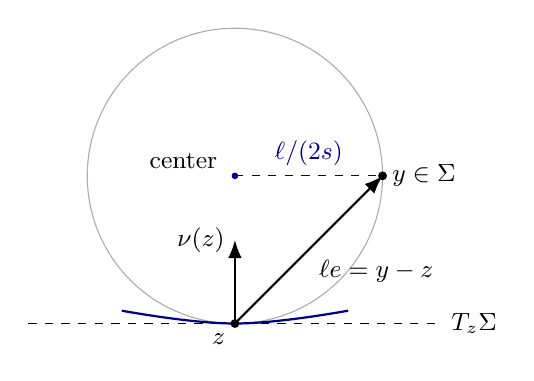
\begin{tikzpicture}[x=1.25cm,y=1.25cm,>=Latex,font=\small]
\draw[gray!65] (0,1.5) circle[radius=1.5];
\draw[dashed] (-2.1,0)--(2.1,0) node[right]{$T_z\Sigma$};
\draw[blue!55!black,thick] (-1.15,.13)..controls(-.55,.025)and(-.2,0)..(0,0)
 ..controls(.2,0)and(.55,.025)..(1.15,.13);
\draw[->,thick] (0,0)--(0,.85) node[left]{$\nu(z)$};
\draw[->,thick] (0,0)--(1.5,1.5) node[midway,below right]{$\ell e=y-z$};
\draw[dashed,blue!55!black] (0,1.5)--(1.5,1.5)
 node[midway,above]{$\ell/(2s)$};
\fill (0,0) circle(1.6pt) node[below left]{$z$};
\fill (1.5,1.5) circle(1.6pt) node[right]{$y\in\Sigma$};
\fill[blue!55!black] (0,1.5) circle(1.2pt);
\node[anchor=east] at(-.08,1.65){center};
\end{tikzpicture}
\caption{The normal-centered circle through two zeros, shown on the
side where $\nu(z)\cdot e=s>0$. Its radius is $\ell/(2s)$, so the
unmodified quotient $\ell/s$ is twice that radius. The blue arc shows
only the local sheet at $z$; the picture asserts neither tangency at
$y$ nor that the circle bounds a zero-free ball. The penalized reach
replaces $1/s$ by $\Gamma(s)$ below.}
\label{fig:reach-tangent-ball}
\end{figure}

We slightly modify this quotient when the chord is almost normal.
The angular factor $\Gamma(s)$ will equal $1/s$ away from $s=1$,
stay uniformly close to $1/s$, and be constant near $1$.
Its constant portion makes the second contact normal to the chord;
this is what will permit the signed transfer in
Proposition~\ref{prop:reach-calculus}.  The transition must also have
small weighted second derivative, so its differentiation costs only
an arbitrarily small error.

Here is a penalty with these properties.  Fix an accuracy
$\eps_1>0$, choose $0<\delta_1<1/10$, then $L>1$, and put
$\delta_2=\delta_1e^{-L}$.  Let $\chi:\R\to[0,1]$
be smooth, nonincreasing, equal to $1$ on $(-\infty,0]$, and equal
to $0$ on $[1,\infty)$.  For $s\ge1-\delta_1$ define
\[
 \Gamma(s)=\frac1{1-\delta_1}
 -\int_{1-\delta_1}^s u^{-2}
   \chi\!\left(\frac{\log(\delta_1/(1-u))}{L}\right)\,\dd u,
\]
and set $\Gamma(s)=s^{-1}$ below $1-\delta_1$.  The integrand is
understood as zero near $u=1$.  This gives a smooth function on
$(0,1]$, constant, with value $G_1$, for $s\ge1-\delta_2$.
Direct differentiation gives
\begin{equation}\label{eq:reach-penalty}
 \begin{gathered}
 s^{-1}\le\Gamma(s)\le(1+C\delta_1)s^{-1},\qquad
 1\le G_1\le\Gamma(s),\\
 -(1-\delta_1)^{-2}\le\Gamma'(s)\le0,\qquad
 0\le(1-s)\Gamma''(s)\le
 \frac{2\delta_1}{(1-\delta_1)^3}
 +\frac{\|\chi'\|_\infty}{L(1-\delta_1)^2}
 \le\eps_1
 \quad(s\ge1-\delta_1).
 \end{gathered}
\end{equation}
The last inequality is achieved by first decreasing $\delta_1$ and
then increasing $L$.  Thus both $G_1-1$ and $\eps_1$ can be prescribed
arbitrarily small.  All choices are made before any large reach or
exhaustion limit.

On $\Sigma_{\rm reg}$ define
\begin{equation}\label{eq:reach-definition}
 d(z)=\inf_{y\in\Sigma\setminus\{z\}}\ell\Gamma(s),\qquad
 \ell=|y-z|,\quad e=\frac{y-z}{\ell},\quad
 s=|\nu(z)\cdot e|.
\end{equation}
A competitor with $s=0$ has value $+\infty$.
An \emph{active contact} is a competitor attaining this infimum, or a
limiting diagonal competitor attaining it as the second point approaches
the base.  The proof of Proposition~\ref{prop:reach-calculus} will show
that one of these alternatives always realizes the infimum.

\begin{lemma}[Elementary chord bounds]\label{lem:reach-small-defect}
The function $d$ is finite and positive on $\Sigma_{\rm reg}$.
At every such point, writing $\lambda_i$ for the eigenvalues of $A$,
\begin{equation}\label{eq:reach-elementary}
 d\max_i|\lambda_i|\le2,
 \qquad |(y-z)\cdot\nu(z)|\le C_\Gamma |y-z|^2/d(z)
 \quad(y\in\Sigma).
\end{equation}
For each $J<\infty$ there is a uniform $\delta(J)>0$ such that
$v(z)=0$ and $D(z)<\delta(J)$ imply $d(z)>J$.
Moreover, at every regular base there are zero-free open balls tangent
at that base on both normal sides, of radius $c_\Gamma d(z)$.
\end{lemma}

\begin{proof}
Local smooth graph representation bounds the quotients
$|\nu(z)\cdot(y-z)|/|y-z|^2$ for nearby zeros; competitors outside a
fixed small ball have a positive lower bound because $\Gamma\ge1$.
This proves positivity.  If every zero lay in the tangent plane at
$z$, phase decay \eqref{eq:phase-decay} would bound the energy by
$C e^{-c\dist(x,T_z\Sigma)}$, giving finite density.  Thus a finite
competitor exists.  A signed unit geodesic tangent to a principal
direction gives
$\ell/s\to2/|\lambda_i|$ whenever $\lambda_i\ne0$, proving the first
inequality.  The second uses the \emph{upper} penalty bound:
$d\le\ell\Gamma(s)\le C_\Gamma\ell/s$.

If $D(z_j)\to0$, the translated, rotated fields $U$ converge smoothly
on every fixed ball to $x_n$, by \eqref{eq:diffuse-local} and the
equation.  In $B_{4J}$ all zeros are therefore one graph whose
curvature and slope tend to zero.  A competitor of value at most
$J$ has $\ell\le J$; on this graph $s\le o(1)\ell$, whereas
$\ell\Gamma(s)\ge\ell/s$.  This is impossible, also for competitors
converging to the diagonal.  The contradiction formulation proves
uniformity of the threshold.  Finally, the second inequality in
\eqref{eq:reach-elementary} excludes zeros from each ball
$B_{c_\Gamma d}(z\pm c_\Gamma d\nu)$ when $c_\Gamma$ is sufficiently
small: a point in either ball has
$|\nu\cdot(y-z)|>|y-z|^2/(2c_\Gamma d)$.
\end{proof}

\begin{remark}[Jointly injective ordinary tubes]\label{rem:reach-ordinary-tube}
The elementary chord inequality also gives the ordinary tube used
in the final packing argument.  If $d(z)>L$, choose
$0<c<\min\{1/(2C_\Gamma),1/2\}$.  For $0<|t|<cL$ and every other zero $y$,
\[
 |z+t\nu(z)-y|^2-t^2
 =|y-z|^2-2t\nu(z)\cdot(y-z)
 \ge(1-2cC_\Gamma)|y-z|^2>0.
\]
Thus $z$ is the unique nearest zero to $z+t\nu(z)$.  Normal tubes
over all bases with $d>L$ are therefore jointly injective in this
range, on both sides.  The curvature bound
$\max|\lambda_i|\le2/d$ implies
$\det(\Id+tA)\ge(1-2c)^m>0$.  Consequently any such bases in
$B_{2R}$ have area at most $C R^{m+1}/L$ when $L\le R$, by integrating
the positive Jacobian over both normal sides and
comparing the resulting tube volume to $|B_{3R}|$.
\end{remark}

\subsection{A bounded density window with delayed monotonicity}

A long reach confines nearby zeros to a thin slab.  We use that
confinement to limit the increase of energy density between successive
radii.  The resulting estimate involves the density at a larger radius,
so its discrete iteration must retain that delay.

\begin{lemma}[A fixed density bound near the reach scale]\label{lem:reach-density-window}
There are fixed $C,c>0$ and a fixed density bound $K_0<\infty$
such that, if $d=d(z)$ is sufficiently large, then
\begin{equation}\label{eq:C1}
 h=d\exp\{-C\sqrt{\log(K(d)+1)}\},\qquad M_h(z)\le K_0.
\end{equation}
The constant $C$ can be increased without invalidating the conclusion.
In particular $h\ge d^{1-o(1)}$, uniformly as $d\to\infty$.
\end{lemma}

\begin{proof}
\emph{Slab confinement and one-step density control.}
Translate $z$ to $0$ and take $\nu(z)=e_n$.  By
\eqref{eq:reach-elementary}, the zeros in $B_{3R}$ lie in
$|x_n|\le C R^2/d$.  With $\mathbb S=e(v)\Id-\nabla v\otimes\nabla v$,
the stress tensor identity $\operatorname{div}\mathbb S=0$, tested
against $x_ne_n\zeta^2$, gives
\[
 \int\zeta^2\mathbb S_{nn}
 =-2\int x_n\zeta\,\mathbb S e_n\cdot\nabla\zeta.
\]
The identities $\nabla v=qp/\sqrt2$ and
$e(v)=q^2(1+|p|^2)/4$ show
$\mathbb S_{nn}\ge c q^2(1-p_n^2)$ and
$|\mathbb S e_n|^2\le Cq^2\mathbb S_{nn}$.
Young's inequality, with a cutoff equal to one on $B_R$ and
supported on $B_{2R}$, consequently proves
\[
 \int_{B_R}q^2(1-p_n^2)
 \le C\int_{B_{2R}}q^2(x_n/R)^2.
\]
On the part of $B_{2R}$ with
$|x_n|>CR^2/d+\sqrt R$, every zero either lies outside $B_{3R}$
or has the confined height, so its distance is at least $c\sqrt R$.
Phase decay controls the energy there by $C R^n e^{-c\sqrt R}$.
Elsewhere $(x_n/R)^2\le C((R/d)^2+R^{-1})$.

In the monotonicity formula between $R/B$ and $R$, with a fixed
$B\ge8$, the discrepancy is bounded by $Cq^2(1-p_n^2)$, and the
squared radial derivative on these annuli by
$C_Bq^2(1-p_n^2+(x_n/R)^2)$.  The preceding estimate, at a fixed
multiple of $R$, therefore gives
\begin{equation}\label{eq:C3}
 0\le M_R(z)-M_{R/B}(z)
 \le C\bigl((R/d)^2+R^{-1}\bigr)M_{BR}(z)
 \qquad(10\le R\le c d).
\end{equation}
The exponentially small remainder was absorbed using $M_R(z)\ge c$
for $R\ge1$.  This uniform lower bound follows from $v(z)=0$,
the uniform first derivative bound, and monotonicity.

\emph{Iterating with the larger-radius term.}
We now retain the delay in \eqref{eq:C3}; replacing $M_{BR}$ by
$M_R$ would give an unjustified recursion.
Set $R_j=dB^{-j}$, $k_j=M_{R_j}(z)$, and
$b_j=C(B^{-2j}+R_j^{-1})$.  Beyond a fixed starting index,
\[
 k_j-k_{j+1}\le b_jk_{j-1}.
\]
Choose $R_{\rm fix}$ and that starting index so $b_j<1/8$ while
$R_j\ge R_{\rm fix}$.  Put
$J=\lceil C_0\sqrt{\log(K(d)+1)}\rceil$.
For sufficiently large $d$, $R_{2J+10}\ge d^{1/2}$, because
$K(d)\le1+Cd$.  Suppose a halving $k_{j+1}<k_j/2$ occurs at some
$j\ge J-2$ before the fixed-scale endpoint.  Then
$k_{j-1}>k_j/(2b_j)>4k_j$, so a halving also occurs at the preceding
index.  Induction propagates this backwards through all indices in
$[\lceil J/2\rceil,J-3]$.  On this interval
$b_i\le C e^{-cJ}$: the $B^{-2i}$ term has this bound, and
$R_i^{-1}\le d^{-1/2}$ is smaller.  Multiplying the preceding lower
growth factors over at least $cJ$ indices gives
$K(d)\ge c\exp(c'J^2)$, contradicting the choice of large $C_0$.
Here all $k_j$ before the endpoint are bounded below by the same
positive constant.  Thus no such halving occurs.

It follows that $k_{j-1}\le2k_j$ for $j\ge J$ up to that endpoint,
and hence $k_{j+1}\ge(1-2b_j)k_j$.  The sum of $b_j$ on this
range is uniformly bounded: the first terms form a geometric series,
and the $R_j^{-1}$ terms form a reversed geometric series ending at
a fixed radius.  The product of $(1-2b_j)^{-1}$ is therefore bounded.
At the last index $M_{R_j}$ has a uniform bound from the bounded
energy integrand.  Consequently $k_J\le K_0$ with fixed $K_0$.
Taking $C$ large enough in \eqref{eq:C1} makes $h\le R_J$;
monotonicity completes the proof.
\end{proof}

\subsection{A bounded positive barrier for the normal operator}

The profile error on either side of an isolated zero sheet vanishes
on that sheet.  To compare this error with its forcing we need a
positive bounded supersolution for the normal operator.  The following
formula will also apply when the boundary of a later comparison region
is shifted by a fixed amount.

\begin{lemma}[Positive half-line barrier]\label{lem:reach-half-line-barrier}
Let $g(t)=\tanh(t/\sqrt2)$ and $V_g(t)=3g(t)^2-1$.
For each fixed $a_0\in\R$, the function
\begin{equation}\label{eq:reach-half-line-barrier}
 v_{a_0}(t)=g'(t)\left[1+\int_{a_0}^t(g'(s))^{-2}
                         \int_s^\infty g'(r)\,\dd r\,\dd s\right],
 \qquad t\ge a_0,
\end{equation}
satisfies
\[
 (-\partial_t^2+V_g)v_{a_0}=1,\qquad
 0<c_{a_0}\le v_{a_0}\le C_{a_0}.
\]
Every fixed derivative of $v_{a_0}$ is bounded on this half-line.
The constants can be chosen uniformly when $a_0$ varies over a fixed
compact interval.  Translating the independent variable gives the
same assertion for a translated profile and half-line.
\end{lemma}

\begin{proof}
Write $v_{a_0}=g'b$ and use
$(-\partial_t^2+V_g)g'=0$.  Then
\[
 (-\partial_t^2+V_g)(g'b)
 =-\frac{1}{g'}\bigl((g')^2b'\bigr)'=1,
\]
since $(g')^2b'=\int_t^\infty g'(r)\,\dd r$.
Both terms in the bracket in \eqref{eq:reach-half-line-barrier} are
nonnegative, and $g'>0$.  Moreover
$g'(t)\sim2\sqrt2e^{-\sqrt2t}$ and
$\int_t^\infty g'=1-g(t)\sim2e^{-\sqrt2t}$, so
$v_{a_0}(t)\to1/2$ as $t\to\infty$.
Continuity gives the positive lower and finite upper bounds, uniformly
for $a_0$ in a compact interval.  Differentiating the displayed formula
gives a bounded first derivative; the equation and its successive
derivatives give all remaining fixed derivative bounds.
\end{proof}

\subsection{Isolation and the two parity projections}

The density window now gives one graph on the scale $h$.
For reach calculus we need more than its curvature bound: the first
two derivatives of $H$ must be smaller than the scale-invariant
$h^{-3}$ size.  Two projections in the normal variable provide this
gain.  The first uses oddness of the leading curvature forcing; the
second uses the tangential improvement obtained from the first.

\begin{lemma}[An isolated graph and mean-curvature derivatives]\label{lem:reach-isolation}
There are uniform $c,c',C,\gamma>0$ such that, for sufficiently
large $d(z)$ and $h$ in \eqref{eq:C1}, the zero set in $B_{ch}(z)$
is a single graph over $T_z\Sigma$, extending over the tangent disk
of radius $c'h$.  On a smaller concentric portion,
\begin{equation}\label{eq:C2}
 \begin{gathered}
 |A|+h^{1/2}[A]_{C^{1/2}}\le C h^{-1},\qquad
 |\nabla_\Sigma A|\le C h^{-2},\qquad |H|\le C h^{-2},\\
 |\nabla_\Sigma H|+|\nabla_\Sigma^2H|\le C h^{-3-\gamma}.
 \end{gathered}
\end{equation}
The estimates hold uniformly on every inner patch having a fixed
fractional margin from the original chart boundary.  Hölder norms
may be computed in its graph coordinates.
\end{lemma}

\begin{proof}
\emph{One graph and preliminary bounds.}
The fixed bound of Lemma~\ref{lem:reach-density-window} is subcritical
by Theorem~\ref{thm:finite}.  Apply
Corollary~\ref{cor:finite-subcritical}, including its sheeting conclusions,
at radius $h$.  Thus the density used here is the fixed local bound
$K_0$; the contradiction hypothesis still allows unbounded density on
larger scales.
The confinement thickness divided by this radius is $O(h/d)$.
Increasing the fixed constant in \eqref{eq:C1} makes this ratio as
small as required, without changing the density bound.  The resulting
graphs have arbitrarily small fixed slope, the first estimate in
\eqref{eq:C2}, and
\begin{equation}\label{eq:reach-preliminary-H}
 |H|\le C_\iota h^{-2+\iota}\quad\text{for every fixed }\iota>0.
\end{equation}
An additional graph in an inner cylinder would cross the normal line
at $z$ at distance $O(h)$, producing a competitor of value $O(h)$,
contrary to $d/h$ being sufficiently large.  Thus just one sheet
remains in a smaller cylinder.  On fixed windows centered on inner
zeros the solution, in oriented normal coordinates, converges
uniformly and smoothly to $g$.  The lower gradient bound from sheeting
and interior elliptic estimates also give unit-scale bounds on all
fixed orders of graph derivatives.  These statements are uniform in
the centers and solutions, by the stated uniformity of the subcritical
ball input and the usual sequential formulation of compactness.

It remains to strengthen the mean-curvature derivatives and then recover
the large-scale bound on $\nabla_\Sigma A$.  The two projections below
serve different purposes: the first removes the leading odd forcing
from the equation at the zero sheet, and the second uses the resulting
tangential gain to improve the derivatives of $H$.
We prove the derivative improvement; in particular we do not
differentiate \eqref{eq:reach-preliminary-H} at its original scale.
Fix an inner zero as origin.  Let $X(y)$ be its tangent-plane graph
and use Fermi coordinates $X(y)+t\nu(y)$.  Choose a small number
$\epsilon>0$, to be fixed at the end, and write $R_h=h^\epsilon$.
All arguments below take place in a fixed finite sequence of nested
boxes with side lengths fixed fractions of $R_h$, starting inside
$\{|y|_\infty,|t|<R_h\}$.  The much larger $h$-scale chart guarantees
that these coordinates are injective there, have polynomially bounded
unit-scale derivatives of each fixed order, and contain no other
zero.  The distance to $\Sigma$ is comparable to $|t|$ on the boxes.
Consequently
\[
 \varphi(y,t)=v(X(y)+t\nu(y))-g(t)=o(1)
\]
uniformly.  To see uniformity also at unbounded $t$, first choose a
large fixed depth and use phase decay beyond it, then use the fixed
window convergence at shallower depths.  For $|t|$ a fixed fraction
of $R_h$, $\varphi$ and every needed fixed derivative are bounded by
$C h^C e^{-cR_h}$: apply phase decay and unit-scale elliptic estimates
to $v\mp1$, and differentiate the coordinate composition.

We record the interpolation used below.  If a tensor has uniformly
bounded $C^N$ norm on unit balls and $C^{1/2}$ seminorm at most
$Ch^{-3/2}$, its derivatives of orders $1\le k\le30$ are bounded by
$C h^{-5/4}$, by taking $N$ sufficiently large once and for all.
Indeed the standard interpolation exponent of the low seminorm can
be taken arbitrarily close to one for any fixed $k$ by increasing
$N$; subtracting its value at the center removes the constant term.
Applied to the coordinate components of $A$, whose change-of-frame
terms have the same or better bound, this gives
\begin{equation}\label{eq:reach-interpolation}
 |\partial_y^k A|\le C h^{-5/4}\quad(1\le k\le30),\qquad
 |\partial_y^kH|\le C_\epsilon h^{-2+\epsilon}\quad(0\le k\le30).
\end{equation}
For the second assertion use \eqref{eq:reach-preliminary-H} with
$\iota<\epsilon/2$ and interpolate its supremum norm with a
sufficiently high unit-scale derivative bound.  All interpolation
orders are finite and fixed before $h$ tends to infinity.

In these coordinates the equation is exactly
\begin{equation}\label{eq:C4}
 \begin{split}
 (-\Delta_y-\partial_t^2+V_g)\varphi={}&K_tg'+K_t\varphi_t
 +(g_t^{ij}-\delta^{ij})\partial_{ij}\varphi
 +b_t^i\partial_i\varphi-3g\varphi^2-\varphi^3,\\
 V_g={}&3g^2-1,\qquad
 K_t=\tr[A(\Id+tA)^{-1}]\,.
 \end{split}
\end{equation}
Here $g_t^{ij}$ is the inverse tangential metric, and $b_t^i$ is the
first-order coefficient in its Laplace operator.  Neither superscript
nor subscript $t$ denotes differentiation in this display.  Matrix
inversion in $\Id+tA$, the graph metric, and
\eqref{eq:reach-interpolation} give, with derivatives through order
20,
\begin{equation}\label{eq:reach-coefficients}
 \begin{gathered}
 K_t=H-t|A|^2+t^2\tr A^3+O(h^{-4+C\epsilon}),\qquad
 K_t=O(h^{-2+C\epsilon}),\\
 g_t^{ij}-\delta^{ij}=O(h^{-1+C\epsilon}),\qquad
 b_t^i=O(h^{-1+C\epsilon}).
 \end{gathered}
\end{equation}
Every occurrence of $C\epsilon$ in this proof has a bounded absolute
multiplier independent of $\epsilon$.  For example the tangent slope
is $O(h^{-1+\epsilon})$, and the remainder in the first line contains
at least four factors of $A$ and at most a fixed power of $|t|$.
The differentiated remainders obey the same bounds, since each
positive derivative of $A$ is no larger than $O(h^{-1})$.

\emph{A first bound for the profile error.}
Use $v_0$ from Lemma~\ref{lem:reach-half-line-barrier} on $t\ge0$
and its reflection on $t\le0$, separately on the two half-boxes.
The reflected pair need not be differentiable at zero; no full-line
supersolution is asserted.  In each half-box move the metric
and drift terms to the left of
\eqref{eq:C4} and write the nonlinearity as
$(3g\varphi+\varphi^2)\varphi$.  Its coefficient tends uniformly to
zero, so the resulting operator applied to $v_0$ is at least $1/2$.
Comparison is valid after division by this positive supersolution,
which makes the zeroth-order coefficient positive.  For each lateral
or distant normal face, $v_0e^{-c_0\,\text{distance to face}}$ is also
a supersolution when $c_0$ is a sufficiently small fixed number.
The sum of these face barriers and $C h^{-2+C\epsilon}v_0$ dominates
both signs of $\varphi$.  The bottom boundary has $\varphi(y,0)=0$.
Shrinking the box makes all face contributions exponentially small.
Interior elliptic estimates across $t=0$, using the smooth equation,
then give
\begin{equation}\label{eq:reach-phi-first}
 \|\varphi\|_{C^{15}}\le C_\epsilon h^{-2+C\epsilon}.
\end{equation}
The coefficient norms needed for this bootstrap are uniform by
\eqref{eq:reach-coefficients}; the nonlinearity is smooth and has
already been bounded in supremum norm.

\emph{The inverse on the complement of the translation mode.}
The positive barrier controlled the full profile error.  The next
estimate separates its translation mode from the remaining normal
modes, where a spectral gap is available.
Let $L_t=-\partial_t^2+V_g$.  It has kernel spanned by $g'$ and
a fixed spectral gap $\lambda>0$ on its $L^2(\R)$ orthogonal
complement.  One elementary justification is the ground-state
factorization of its quadratic form, simplicity of the positive
zero mode, and compactness on bounded intervals together with
$V_g\to2$ at infinity; a Rayleigh sequence tending to zero could
neither escape to infinity nor stay orthogonal to the kernel.
Let $P_\perp$ be this projection.  For
\[
 (-\Delta_y+L_t)w=P_\perp F,\qquad P_\perp w=w,
\]
the regularized $L_t^2$ norm of each $y$-derivative of $w$ is a
subsolution for $-\Delta_y+\lambda$, with source the corresponding
norm of $F$.  This follows by differentiating the squared norm,
using $\langle L_tw,w\rangle\ge\lambda\|w\|_2^2$ and
Cauchy--Schwarz, and then letting the regularization vanish.
Comparison with the constant source bound plus decaying face
barriers controls these norms on each smaller $y$-box, with an
exponentially small multiple of their boundary bound.  Commuting two
additional $y$-derivatives and using the equation gives the same
bound in $H_t^2$, since
$\|w\|_{H^2}\le C(\|L_tw\|_2+\|w\|_2)$.
Thus source derivatives through order $j+2$ control the value at
$t=0$ and its $y$-derivatives through order $j$.
This assertion applies separately to even and odd functions of $t$,
because both the operator and $P_\perp$ preserve parity.  It applies
also to a range of strictly positive derivative orders: no estimate
of the undifferentiated source is needed to estimate a differentiated
equation.  Polynomial boundary bounds suffice in every use here.

\emph{The whole-line equation and the first parity projection.}
Choose an even cutoff $\chi_h(t)$, equal to one on an inner normal
interval and supported in a slightly larger interval inside the box,
with derivatives supported where $|t|$ is comparable to $R_h$.  Put
$\Phi=\chi_h\varphi$.  If $E_{\rm raw}$ denotes the right side of
\eqref{eq:C4} minus $Hg'$, the exact equation on the whole normal line is
\[
 (-\Delta_y+L_t)\Phi=Hg'+E_{\rm full},\qquad
 E_{\rm full}=\chi_h E_{\rm raw}+(\chi_h-1)Hg'
                  -2\chi_h'\varphi_t-\chi_h''\varphi.
\]
The kernel tail $(\chi_h-1)Hg'$ and the two commutators, together with
all their needed $y$-derivatives, are $O(h^{-N})$ for every fixed $N$.
For the tail this follows from the preliminary derivatives of $H$ and
the exponential decay of $g'$; for the commutators it follows from the
normal-edge estimates.  Restoring the cutoff leading term
$-\chi_h t|A|^2g'$ to the whole-line odd function $-t|A|^2g'$ costs
another error of the same order.  We henceforth write $\varphi$ for
$\Phi$, and $E$ for $E_{\rm full}$.  Write
\[
 \varphi=u_0(y)g'(t)+\varphi^\perp(y,t),\qquad
 (-\Delta_y+L_t)\varphi=H(y)g'(t)+E(y,t).
\]
We normalize kernel coefficients by $\int(g')^2$.
From \eqref{eq:reach-coefficients} and \eqref{eq:reach-phi-first},
in $L_t^2$ with $y$-derivatives through order 11,
\begin{equation}\label{eq:reach-first-parity}
 E=-t|A|^2g'+O(h^{-3+C\epsilon}),\qquad
 E^{\rm even}=O(h^{-3+C\epsilon}).
\end{equation}
Here $t^2\tr A^3g'$ has size $h^{-3+C\epsilon}$, every metric
error is a coefficient of size $h^{-1+C\epsilon}$ times a derivative
of $\varphi$ of size $h^{-2+C\epsilon}$, and the normal-drift and
nonlinear errors have size $h^{-4+C\epsilon}$.

The inverse estimate for the even orthogonal component, followed by
evaluation at $t=0$, bounds $\varphi^\perp(y,0)$ and its derivatives
through order 9 by $C h^{-3+C\epsilon}$; the odd component vanishes
there.  Since $\varphi(y,0)=0$, the same bound holds for $u_0$.
The kernel equation
\begin{equation}\label{eq:reach-kernel}
 -\Delta_yu_0=H+E_0
\end{equation}
therefore bounds $H$ and its derivatives through order 7 by
$C h^{-3+C\epsilon}$.  In addition, positive $y$-derivatives of
$-t|A|^2g'$ gain $h^{-1/4}$ over its $h^{-2}$ bound by
\eqref{eq:reach-interpolation}; derivatives of the remainder in
\eqref{eq:reach-first-parity} are already smaller.  Applying the
inverse estimate to the entire orthogonal component consequently gives
\begin{equation}\label{eq:reach-positive-phi}
 \|\partial_y^k\varphi\|_{L_t^2}
 \le C h^{-2-1/4+C\epsilon},\qquad1\le k\le8.
\end{equation}
For these $L_t^2$ bounds no loss of two derivative orders is required;
the already controlled derivatives of $u_0$ cover the kernel term.

The first projection has now bounded the kernel coefficient through
nine tangential derivatives and $H$ through seven.  The full orthogonal
equation has also supplied the gain in \eqref{eq:reach-positive-phi}
without losing derivative orders.  We use that gain in a second even
projection; no eighth derivative of $H$ is required, because $P_\perp$
annihilates $Hg'$.

\emph{The second parity projection.}
Return to \eqref{eq:C4}.  Positive derivatives through order 6 of
the even part of $E$ now obey
\begin{equation}\label{eq:reach-second-parity}
 \|\partial_y^kE^{\rm even}\|_{L_t^2}
 \le C h^{-3-1/4+C\epsilon},\qquad1\le k\le6.
\end{equation}
Indeed the odd term $-t|A|^2g'$ still contributes nothing; a positive
derivative of $\tr A^3$ contains a factor bounded by $h^{-5/4}$;
every horizontal metric or drift error contains at least one positive
$y$-derivative of $\varphi$, so \eqref{eq:reach-positive-phi} applies
up to order 8.  If derivatives instead fall on its coefficient, that
coefficient remains $O(h^{-1+C\epsilon})$ and the same estimate
applies to the positive derivative already present on $\varphi$.
The normal drift and nonlinear terms remain $O(h^{-4+C\epsilon})$
in these norms.  This accounts for all terms, including products of
derivatives and the superpolynomially small cutoff errors.

Apply the even orthogonal inverse once more.  Its value at zero and
the zero condition give
$|\partial_y^ku_0|\le C h^{-3-1/4+C\epsilon}$ for $1\le k\le4$.
Equation~\eqref{eq:reach-kernel} gives the same estimate for
$\partial_yH$ and $\partial_y^2H$.  Choose $\epsilon$ so small that
every fixed exponent loss $C\epsilon$ above is less than $1/8$;
decreasing the resulting gain if necessary gives $\gamma>0$.
Covariant derivatives have the asserted bounds as well: the coordinate
connection is bounded and its extra terms multiply already controlled
first derivatives of $H$.

\emph{Recovering the large-scale curvature derivative.}
The improved mean-curvature derivatives are now in hand.  Rescale
the original graph disk by $h^{-1}$.  Its existing
$C^{2,1/2}$ bound is uniform, and the rescaled mean curvature $hH$
has uniformly bounded $C^{1,1}$ norm, since its first and second
derivatives scale by $h^2$ and $h^3$, respectively.  Differentiate
the prescribed mean-curvature graph equation once and apply interior
Schauder estimates.  The rescaled graph has a uniform third derivative
bound, giving $|\nabla_\Sigma A|\le Ch^{-2}$ in original variables.
All boxes used above have a fixed total fractional shrinkage and all
derivative orders were fixed in advance.  Repeating at each inner
center proves the uniform inner-window assertion.
\end{proof}
\subsection{One-sided trace improvement from a tangent phase ball}

The isolated chart controls the base point of a reach contact.  Its
second point need not lie in that chart, so it requires an estimate
whose sole geometric input is a zero-free tangent ball.  The sign of
the resulting trace bound matters: only positive mean curvature at the
receiving point will enter the upper reach inequality.

\begin{lemma}[One-sided improvement at a tangent phase ball]\label{lem:reach-phase-ball}
There are uniform $r_0,C,\gamma>0$ with the following property.
If an open ball of radius $r\ge r_0$ is disjoint from $\Sigma$ and
its boundary contains $x\in\Sigma$, and $N$ is its inward normal at
$x$, then
\begin{equation}\label{eq:C5}
 x\in\Sigma_{\rm reg},\qquad D(x)\le C/r,
 \qquad a(x)\le C/r,\qquad H_N(x)\le Cr^{-1-\gamma}.
\end{equation}
After changing the sign of $v$ so that it is positive inside the
ball, along the inward radius one also has
\begin{equation}\label{eq:C6}
 U(x+sN)\ge s-C(1+s)/r\qquad(0\le s\le\log r).
\end{equation}
Only the last curvature estimate is one-sided; no absolute-value
improvement for $H_N$ is asserted.
\end{lemma}

\begin{proof}
\emph{Comparison along the inward radius.}
Let $s$ denote inward depth in the annulus $0<s<Q=\sqrt r$.
The nonnegative function
\[
 w(s)=g'(s)\int_0^s(g'(t))^{-2}
                    \int_t^\infty(g'(u))^2\,\dd u\,\dd t
\]
has $w(0)=0$, $(-\partial_s^2+V_g)w=g'$, and
$|w|+|w'|\le C(1+s)g'$.  Thus $v_*=g-C_0w/r$, with a sufficiently
large fixed $C_0$, is positive on the annulus and satisfies
$\Delta v_*+v_*-v_*^3>0$.  Indeed the linear correction contributes
$C_0g'/r$, the inward radial drift is
$-(n-1)v_*'/(r-s)$, and the quadratic correction is bounded by
$C r^{-2}(1+s)^2(g')^2=o(r^{-1}g')$ uniformly on $[0,Q]$.
Multiplication by $1-e^{-cQ}$, with a sufficiently small fixed
$c>0$, keeps a strict subsolution and makes its value less than $v$
on the inner boundary, by phase decay.  On the outer boundary it
vanishes.  Sliding its amplitude from a small positive number to one
proves comparison.  To justify the start, $v>0$ in the compact
annulus and the Hopf boundary estimate applies at any outer zero;
these and compactness bound the quotient from below.  At a first
contact a strict subsolution cannot touch in the interior, and the
Hopf comparison excludes an outer boundary obstruction.  Smaller
amplitudes remain strict subsolutions: writing
$\mathcal F(w)=\Delta w+w-w^3$, one has
$\mathcal F(av_*)=a\mathcal F(v_*)+(a-a^3)v_*^3>0$ for $0<a\le1$.

Inverting $g$ on $0\le s\le\log r$ proves \eqref{eq:C6}:
the correction is bounded by $C(1+s)g'(s)/r$, and the extra
$e^{-c\sqrt r}$ term is smaller after division by $g'(s)$ on that
range.  Differentiation at the contact point gives
$\partial_Nv(x)\ge g'(0)-C/r>0$.  Thus $x$ is regular, $N=\nu$
after the sign choice, and $D(x)\le C/r$.  The tangent ball gives
the principal-curvature lower bound $\lambda_i(A_N)\ge-1/r$.
The zero-level identity $H_N=\partial_ND/(2|p|^2)$ and
\eqref{eq:diffuse-local} give $|H_N|\le CD\le C/r$.
Summing the principal curvatures then bounds each one from above by
$C/r$, proving the full curvature estimate in \eqref{eq:C5}.

\emph{Separating the even source from the boundary contribution.}
The comparison has established regularity and the $r^{-1}$ bounds.
To improve only the upper trace, place $x=0$, $N=e_n$, and use the
ambient vertical coordinate $s$.  Work in $B_P$ with
$P=\alpha\log r$, where $\alpha>0$ is fixed sufficiently small at
the end.  The differentiated diffuse estimates give, for every
needed fixed order $k$,
\[
 \|D\|_{C^k(B_P)}\le C_k r^{-1+C\alpha},\qquad
 \|T\|_{C^k(B_P)}+\|U-s\|_{C^k(B_P)}
 \le C_k r^{-1/2+C\alpha}.
\]
These follow by applying unit-ball derivative estimates and the
exponential comparison for $D$ along chains from $0$; integration
of $T$ gives the estimate on $U-s$.  The multipliers of $\alpha$
are fixed independently of small $\alpha$.  The identity
$\nabla_pT=-T^2-\nabla^2D/2$ further gives
$\partial_sT=O(r^{-1+C\alpha})$: the replacement of $p$ by $e_n$
has error $|p-e_n||\nabla T|=O(r^{-1+C\alpha})$.

Set $F=G(s)D$.  Conjugating the defect equation and replacing $vp$
by $g(s)e_n$ and $q|p|^2$ by $G(s)$ yields
\begin{equation}\label{eq:reach-ball-conjugation}
 (-\Delta+2-G(s))F
 =2G(s)|T(x',0)|^2+\mathcal E,
 \qquad\|\mathcal E\|_\infty\le Cr^{-3/2+C\alpha}.
\end{equation}
For completeness, each replacement in the drift or potential
multiplies a coefficient of size $r^{-1/2+C\alpha}$ by $D$ or
$\nabla D$ of size $r^{-1+C\alpha}$.  Replacing
$|T(x',s)|^2$ by $|T(x',0)|^2$ has the same order, since
$|T|=O(r^{-1/2+C\alpha})$, $\partial_sT=O(r^{-1+C\alpha})$,
and $|s|\le P$.  Logarithmic factors are absorbed by increasing
the fixed multiplier of $\alpha$.

Solve the Dirichlet problem on $B_P$ by linearity.  The solution
with source $2G|T(x',0)|^2$ and zero boundary is even in $s$ and
nonnegative.  The zero-boundary solution for $\mathcal E$ has
interior $C^1$ norm at most $Cr^{-3/2+C\alpha}$, since the potential
$2-G$ is at least one.  The remaining homogeneous solution is
$u_++u_-$, both nonnegative, with boundary values $F$ on the upper
and lower hemispheres, respectively, and zero on the other one.
Their harmless equatorial boundary discontinuity is interpreted by
bounded Dirichlet solutions; it does not affect interior estimates.
Reflection and the maximum principle in the upper half-ball give
$\partial_su_-(0)\le0$; local Harnack and derivative estimates give
$|\partial_su_+(0)|\le Cu_+(0)$.

At $x_*=(0,P/2)$, positivity of the source solution implies
\[
 u_+(x_*)\le F(x_*)+Cr^{-3/2+C\alpha}
 \le C(1+P)r^{-1}G(P/2)+Cr^{-3/2+C\alpha}.
\]
For the last inequality integrate $D\le2(1-\partial_sU)$ along
$[0,P/2+1]$, use \eqref{eq:C6}, and apply unit-scale Harnack to $D$
to pass from the integral to its value at $P/2$.  This use is valid
for $\alpha<1$, so the interval lies in the range of \eqref{eq:C6}.

\emph{Suppressing the upper boundary contribution.}
Only $u_+$ can contribute a positive leading normal derivative at the
origin.  Its value at $x_*$ is small by the inward comparison; we
now transfer that gain to the origin with explicit Poisson bounds.
Write $A_\partial=\int_{\partial B_P\cap\{s>0\}}F\,\dd S$.
Comparison with potentials one and two gives
\begin{equation}\label{eq:reach-poisson}
 u_+(0)\le CP^C e^{-P}A_\partial,
 \qquad
 u_+(x_*)\ge c_\zeta
 e^{-(\sqrt2+\zeta)\sqrt5 P/2}A_\partial
 \quad(\zeta>0).
\end{equation}
For the first inequality, the Poisson density at the center for
$-\Delta+1$ is constant on the sphere.  The spherical average of
$e^{x\cdot\theta}$ shows that its size is at most $CP^Ce^{-P}$.
The solution for potential $2-G\ge1$ is smaller.  For the second,
the solution for potential $2-G\le2$ is larger than that for
$-\Delta+2$.  Its Dirichlet Poisson density at any upper-hemisphere
point $\xi$ is at least
$c_\zeta e^{-(\sqrt2+\zeta)|x_*-\xi|}$.  Here are quantitative
details of this last bound.  Start the Dirichlet Green function a
fixed distance from $x_*$, with a fixed positive lower bound obtained
from a fixed-radius ball.  Along the segment towards $\xi$ insert
a cylinder of fixed large cross-sectional radius, chosen so that
$\sqrt{2+\lambda_1}<\sqrt2+\zeta$.  Its first transverse
Dirichlet mode times the longitudinal hyperbolic-sine solution
propagates the lower bound with that exponential rate.  Stop a fixed
distance before $\xi$.  Such a cylinder fits in $B_P$ except for
fixed initial and final portions: $x_*$ is at distance $P/2$ from
the boundary and the incidence angle at $\xi$ has a cosine bounded
below uniformly.  Harnack on those fixed portions and a tangent-ball
barrier at $\xi$ transfer the bound to the inward normal derivative.
All constants depend on $\zeta$ but not $P$.  Finally
$|x_*-\xi|\le\sqrt5 P/2$, proving \eqref{eq:reach-poisson}.

Combining the two bounds with $G(P/2)\le Ce^{-\sqrt2 P/2}$ gives
\[
 u_+(0)\le CP^C r^{-1}
 e^{[(\sqrt2+\zeta)\sqrt5/2-1-\sqrt2/2]P}
 +CP^C r^{-3/2+C\alpha}
 e^{[(\sqrt2+\zeta)\sqrt5/2-1]P}.
\]
Since $\sqrt{10}/2-1-\sqrt2/2<0$, choose $\zeta$ so the first
exponent is negative, then choose $\alpha>0$ so the second term
still has a power better than $r^{-1}$.  Polynomial factors in $P$
can be absorbed by slightly decreasing a resulting gain $\gamma>0$.
The source solution has zero derivative at $0$, the lower-hemisphere
solution has nonpositive derivative there, and the error solution is
smaller still.  Thus $F_s(0)\le Cr^{-1-\gamma}$.  Since
$G(0)=1$, $G'(0)=0$, and $|p(0)|^2=1-O(r^{-1})$, the zero-level
identity for $H_N$ proves \eqref{eq:C5}.
\end{proof}

\subsection{The weak reach inequality and transfer of positive charge}

We now combine the base estimates with the tangent-ball bound.  At an
active contact on the plateau of the penalty, the second point will be
called the \emph{receiving foot}.
The proposition distinguishes these contact types because only plateau
contacts retain a mean-curvature term at that foot.  It also specifies
the direction and multiplicity of the area change needed when that
positive term is integrated.

\begin{proposition}[Weak reach inequality and positive-foot transfer]\label{prop:reach-calculus}
Given $\eta_0>0$, the penalty parameters can be chosen, in the order
specified above, so that the following holds for all sufficiently
large $d$.  The function $d$ is locally semiconcave on
$\Sigma_{\rm reg}$, and the singular part of its distributional
surface Laplacian is nonpositive.  Almost everywhere,
\begin{equation}\label{eq:C7}
 |\nabla_\Sigma d|\le
 C_\Gamma\exp\{C_\Gamma\sqrt{\log(K(d)+1)}\}.
\end{equation}
At an active non-plateau or diagonal contact,
\begin{equation}\label{eq:C8}
 \Delta_\Sigma d\le(1+\eta_0+C_\Gamma d^{-\gamma})a^2d
                  +B\,\frac{|\nabla_\Sigma d|^2}{d},
 \qquad B\le1+C_\Gamma d^{-\gamma}.
\end{equation}
If $ad$ is sufficiently small, the same bound can be used with
$B\le\eta_0+C_\Gamma ad+C_\Gamma d^{-\gamma}$, and then
$|\nabla_\Sigma d|\ge c_\Gamma>0$.
At an active plateau contact, meaning $s\ge1-\delta_2$, one has
\begin{equation}\label{eq:C9}
 \Delta_\Sigma d\le
 G_1\bigl(|H(z)|+H_{N_y}(y)_+\bigr)
 +\eta_0\frac{|\nabla_\Sigma d|^2}{d},\qquad N_y=-e.
\end{equation}
For any measurable choice of such contacts, the positive foot charge
can be transferred to $y$ with multiplicity at most one and area factor
\begin{equation}\label{eq:C10}
 J_{y\to z}=
 \frac{|\det(\Id+\ell A_{N_y}(y))|}{s}\le C_\Gamma,
 \qquad d(y)\le d(z)=G_1\ell,
 \qquad a(y)+D(y)\le C_\Gamma/d(z).
\end{equation}
More precisely, $J_{y\to z}\le1+C\delta_2+C a(y)\ell$ whenever
$a(y)\ell$ is bounded by a sufficiently small fixed constant.  The
constants and the large-reach threshold are fixed before any later
defect threshold, collar scale, or exhaustion radius is chosen.
\end{proposition}

\begin{proof}
\emph{Semiconcavity, including diagonal competitors.}
We first justify the weak interpretation, independently of the
differentiations to follow.  On a compact regular coordinate patch
there are uniform bounds $0<c\le d\le C$: local graph curvature
gives the lower bound, and one fixed off-diagonal positive-angle
competitor gives the upper bound after shrinking the patch.
Relevant competitors of value at most $2C$ have bounded length.
Those of length at least $\varepsilon>0$ have angle
$s\ge\varepsilon/(2C)$, by $\Gamma\ge1/s$.  With the second foot
fixed, these are smooth branches in the base variable, uniformly
bounded in $C^2$; no regularity of the second foot is needed here.

For shorter chords the second point is on the same regular local
graph.  In coordinates $X(u)$ write it as $X(u+t\omega)$, with
$|\omega|=1$ and $t$ small.  Such chords use $\Gamma=1/s$.
The reciprocal branch is
\[
 \frac{|\nu(u)\cdot[X(u+t\omega)-X(u)]|}
 {|X(u+t\omega)-X(u)|^2}.
\]
Both numerator before absolute value and denominator vanish to
second order in $t$, since $DX$ is tangent.  Cancelling $t^2$ by
the integral Taylor formula gives a $C^2$ function through $t=0$,
uniformly in the compact direction parameter.  On relevant branches
its absolute value is bounded below by $1/(2C)$, so a smooth sign
can be chosen and taking its reciprocal preserves the uniform
$C^2$ bound.  The diagonal limits are legitimate upper branches
for $d$, since they are limits of competitors.  Compactness of the
remaining parameter sets shows that every minimizing sequence
has either an off-diagonal or a diagonal realizing parameter and
that $d$ is the infimum of a family with locally uniform upper
Hessian bound.  Subtracting the corresponding fixed quadratic
function makes each branch concave and hence also their infimum
concave.  This proves local semiconcavity.

At almost every point there is an Alexandrov second-order expansion.
At such a point any smooth active upper branch has the same first
derivative and an upper bound for the Hessian of $d$.  Its trace
therefore bounds the absolutely continuous Laplacian.  The singular
part is a nonpositive measure by semiconcavity, in coordinates and
therefore for the surface Laplacian as well.  It suffices to compute
the following upper touching branches.

The weak interpretation is now established.  We next compute smooth
upper touching branches, treating the unmodified penalty, diagonal
limits, and the transition to the plateau in that order.  The final
step will transfer the positive plateau contribution to its receiving
foot.

\emph{A tangent phase ball at every second foot.}
For an off-diagonal contact choose $N=\pm\nu(z)$ so $N\cdot e=s>0$.
The open region
\[
 \{z+\ell'e':N\cdot e'>0,\ \ell'\Gamma(N\cdot e')<d\}
\]
contains no zeros.  After translation, rotation, and division by $d$,
its boundary is a fixed smooth embedded compact radial surface.  Near
the origin it agrees with the sphere $|x|^2=x_n$, because there
$\Gamma(s)=1/s$.  On the remainder it is the smooth positive radial
graph $1/\Gamma$.  It has an inward rolling ball of a fixed positive
radius $c_\Gamma$: local $C^2$ graph bounds supply the balls near
each point, and compactness and embeddedness allow a uniform
decrease so those balls avoid the rest of the boundary.  Hence at
the second foot $y$ there is a zero-free tangent ball of radius
$c_\Gamma d$.  Lemma~\ref{lem:reach-phase-ball} shows that the foot
is regular, $a(y)+D(y)\le C_\Gamma/d$, and its inward trace satisfies
$H_{N_y}(y)\le C_\Gamma d^{-1-\gamma}$.

\emph{Off-diagonal contacts with the unmodified penalty.}
First suppose $s\le1-\delta_1$, so $\Gamma=1/s$.  Write
$r=d/2$, $b=e-sN$, and $M=\Id+rA_N$.  Then $\ell=2rs$ and the
inward normal at the second foot is $N_y=N-2se$.
Reflect an orthonormal frame $v_i$ of $T_z\Sigma$ across $e^\perp$
to obtain $v_i'=v_i-2(e\cdot v_i)e$ in $T_y\Sigma$.  Move $z$ and
$y$ on the respective geodesics with these initial velocities.
The resulting chord branches touch $d$ from above.  First and second
differentiation gives
\begin{equation}\label{eq:C11}
 \begin{split}
 \nabla_\Sigma r={}&-Mb/s,\\
 \Delta_\Sigma d\le{}&a^2d+
 \left(2-\frac2{1+r\max_i|\lambda_i|}\right)
             \frac{|\nabla_\Sigma d|^2}{d}\\
 &+\frac{H_{N_y}(y)-(1-2s^2)H_N(z)
                -\ell b\cdot\nabla_\Sigma H_N(z)}{s^2}.
 \end{split}
\end{equation}
Here is the algebra, including the factor of the gradient term.
Put $w=y-z$ and $w_i=v_i'-v_i=-2(e\cdot v_i)e$ and differentiate
$|w|^2/2-rN\cdot w$, which vanishes at contact and is nonnegative
for a competitor.  The summed second derivative bounds
$(\Delta r)s\ell$ by
\[
 \begin{split}
 &\sum_i|w_i|^2+(w-rN)\cdot(-H_{N_y}N_y+H_NN)
 -2r\sum_iw_i\cdot A_Nv_i\\
 &\hspace{8mm}-rw\cdot(\nabla H_N-a^2N)
 -2\sum_i r_i\bigl(w_i\cdot N+w\cdot A_Nv_i\bigr).
 \end{split}
\]
Use $w-rN=-rN_y$ and the first derivative identity.
The algebraic terms besides $a^2$ and the traces reduce to
$4s^2|\nabla r|^2+4s b\cdot\nabla r$.  By
\eqref{eq:reach-elementary}, $0\le M\le
(1+r\max_i|\lambda_i|)\Id$, so
\[
 b\cdot\nabla r=-b\cdot Mb/s
 \le-\frac{s|\nabla r|^2}{1+r\max_i|\lambda_i|}.
\]
Dividing the preceding second derivative expression by $rs^2$
therefore gives exactly \eqref{eq:C11}.  The identity
$\Delta_\Sigma N=\nabla_\Sigma H_N-a^2N$ fixes all trace signs.

We bound its last quotient uniformly, including almost tangential
contacts.  Choose a small fixed $\gamma'>0$ compared with the gains
in Lemmas~\ref{lem:reach-isolation} and \ref{lem:reach-phase-ball}.
If $s\ge d^{-\gamma'}$, the second-foot upper trace, the base bounds
$|H|\le Ch^{-2}$ and $|\nabla H|\le Ch^{-3-\gamma}$, and
$h=d^{1-o(1)}$ bound that quotient above by
$C_\Gamma d^{-1-\gamma''}$ for some fixed $\gamma''>0$.
If $s<d^{-\gamma'}$, then $\ell=ds$ lies inside the isolated graph.
The two normal orientations agree by continuation there.  In its
tangent-plane coordinates the displacement is exactly $\ell b$;
Taylor's formula gives
\[
 H_{N_y}(y)-H_N(z)-\ell b\cdot\nabla H_N(z)
 =O(\ell^2h^{-3-\gamma}).
\]
The coordinate Hessian obeys this bound as well, since its connection
correction multiplies the already controlled gradient.  Dividing by
$s^2$ and adding $2H_N(z)$ proves the same upper error after possibly
decreasing $\gamma''$.

The coefficient in parentheses in \eqref{eq:C11} is at most one,
because $r\max|\lambda_i|\le1$.  It is $O(ad)$ if $ad$ is small.
Also $|b|\ge\sqrt{1-(1-\delta_1)^2}>0$.  If $ad$ is sufficiently
small then the first derivative identity gives
$|\nabla d|\ge c_\Gamma$.  Otherwise $a^2d\ge c_\Gamma/d$.
In either case the error $C d^{-1-\gamma''}$ can be absorbed into
$C d^{-\gamma''}(a^2d+|\nabla d|^2/d)$.  This proves
\eqref{eq:C8} in the present range.

For the gradient bound, if $\ell\ge ch$, then
$1/s=d/\ell\le Cd/h$ and $\|M\|\le2$, giving
$|\nabla d|\le Cd/h$.  For $\ell<ch$ both points lie on the
isolated graph.  Expanding its normal and projecting tangentially
at the base yields
\[
 -2s b=\ell A_Nb+O(\ell^2/h^2),
\]
using $|\nabla A|\le Ch^{-2}$ and $|A|\le Ch^{-1}$.
Thus $|Mb|\le Cs d^2/h^2$, and
$|\nabla d|\le C d^2/h^2$.  Both estimates imply \eqref{eq:C7}.

\emph{Diagonal contacts.}
At a diagonal contact the curvature itself is the active constraint.
Choose $N$ so $S=-A_N$ has
top positive eigenvalue $\lambda=2/d$, and let $v_1$ be an active
top eigenvector.  Every eigenvalue $\lambda_j$ of $S$ is between
$-\lambda$ and $\lambda$.  For a unit vector $v$ in the top
eigenspace $V$, expansion along the geodesic with signed length $L$
gives
\[
 \frac{2N\cdot(y-z)}{|y-z|^2}
 =\lambda+\frac13\nabla_vS(v,v)L+O(L^2).
\]
This reciprocal cannot exceed $2/d=\lambda$ for either sign of
$L$, so $\nabla_vS(v,v)=0$.  Codazzi makes $\nabla S$ totally
symmetric, and polarization implies that it vanishes on triples
in $V$.

Touch $d$ from above by $2/S(v_1,v_1)$ using a unit field extension.
At the point choose its derivatives, in a principal frame, to be
\[
 \langle\nabla_i v_1,v_j\rangle
 =\frac{\nabla_iS_{1j}}{\lambda-\lambda_j}
 \quad(\lambda_j<\lambda),
 \qquad \langle\nabla_i v_1,v_j\rangle=0\quad(v_j\in V).
\]
A smooth local unit extension with these specified first derivatives
exists; its second derivatives are unconstrained apart from the unit
length condition, and their tangential components drop out of the
Laplacian of $S(v_1,v_1)$ at a top eigenvector.  Thus that Laplacian is
\[
 (\Delta S)_{11}
 +2\sum_{\lambda_j<\lambda}
             \frac{|\nabla S_{1j}|^2}{\lambda-\lambda_j}.
\]
The Euclidean hypersurface identity
\begin{equation}\label{eq:reach-simons}
 \Delta S=\nabla^2\tr S+(\tr S)S^2-a^2S
\end{equation}
follows by commuting the two derivatives in Codazzi and applying
the Gauss equation.  This is the Simons curvature calculation
\cite{Simons1968,SchoenSimonYau1975}, with the mean-curvature terms
retained because the sheet need not be minimal.
More explicitly the Ricci contraction is
$((\tr S)S-S^2)_{ip}S_{pj}$ and the remaining curvature contraction
is $S^3_{ij}-a^2S_{ij}$, giving the stated identity.  Also
$\lambda-\lambda_j\le2\lambda$, and Codazzi gives
$\nabla_jS_{11}=\nabla_1S_{j1}$, which is zero for $v_j\in V$.
Consequently the denominator $f=S(v_1,v_1)$ satisfies
\[
 \Delta f\ge-a^2\lambda
 -C(|\nabla^2H|+a^2|H|)+|\nabla f|^2/\lambda.
\]
Differentiating $2/f$ now gives
\[
 \Delta d\le a^2d+\frac{|\nabla d|^2}{d}
 +C d^2(|\nabla^2H|+a^2|H|).
\]
The last term is $C d^{-\gamma}(a^2d)$ by
Lemma~\ref{lem:reach-isolation}, $h=d^{1-o(1)}$, and
$a^2d\ge4/d$.  This proves \eqref{eq:C8}.  A diagonal contact
always has $ad\ge2$, so the small-$ad$ assertion makes no claim here.
Finally $|\nabla d|\le Cd^2|\nabla A|\le Cd^2/h^2$ proves
\eqref{eq:C7} for these contacts too.

\emph{The angular transition and the plateau.}
The unmodified and diagonal cases satisfy the claimed inequality.
It remains to handle $s\ge1-\delta_1$, where the penalty changes
the variation at the second foot.  Set
\[
 b=e-sN,\qquad c_1=\Gamma-s\Gamma',\qquad
 Z=c_1e+\Gamma'N.
\]
First variation in the second foot shows that its inward normal is
$N_y=-Z/|Z|$.  Rotate the tangent frame at $z$ by the small plane
rotation taking $N$ to $Z/|Z|$, to obtain $v_i'$ at $y$.
With $w_i=v_i'-v_i$, elementary plane-rotation formulas give
\[
 w_i=O(|b|)N+O(|b|^2),\qquad
 P_{e^\perp}w_i=O(|b|^2),\qquad
 (N-se)\cdot w_i=O(|b|^3).
\]
The constants are uniform for the fixed penalty; in fact
$|Z|=1+O(\delta_1)$ and the rotation is uniformly small.  At $b=0$
use the identity rotation.  Differentiation of $\ell\Gamma(s)$
gives the first derivative and the following upper trace:
\begin{equation}\label{eq:reach-transition-calculus}
 \begin{split}
 \nabla d={}&(-c_1\Id+\ell\Gamma'A_N)b,\\
 \Delta d\le{}&|Z|H_{N_y}+H_N Z\cdot N
 +\ell\Gamma' b\cdot\nabla H_N-\ell\Gamma's a^2\\
 &+\sum_i\left\{
 \frac{c_1}{\ell}|P_{e^\perp}w_i|^2
 +2\Gamma' w_i\cdot A_Nv_i
 +\ell\Gamma''\left[b\cdot A_Nv_i
       +\frac{(N-se)\cdot w_i}{\ell}\right]^2\right\}.
 \end{split}
\end{equation}
This can also be derived directly from
$\dd\ell=e\cdot\dd w$ and
$\dd s=\dd N\cdot e+(N-se)\cdot\dd w/\ell$:
the Hessian in $w$ contributes the first term in braces,
the two mixed normal derivatives the second, the second derivative
of $\Gamma$ the square, and
$\Delta N=\nabla H_N-a^2N$ gives the two normal-variation terms
on the first line of the trace.  The accelerations of the two
geodesic frames give the two trace terms.

Since $\Gamma''|b|^2\le C\eps_1$, the algebraic terms, including
$-\ell\Gamma'sa^2$, are at most
\[
 (1+C(\eps_1+\delta_1))a^2d
       +Ca|b|^2+C|b|^4/d.
\]
For clarity the leading coefficient is bounded by one up to
$O(\delta_1)$ because $-s\Gamma'/\Gamma\le1+C\delta_1$;
the $\Gamma''$ square contributes $C\eps_1a^2d$ and
$C\eps_1|b|^4/d$, and the rotation gives the remaining two terms.
Young's inequality bounds $Ca|b|^2$ by any fixed small multiple
of $a^2d$ plus a fixed multiple of $|b|^4/d$.
If $ad$ is small, the first derivative formula bounds
$|\nabla d|$ below by a fixed multiple of $|b|$.
If it is not small, $|b|^4/d$ is at most
$C\delta_1^2a^2d$.  Choosing $\eps_1$ and then $\delta_1$ small
enough for the prescribed tolerance therefore bounds all these
terms by $(1+\eta_0)a^2d+\eta_0|\nabla d|^2/d$, with room to
decrease the initial tolerance for the subsequent errors.
In the transition interval before the plateau, $|b|$ has a fixed
positive lower bound depending on $\delta_2$.  The trace terms in
\eqref{eq:reach-transition-calculus} are
$O(d^{-1-\gamma})$ from above by the base and second-foot estimates.
They are absorbed exactly as in \eqref{eq:C11}, proving
\eqref{eq:C8}, including its small-$ad$ statement.  The gradient
formula, $\ell\le d$, and $da\le2\sqrt m$ give a fixed bound in
this range, hence \eqref{eq:C7}.

On the plateau $\Gamma'=\Gamma''=0$, so
$\nabla d=-G_1b$, $Z=G_1e$, $N_y=-e$.
The only algebraic remainder is $C|b|^4/d$, bounded by
$C\delta_2|\nabla d|^2/d$.  The traces are
$G_1H_{N_y}+G_1sH_N\le G_1(H_{N_y,+}+|H_N|)$.
Decreasing $\delta_2$ if necessary proves \eqref{eq:C9}.
At the endpoints of the ranges the jets match, since the constructed
penalty is smooth; either computation thus has the same limiting
validity.

The differential inequalities have now been proved for every active
contact type.  It remains to justify their integrated use: a positive
plateau contribution at a receiving foot must be counted with its
inverse area factor, and without an additional multiplicity.

\emph{The inverse Jacobian and positive receiving multiplicity.}
We prove the transfer statement in the direction from receiving feet
to bases; this direction determines the Jacobian below.
For a plateau pair, $z=y+\ell N_y$ and
$|N_y\cdot\nu(z)|=s\ge1-\delta_2$.  Fix a local regular sheet
through $z$.  The equation that $y+tN_y$ lies on this sheet has
nonzero $t$ derivative, so the implicit function theorem supplies
a smooth inverse parametrization
$z(y)=y+\ell(y)N_y$ near this pair.  Projecting its derivative onto
$T_y\Sigma$ removes $(\dd\ell)N_y$ and leaves
$\Id+\ell A_{N_y}$.  Orthogonal projection from $T_z\Sigma$ to
$T_y\Sigma$ has area factor $s$.  It follows that the area
Jacobian of the inverse map is exactly the quotient in
\eqref{eq:C10}.  The second-foot bound $a(y)\le C_\Gamma/d(z)$
therefore bounds this quotient uniformly.  Expanding the determinant
when $a(y)\ell$ is small gives the more precise estimate stated.
The reverse chord is normal at $y$, so it is a competitor of value
$G_1\ell$ there and proves $d(y)\le d(z)$.

At a foot with $H_{N_y}>0$ the orientation $N_y$ is unique.  All
bases sending positive charge to this foot must lie on its same
normal ray.  Suppose two existed, at lengths $0<\ell_1<\ell_2$.
For the farther base $z_2$, the nearer base $z_1$ is a competing
zero with chord direction exactly equal to the direction towards
$y$ and length $\ell_2-\ell_1$.  It has the same angle penalty and
strictly smaller objective than the alleged active chord to $y$,
a contradiction.  Thus every positively charged foot has at most
one inverse base.

There is no hidden diffeomorphism assumption here.  Cover the regular
pair relation by countably many of the preceding inverse charts.
Active parameters on compact coordinate pieces form a closed
compact-valued relation; a measurable selection can be obtained
there and pieced together over a countable exhaustion.  Restrict the
selected pairs to disjoint measurable pieces in those charts.  The
area formula on each inverse chart gives exactly its Jacobian; its
critical image has zero surface measure.  Summing the formula over
the selected pieces adds no multiplicity for positive charges by
the ray argument.  In explicit terms, for a nonnegative measurable
integrand $F(z,y)$ supported on positively charged selected pairs,
\[
 \int F(z,y(z))\,\dd S_z
 =\int F(z(y),y)J_{y\to z}\,\dd S_y,
\]
where the right-hand integral is over the selected positive feet,
with null critical images omitted on the left.  This proves the
claimed transfer for arbitrary nonnegative weights, not only
constant ones, and completes the proposition.
\end{proof}

\subsection{Defect and reach near bad zeros}

We finish with the collar estimate used when geometric tests are
joined to ambient tests.  Its source-reach bound also applies when
the second contact, rather than the base, lies close to a bad zero.

For the next statement, a \emph{good zero} relative to a set
$X\subset\Sigma$ means a point of $\Sigma_{\rm reg}\setminus X$.

\begin{corollary}[Reach bounds near bad zeros]\label{cor:reach-base-defect}
For sufficiently large $d(z)$, $D(z)+a(z)\le C_\Gamma/d(z)$.
If $X=\{z\in\Sigma:D(z)\ge\delta\}$ with fixed $\delta>0$, then
for every fixed $L_0$ there is a finite uniform upper bound for $d(z)$
at all good zeros with $\dist(z,X)\le10L_0$.  The same conclusion
holds for a contact reach $d(z)$ when its second foot $y$ satisfies
$\dist(y,X)\le10L_0$.
\end{corollary}

\begin{proof}
Use the tangent balls of Lemma~\ref{lem:reach-small-defect} and
Lemma~\ref{lem:reach-phase-ball}.  The proof of
Proposition~\ref{prop:reach-calculus} supplies the
corresponding tangent balls at second feet, with radius measured by
the source reach $d(z)$.  Exponential comparison in
\eqref{eq:diffuse-local} bounds $D$ below by a positive constant
depending only on $\delta,L_0$ within distance $10L_0$ of $X$.
Combining it with the appropriate upper bound $C_\Gamma/d(z)$
gives the asserted reach bound.  If $X$ is empty the collar assertion
has no points to consider.
\end{proof}

\section{Interface stability and exact interactions}\label{sec:interface}

We retain the notation and hypotheses of Section~\ref{sec:reach}.  Thus
$n=7$, $m=6$, and the penalty $\Gamma$, including its constant value
$G_1$ near $1$, is fixed.  None of the estimates in this section assumes
an energy density bound.  The elementary local estimates below also
hold in every fixed ambient dimension.

Our objective is to turn ambient stability into estimates on the zero
surface and to identify the strength of the interaction between nearby
zero sheets.  Recall that $D=1-|\nabla U|^2$ is a diffuse scalar field,
whereas $a^2=|A|^2$ and $H=\tr A$ are, respectively, the squared norm
and signed trace of the second fundamental form of a regular zero sheet.
These quantities have different roles: the estimates below compare
them, but do not identify them or assume that $H$ vanishes.

The argument has three parts.  A finite normal average of $q^3D$
controls curvature and mean curvature, and supplies an additional
favorable term in surface stability.  A comparison on both sides of a
sheet then relates $D$ to curvature and the exponential of its penalized
reach.  Finally, on logarithmic windows with uniformly small defect,
we determine the sharp constants in the interaction and phase-tail
estimates.  These are the surface inputs for the growth and radial
arguments in Sections~\ref{sec:growth} and~\ref{sec:radial}.
The passage from stable diffuse solutions to interacting transition
layers is central to the local theory of \citet{WangWei2019}.  Here we
prove the surface test and exact interaction estimates needed in the
quartic normalization.

\subsection{Normal averages, curvature, and mean curvature}

Recall the normal average defined in
\eqref{eq:diffuse-normal-average}: at a regular zero and for $P>0$,
\[
 I_P(z)=\frac1\sigma\int_{-P}^{P}
 q(z+s\nu(z))^3D(z+s\nu(z))\,\dd s,
 \qquad \sigma=\frac{4\sqrt2}{3}.
\]
Once $P$ has been fixed we write $I=I_P$.
The normalization uses $\sigma=\int_\R G^2\,\dd s$, rather than the
energy of one transition, $s_0=\sigma/2$.  In particular, $I_P$ is a
normal average based at $z$, not the pointwise defect $D(z)$.

\begin{lemma}[Sharp means]\label{lem:interface-sharp-means}
For each $\eps>0$ there exist $P_\eps<\infty$ and, for each fixed
$P\ge P_\eps$, a number $\delta_{\eps,P}>0$ such that every zero with
$0<D(z)<\delta_{\eps,P}$ is regular and satisfies
\begin{equation}\label{eq:L1}
 cD(z)\le I_P(z)\le C_P D(z),\qquad
 I_P(z)\ge(1-\eps)|A(z)|^2,\qquad
 |H(z)|\le\left(\frac1{2\sqrt2}+\eps\right)I_P(z).
\end{equation}
The constants and thresholds are independent of the solution and center.
The constant $c>0$ can be chosen independently of $P\ge1$.
\end{lemma}

\begin{proof}
It suffices to treat $0<\eps<1$, since decreasing $\eps$ strengthens
the conclusions.  The two-sided comparison with $D$ follows from the local Harnack bound in
\eqref{eq:diffuse-local}, the positive lower bound for $q$ in a fixed
small neighborhood of a zero, and its upper bound on a fixed segment.
The mean-curvature estimate is the finite-window conclusion of
Lemma~\ref{lem:diffuse-mean}.  To prove the additional curvature
estimate, and to identify the common limiting quantities, consider the
normalized limits of Lemma~\ref{lem:diffuse-compactness},
with $z=0$, $\nu(z)=e_n$, and normalization by $D(0)$ for $D$ and by
$\sqrt{D(0)}$ for $T$.  Write these limits as $\mathcal D,\mathcal T$.
Then $\mathcal D(0)=1$, $\mathcal T$ is a horizontal harmonic tensor
independent of $s=x_n$, and
\[
 F(x',s)=G(s)\mathcal D(x',s),\qquad
 (-\Delta+2-G)F=2G(s)|\mathcal T(x')|^2.
\]
We use the nonnegative source part of
Lemma~\ref{lem:diffuse-positive} to compare this mass with curvature.
The function $|\mathcal T|^2$ is horizontally subharmonic.  In a product cylinder
$B_R^m\times(-R,R)$ the positive Dirichlet Green kernel, evaluated at
$(0,s)$, is radial in the horizontal source variable.  Horizontal
spherical averaging therefore shows that its integral against
$2G|\mathcal T|^2$ is at least its integral against
$2G|\mathcal T(0)|^2$.  The zero-boundary source solution is bounded
above by $F$.  As $R\to\infty$, the latter constant-horizontal source
solutions increase to $|\mathcal T(0)|^2 f(s)$, where
\[
 (-\partial_s^2+2-G)f=2G,\qquad f\ge0,
\]
with $f$ bounded.  To justify this identification, comparison with
the constant $2$ bounds the exhaustions; every bounded entire
solution with this source is unique, since the potential is at least
$1$, and horizontal translations then force independence of $x'$.
The uniqueness follows by comparison on balls with the growing
exponential barriers for $-\Delta+1$.
Since $(-\partial_s^2+2-G)G=2G^2$, integration against $G$ gives
\[
 \frac1\sigma\int_\R G(s)^2F(0,s)\,\dd s
       \ge |\mathcal T(0)|^2.
\]
All integrations are legitimate by boundedness of $f$ and exponential
decay of $G$; one may first insert compact cutoffs.

These limiting inequalities imply their stated finite-window versions.
Here is the uniformity argument for the curvature assertion, where an
additive limiting error would be insufficient.  If no fixed interval
and threshold worked, choose $P_j\to\infty$, $D(z_j)\to0$, and
$I_{P_j}<(1-\eps)a(z_j)^2$.  The lower local mass bound gives
$a(z_j)^2/D(z_j)\ge c/(1-\eps)>0$.  Subsequence convergence on every
fixed interval would contradict the preceding limiting inequality.
Here $a^2/D$ converges to $|\mathcal T(0)|^2$.
Choose the interval large enough also for Lemma~\ref{lem:diffuse-mean}
with coefficient $1/(2\sqrt2)+\eps$, and then take the smaller of the
two defect thresholds.  Its nonnegative integrand preserves that
mean-curvature bound on every larger fixed interval.  This proves
all assertions with the stated order of choices.
\end{proof}

The next estimate concerns tangential variation of $H$.  Its small
coefficient is obtained by averaging on a sufficiently large, but fixed,
surface disk.  It will allow the mean-curvature derivative in the
curvature equation to be absorbed in Section~\ref{sec:growth}.

\begin{lemma}[Averaged mean derivative]\label{lem:interface-mean-gradient}
For every $\eps>0$ there are $S\ge10$ and $\delta>0$ such that, if
$z\in\Sigma$ and $D(z)<\delta$, all zeros in $B_{4S}(z)$ belong to
one regular graph converging smoothly to the tangent plane as the
threshold decreases, and
\begin{equation}\label{eq:L2}
 |\nabla_\Sigma H(z)|^2\le
 \frac{\eps}{S^m}\int_{B_S(z)\cap\Sigma_{\rm reg}}D^2\,\dd S.
\end{equation}
\end{lemma}

\begin{proof}
Smooth single-profile convergence on every fixed ball follows from
\eqref{eq:diffuse-local}.  In the normalized limit used above,
$\nabla_\Sigma H/D(z)$ converges to $\nabla_{x'}F_s(0)/2$.
The even source part of $F$ contributes zero to this derivative.
For a positive homogeneous extremal
$F=e^{b\cdot x'}f(s/\sqrt2)$, the explicit profiles in
Lemma~\ref{lem:diffuse-positive} give
\[
 |\nabla_{x'}F_s(0)|\le C|b|F(0),\qquad |b|\le\sqrt{3/2}.
\]
The average of $e^{b\cdot x'}$ on $B_{S/2}^m$ is at least $1$,
and tends to infinity uniformly when $|b|$ is bounded below by any
positive number.  First restricting to $|b|<\eta$, then taking $S$
large on its complement, proves, with any prescribed $\zeta>0$,
\[
 \frac12|\nabla_{x'}F_s(0)|
 \le \zeta\fint_{B_{S/2}^m}F(x',0)\,\dd x'.
\]
The same inequality holds for positive mixtures by the triangle
inequality; the nonnegative even source can only enlarge its right
side.  Choose $\zeta$ in terms of $\eps$ and apply Cauchy--Schwarz.
Since $F(x',0)=\mathcal D(x',0)$, this proves the limiting version
of \eqref{eq:L2}.  Smooth normalized convergence and the uniformly
positive local mass of $\mathcal D^2$ allow a fixed strict relaxation.
The graph area elements converge to $\dd x'$, and the disk
$B_{S/2}^m$ lies in the surface ball used on the right.  A contradiction
sequence now gives a uniform positive threshold $\delta$.
\end{proof}

\subsection{From ambient tests to surface stability}

The preceding estimates concern one zero and a fixed normal interval.
We now use them simultaneously along a surface test.  Normal segments
from different bases may overlap, so the ambient test must account for
all their inverse branches.  Taking the square root of the sum of their
squares preserves the potential term exactly and produces a useful
nonnegative difference of gradient energies.

\Needspace{6\baselineskip}
\begin{lemma}[Pushing a lifted test to space]\label{lem:interface-immersed-test}
Let $\Omega\subset\Sigma_{\rm reg}$ be open and
$\Phi(z,s)=z+s\nu(z)$.  Fix $0<\alpha<1/4$ and an even smooth
function $\beta(z,s)=\beta_0(sa(z))$, equal to $1$ for
$|s|a\le\alpha/2$ and supported in $|s|a<\alpha$.
For a compactly supported Lipschitz amplitude on the lifted tube,
write $\xi_j$ for its local inverse branches and put
$\xi=(\sum_j\xi_j^2)^{1/2}$.  Then $\xi$ is an admissible physical
test.  Its quadratic form is the lifted form minus
$\int\mathcal V\,\dd x$, where the nonnegative variance density is
\[
 \mathcal V=\min_{b\in\R^n}\sum_j|\nabla\xi_j-\xi_j b|^2.
\]
For the lifted amplitude $G(s)\beta(z,s)\psi(z)$, the lifted form is
\begin{equation}\label{eq:L4}
 \int_{\Omega\times\R}\left\{
 G^2J|\nabla(\beta\psi)|^2+
 \beta^2\psi^2\left[-J_sGG'
       +3\bigl(v(\Phi)^2-g(s)^2\bigr)G^2J\right]\right\}
       \,\dd S\,\dd s,
 \qquad J=\det(\Id+sA).
\end{equation}
Here the gradient and volume use the pullback Euclidean metric.
Formula \eqref{eq:L4} also holds when $\psi$ includes a bounded
Lipschitz factor depending on $x=\Phi(z,s)$, initially with compact
support and a finite normal cap.
\end{lemma}

\begin{proof}
On $|s|a<\alpha$, $\Phi$ is a local diffeomorphism and $J>0$.
A fiber restricted to the compact lifted support is discrete and
compact, hence finite.  A sufficiently small physical neighborhood
has only these nonzero inverse branches: otherwise a sequence of
additional branches has a limit in the same compact support and
contradicts local invertibility.  Consequently the squared sum is
locally a finite sum.  Its square root is Lipschitz, including at
its zero set, and almost everywhere
\[
 \sum_j|\nabla\xi_j|^2-|\nabla\xi|^2
 =\sum_j|\nabla\xi_j|^2-
   \frac{|\sum_j\xi_j\nabla\xi_j|^2}{\sum_j\xi_j^2}
 =\mathcal V\ge0.
\]
At points where all terms vanish, their gradients vanish almost
everywhere, so the same equality holds with value zero.  The potential
terms add exactly, irrespective of their sign.  The area formula for
$\Phi$ thus proves the assertion without an injective global tube.

For any lifted amplitude $G f$, expand its normal derivative and
integrate the cross term $2GG'ff_sJ$ by parts.  Using
$G''=(3g^2-1)G$ gives precisely \eqref{eq:L4}, with $f=\beta\psi$.
There are no artificial chart boundaries in this computation: the
amplitude is globally defined on the lifted surface, while local
inverse charts are used only to justify its pushdown.  Finite even
normal caps may be removed whenever the displayed terms are dominated
by a polynomial in $|s|$ times $G^2$; this is the case in the applications
below.  At $a=0$ take $\beta=1$ and use the same capped limit.
\end{proof}

Physical stability and the variance identity show that the lifted
quadratic form is nonnegative.  We may discard the subtracted variance
for the next estimate; Section~\ref{sec:growth} will retain it in a
more general gluing construction.  The next proposition combines two
negative terms in the lifted quadratic form.  The normal Jacobian
supplies $a^2/2$, while the profile deficit
supplies $I_P/2$.  Keeping both terms will allow separate control of
curvature and of interaction in the later estimates.

\begin{proposition}[Strengthened surface stability]
\label{prop:interface-strengthened-stability}
For each $\eps>0$, choose $P$ sufficiently large as in
Lemma~\ref{lem:interface-sharp-means}.  There exists $\delta>0$
such that every compactly supported Lipschitz function on
$\{z\in\Sigma: D(z)<\delta\}$ satisfies
\begin{equation}\label{eq:L3}
 (1-\eps)\int_\Sigma\frac{a^2+I_P}{2}\psi^2\,\dd S
 \le\int_\Sigma|\nabla_\Sigma\psi|^2\,\dd S.
\end{equation}
In the lifted computation the gradient coefficient can be made
arbitrarily close to $\sigma$, and the negative coefficient
arbitrarily close to $\sigma(a^2+I_P)/2$, with the same choices.
\end{proposition}

\begin{proof}
Use Lemma~\ref{lem:interface-immersed-test}.  On the support of $\beta$
the pullback tangential metric differs from the surface metric by
$O(\alpha)$.  Uniform derivative estimates give
$|\nabla\beta|\le C_\alpha(1+|s|)$; derivatives of $a=|A|$ are
understood weakly at its zero set.  All terms containing a derivative
of $\beta$ are bounded, after a Young inequality with any fixed small
parameter, by $C_\alpha e^{-c_\alpha/a}\psi^2$.  Thus the gradient
part is at most
\[
 (1+C\alpha+\eta)\sigma|\nabla_\Sigma\psi|^2
       +C_{\alpha,\eta}e^{-c_\alpha/a}\psi^2.
\]
The exponential remainder is $o(D)$ uniformly as $D\to0$, since
$a^2\le CD$.

The elementary-symmetric expansion of $J$ and evenness give
\[
 -\int\beta^2J_sGG'\,\dd s
   =\frac\sigma2(H^2-a^2)+o(D).
\]
Indeed the constant term $H$ in $J_s$ integrates to zero,
the linear term is $(H^2-a^2)s$, and
$-\int sGG'=\sigma/2$.  Terms of order at least two in $sA$
are either odd under the integral or bounded by $Ca^3=o(D)$.
The cap errors have the preceding exponential bound, and $H^2=o(D)$.

The potential contribution is nonpositive everywhere: $U(z)=0$
and $|\nabla U|\le1$ imply $|U(z+s\nu)|\le|s|$ and hence
$v(z+s\nu)^2\le g(s)^2$.  We quantify its gain.
On the two normal rays define
$U_\pm(r)=\pm U(z\pm r\nu)$ for $r\ge0$.  Then
\[
 r-U_\pm(r)\ge\frac12\int_0^rD(z\pm t\nu)\,\dd t.
\]
Indeed $U_\pm'(r)=p(z\pm r\nu)\cdot\nu
\le\sqrt{1-D(z\pm r\nu)}\le1-D(z\pm r\nu)/2$.
This writes the same deficit inequality on both sides without changing
its sign convention.
Moreover, on every fixed segment,
\begin{equation}\label{eq:interface-normal-accuracy}
 |p(z+s\nu)-\nu|+|U(z+s\nu)-s|\le C_P D(z),\qquad |s|\le P.
\end{equation}
To prove it, initially $|p(z)-\nu|\le CD(z)$, and along the segment
\[
 |T\nu|\le|Tp|+|T||p-\nu|
       \le C_P D(z)+C_P\sqrt{D(z)}|p-\nu|.
\]
A Gronwall estimate gives \eqref{eq:interface-normal-accuracy}.
Here $Tp=-\nabla D/2$ and \eqref{eq:diffuse-local} were used.

For a fixed segment $[-Q,Q]$, \eqref{eq:interface-normal-accuracy}
gives $p\cdot\nu>0$ once the threshold is small enough.  Thus $U(s)$
has the sign of $s$ on both half-segments.  After division by $D(z)$
and passage to a normalized limit, the
potential gain $3(g^2-v^2)G^2$ is at least
\[
 -\frac12(G^3)'(s)\int_0^s\mathcal D(0,t)\,\dd t.
\]
This expression is nonnegative on both half-lines.  Integrating
and using Tonelli, its total mass is
$\tfrac12\int_\R G^3\mathcal D\,\dd s$.
To make the finite-window order explicit, first fix $P$ and put
$h_P(s)=\int_0^s\mathbf1_{\{|t|\le P\}}\mathcal D(0,t)\,\dd t$.
For $Q\ge P$, integration by parts gives exactly
\[
 -\frac12\int_{-Q}^{Q}(G^3)'h_P\,\dd s
 =\frac12\int_{-P}^{P}G^3\mathcal D\,\dd s
       -\frac{G(Q)^3}{2}\int_{-P}^{P}\mathcal D\,\dd s.
\]
Local Harnack bounds the last integral by $C_P$, uniformly for
normalized limits.  Choose $Q$ large after $P$ so the loss is as
small as prescribed, then decrease the defect threshold to use
compactness on $[-Q,Q]$.  This threshold also ensures $\beta=1$
on that segment.  Since $I_P/D\ge c$, for any $\eta>0$ this gives
\[
 \int 3(g^2-v(\Phi)^2)G^2\beta^2J\,\dd s
       \ge(1-\eta)\frac\sigma2 I_P
\]
when the defect threshold is sufficiently small.  Fix $\eta$, then
$\alpha$ and the threshold, in that order, to absorb the $o(D)$ terms
using $I_P\ge cD$.  Physical stability and the upper bound by the
lifted form now prove \eqref{eq:L3}.
All normal intervals used here are fixed before the final defect
threshold: choose $P$, then the larger extraction interval $Q$, and
then decrease the threshold.  No later surface collar or surface-test
amplitude enters those choices.
\end{proof}

\subsection{Comparison at the exact exponential rate}

For $0<\delta\le1/4$ set
\[
 X=\{z\in\Sigma:D(z)\ge\delta\},\qquad
 \bar a(z)=\begin{cases}1,&z\in X,\\ a(z),&z\notin X,\end{cases}
 \qquad \kappa=\frac{\sqrt2}{G_1},\qquad E(z)=e^{-\kappa d(z)}.
\]
The zero set is closed, and $X$ includes every singular zero.
Here $E$ records the interaction scale associated with reach.  To compare
it with $D$, we must also retain curvature away from the base: a local
curvature value alone does not control the two-sided comparison problem.
The exponentially weighted supremum $J_0$ in the next proposition
records that curvature, with value $1$ assigned to the excluded set $X$.

\Needspace{5\baselineskip}
\begin{proposition}[Exact exponential comparison]
\label{prop:interface-exact-comparison}
There exist $\lambda>0$ and $C<\infty$, depending on the fixed
penalty and dimension but independent of $\delta\in(0,1/4]$, such that
\begin{equation}\label{eq:L5}
 D(z)\le C\bigl(J_0(z)+E(z)\bigr),\qquad
 E(z)\le C\bigl(J_0(z)+D(z)\bigr),\qquad z\in\Sigma\setminus X,
 \quad J_0(z)=\sup_{y\in\Sigma}e^{-\lambda|y-z|}\bar a(y)^2.
\end{equation}
\end{proposition}

We prove the proposition with explicit comparisons.  In particular,
no loss in the exponent $\sqrt2$ is absorbed into a constant.
The lower bound for $D$ comes from a positive kernel and the opposite
sheet.  For the upper bound, we construct an isolated solution on each
side of the same base graph.  Adding their equations cancels the terms
linear in the graph's mean curvature.  The remaining task is to compare
each artificial solution with the true phase while preserving the exact
exponential rate across a growing chamber.

\begin{lemma}[A half-space inverse]\label{lem:interface-halfspace-inverse}
Let $p_0>n$, $V_g=3g^2-1$, and
$L_g=-\Delta_y-\partial_t^2+V_g(t)$ on $\R^m\times(0,\infty)$,
with zero Dirichlet trace.  For some $b_0>0$, uniformly in
$0\le b\le b_0$, its inverse maps the norm
\[
 \sup_{(y,t)}e^{-b|y|}\|f\|_{L^{p_0}(B_1(y,t)\cap\{t>0\})}
\]
to the analogous uniformly local $W^{2,p_0}$ norm.  The inverse
is unique in this weighted class.
\end{lemma}

\begin{proof}
Let $v_0$ be the bounded positive half-line function supplied by
Lemma~\ref{lem:reach-half-line-barrier} with initial endpoint $0$.
It satisfies $(-\partial_t^2+V_g)v_0=1$,
$0<c\le v_0\le C$, and $|v_0'|+|v_0''|\le C$.
Its trace at $0$ is positive; the functions to which we apply the
inverse, rather than this comparison function, have zero trace.
Ground-state substitution, first for compact zero-trace functions,
gives
\[
 \int\bigl(|\nabla f|^2+V_g f^2\bigr)
 =\int v_0^2|\nabla(f/v_0)|^2+\int v_0^{-1}f^2
 \ge C^{-1}\|f\|_2^2.
\]
The energy inverse therefore exists for compactly supported sources.
For a source in a unit block, energy estimates followed by interior
and flat-boundary elliptic estimates and Sobolev bootstrapping bound
its $W^{2,p_0}$ norm locally by the source's $L^{p_0}$ norm.  These
bounds are uniform in the block location; only a fixed number of
bootstraps is required because $p_0>n$ is fixed.

Off a fixed enlargement of that block, compare its absolute value
with $Cv_0(t)e^{-c_1 r}$, where $r$ is distance to the block center.
For sufficiently small fixed $c_1>0$, this is a supersolution:
$L_gv_0=1$ dominates the terms bounded by
$C(c_1+c_1^2+c_1/r)v_0$.  Comparison is valid after division by
$v_0$, since the divided operator has positive zeroth coefficient
$v_0^{-1}$.  On unbounded domains it follows by exhaustion using
outer growing exponential barriers; alternatively, the energy
solution's vanishing exterior $L^2$ norm and local estimates give
the boundary condition at infinity.  Local elliptic estimates then
give exponential decay of the $W^{2,p_0}$ norms as well.
Partition an arbitrary source into disjoint unit blocks and sum
these estimates.  The sum converges locally absolutely because
$e^{b|y'|}\le e^{b|y|}e^{b|y-y'|}$ and $b<c_1/2$.
It provides the stated inverse and norm bound.  Here is an explicit
uniqueness argument for the full weighted class, including directions
with $t\to\infty$.  Let $R_*(x)=\sqrt{1+|x|^2}$, and write
$C_0=\sup v_0$, $C_1=\sup|v_0'|$.  Since
$|\nabla R_*|\le1$ and $\Delta R_*\le n$,
\[
 L_g(v_0e^{cR_*})
 \ge e^{cR_*}\bigl[1-2cC_1-ncC_0-c^2C_0\bigr].
\]
Choose $c_*>0$ so the bracket is at least $1/2$, and decrease $b_0$
to be at most $\min(c_1/4,c_*/2)$.  A homogeneous solution in the
weighted class satisfies $|u(y,t)|\le C_u e^{b|y|}$ by local Sobolev
embedding.  On the hemisphere $|x|=R$, the barrier
$\eta v_0e^{c_*R_*}$ dominates $|u|$ for every sufficiently large
$R$, since $c_*>b$.  On its flat boundary $u=0$.  The divided
maximum principle on half-balls, for both signs of $u$, therefore
gives $|u|\le\eta v_0e^{c_*R_*}$ everywhere.  Let $\eta\downarrow0$.
\end{proof}

\begin{proof}[Proof of Proposition~\ref{prop:interface-exact-comparison}]
Fix $z$ and write $B=J_0(z)+E(z)$.  We need only treat $B\to0$.
For the first inequality other values are trivial.  For the second,
if $E\le J_0$ there is nothing to prove; if $B$ is bounded below and
$E>J_0$, then $d$ is uniformly bounded and $D$ is uniformly bounded
below.  The latter assertion follows from single-profile compactness:
$D(z_j)\to0$ would make $U$ converge to a linear coordinate on every
fixed ball, forcing $d(z_j)\to\infty$ by the definition of the penalty.
This is also Lemma~\ref{lem:reach-small-defect}.

\emph{Step 1: ordered sheets on the comparison scale.}
Translate and rotate so $z=0$, $\nu(z)=e_n$.  Put
$P_0=A_0\log(1/B)$, where $A_0$ will be large and fixed.
After $A_0$ is chosen, take $\lambda$ so small that
$10\lambda A_0<1/2$.  Every zero in $B_{10P_0}$ is then good, and
\[
 |A|^2\le J_0(0)e^{10\lambda P_0}\le B^{1/2}.
\]
Indeed a bad zero there would give $J_0(0)\ge B^{10\lambda A_0}>B$.
At every such good zero $|\nabla v|\ge\sqrt{3/8}$, so uniform
elliptic estimates give uniform graph smoothness on a fixed scale.

The base sheet extends over a disk of radius at least $2P_0$ in its
tangent plane.  To see this directly, lift radial segments by tangent
projection.  Along a lift of length $O(P_0)$ the normal changes by
at most $O(P_0B^{1/4})=o(1)$, so the projection remains invertible
and the lift length remains controlled.  All lifts stay inside the
regular larger ball, and any terminal limit is regular.  Continuation
and local uniqueness give a smooth graph; the same argument works
for sheets based in a fixed small fraction of $B_{P_0}$.  Their
heights differ from their tangent planes by $O(P_0^2B^{1/4})=o(1)$.

Here is the ordering argument with the length scales recorded.
Fix a small angular parameter $\theta>0$.  A sheet based within
$\theta P_0$ has unoriented normal within $C\theta+o(1)$ of $e_n$.
Otherwise its almost affine disk of radius comparable to $P_0$
crosses the base disk transversally: along a line in the direction
of its tilt, its signed height relative to the base changes sign,
with magnitude bounded below by a constant times the tilt times
$P_0$, while both graph errors are $o(1)$.  The intermediate value
theorem would give an intersection, impossible for two different
regular zero sheets.  Thus all pieces in a smaller box are ordered
graphs over one horizontal disk.  There are finitely many in each
closed inner box: infinitely many would accumulate at a regular zero,
where the fixed local graph property permits only one piece.
Descriptions on overlapping disks agree or are disjoint.

Let the first graph above the base have positive-axis intercept
less than $\theta P_0/10$, if such a graph exists, and let $\ell$
be its shortest distance to $0$.  Its foot normal $n'$ satisfies
\begin{equation}\label{eq:interface-gap-angle}
 |n'-e_n|\le C\frac{\ell+o(1)}{P_0},\qquad
 \{n'\cdot x=\ell\}\text{ is its tangent plane at the foot}.
\end{equation}
For this stronger bound, apply the preceding nonintersection argument
out to the full horizontal scale comparable to $P_0$, now using
its height $\ell$ instead of $\theta P_0$.  The minimizing foot
is interior because the horizontal chart radius greatly exceeds
its intercept.  Choosing $\theta$ small puts the chord in the
constant part of $\Gamma$, and hence $d(0)\le G_1\ell$.

Choose box fractions $c_1=c'_0\theta$, $c_2=c_1/C_0$, with $c'_0$
sufficiently small and $C_0$ sufficiently large dimensional constants.
These two constants can be fixed before $\theta$ is decreased further.
In $|y|_\infty\le10c_1P_0$ the adjacent height differs from $\ell$
by at most a small fixed fraction of $\ell$, plus $o(1)$, by
\eqref{eq:interface-gap-angle}.  This box contains the whole adjacent
chamber and ample lateral buffer.  If no small intercept exists,
the analogous box contains no zero above the base up to height
$10c_1P_0$.  An intervening zero would extend through the axis to
a prohibited smaller intercept.  The same statements hold below.
All these chamber heights tend to infinity, since
$d(0)\ge\kappa^{-1}\log(1/B)$.

If $E(0)\ge J_0(0)$, then
$d(0)=\kappa^{-1}\log(1/E(0))=O(\log(1/B))$.
For $A_0$ sufficiently large it is much smaller than $\theta P_0$.
Every realizing contact lies in the preceding graph system.  A contact
on the base sheet, including a diagonal one, has value at least
$cB^{-1/4}\gg P_0$, by its curvature bound and the graph Taylor
formula.  Every other competing sheet has its shortest chord in the
plateau, while every chord to it has penalty at least $G_1$.
Consequently
\begin{equation}\label{eq:interface-real-gap}
 d(0)=G_1\ell_{\min},
\end{equation}
where $\ell_{\min}$ is the shortest distance to an adjacent graph.
Only adjacent graphs can be shortest, since a segment to a farther
graph crosses an intervening zero.

\emph{Step 2: the opposite sheet gives the lower interaction bound.}
For a fixed unit vector $n_0$, put $w=q(1-p\cdot n_0)\ge0$.
The identities for $q$ and $\nabla v$, together with
$q p=\sqrt2\nabla v$, give
\begin{equation}\label{eq:L6}
 (-\Delta+2)w=3qw-q^2D\ge qw\ge0.
\end{equation}
The last inequality uses
$D\le2(1-p\cdot n_0)$.
The positive kernel of $-\Delta+2$ is
\[
 \mathcal K(x)=\int_0^\infty(4\pi t)^{-n/2}
                       e^{-2t-|x|^2/(4t)}\,\dd t.
\]
For $r\ge1$ it is bounded above and below by positive constants
times $r^{-m/2}e^{-\sqrt2 r}$; the bounds follow by splitting this
integral about its minimum at $t=r/(2\sqrt2)$ and scaling the
central interval by $\sqrt r$.  Convolution represents bounded
solutions of this equation, by the maximum principle for their
bounded homogeneous difference.  In particular a nonnegative
subset of its source gives a lower bound.

Take $n_0=e_n$ and assume $E\ge J_0$.  On the opposite adjacent
sheet realizing \eqref{eq:interface-real-gap}, the oriented normal
is almost $-e_n$, because the signs of a continuous function alternate
between its regular zero graphs.  On a tangent disk of radius
$c\sqrt{\ell_{\min}}$ and a fixed thin neighborhood of this disk,
$q w$ has a fixed positive lower bound: $D<1/4$ at its zeros and
uniform local derivative bounds apply.  The distances to $0$ are
$\ell_{\min}+O(1)$, and its volume is comparable to
$\ell_{\min}^{m/2}$.  Thus \eqref{eq:L6} gives
\[
 D(0)\ge w(0)\ge c e^{-\sqrt2\ell_{\min}}=cE(0).
\]
This proves the second inequality of \eqref{eq:L5}, including its
exact exponential rate.  The remaining inequality requires an upper
bound for the deficit of the base slope; a one-sided curvature error
would be too large for that purpose.

\emph{Step 3: cancellation for two artificial half-space solutions.}
Write the base graph as $x_n=h(y)$, with $h(0)=0$ and
$\nabla h(0)=0$, and cut it off smoothly outside the preceding
comparison region at scale $P_0$.  Its extension can be chosen with
\[
 \|h\|_{C^2}=o(1),\qquad
 |\nabla h(y)|+|\nabla^2h(y)|
          \le C\sqrt{J_0(0)}e^{2\lambda|y|}.
\]
For an explicit bound independent of $P_0$, take the cutoff equal
to $1$ on $|y|\le P_0$ and supported on $|y|\le2P_0$.
The uncut graph has $|\nabla h|\le1$, so
$|(y,h(y))|\le2|y|$ and
$|\nabla^2h(y)|\le C\sqrt{J_0(0)}e^{\lambda|y|}$.
Radial integration from $h(0)=\nabla h(0)=0$ gives
\[
 |\nabla h(y)|\le C\lambda^{-1}\sqrt{J_0(0)}e^{\lambda|y|},
 \qquad
 |h(y)|\le C\lambda^{-2}\sqrt{J_0(0)}e^{\lambda|y|}.
\]
Derivatives of the cutoff contribute factors $P_0^{-1}$ and
$P_0^{-2}$, which are at most $1$ for $P_0\ge1$.  Thus the extended
graph obeys the displayed weighted estimate with a constant at most
$C(1+\lambda^{-1}+\lambda^{-2})$, fixed after $\lambda$, and no
factor growing with $\log(1/B)$.  Its unweighted $C^2$ smallness
follows separately from $P_0^2B^{1/4}\to0$.
Use this same extension $h$ on both sides.  In the coordinates
$x_n=h(y)\pm t$, $t>0$, seek positive solutions
$v^*_\pm=g(t)+\varphi_\pm$ with zero boundary.  Their equations are
\begin{equation}\label{eq:L7}
 \begin{split}
 L_g\varphi_\pm={}&|\nabla h|^2\partial_{tt}(g+\varphi_\pm)
 \mp2\nabla h\cdot\nabla_y\partial_t\varphi_\pm
 \mp\Delta h\,\partial_t(g+\varphi_\pm)\\
 &-3g\varphi_\pm^2-\varphi_\pm^3.
 \end{split}
\end{equation}
Lemma~\ref{lem:interface-halfspace-inverse} and the embedding
$W^{2,p_0}_{\rm uloc}\subset C^{1,\eta}$ make the right-hand side
followed by the inverse a contraction in a small unweighted ball.
The highest derivative terms have coefficients tending uniformly
to zero; the nonlinear terms have Lipschitz constants tending to
zero on that ball.  The source terms from $g$ tend to zero there.
This proves existence and uniqueness of small zero-trace solutions;
local elliptic bootstrapping gives smoothness.  Weighted estimates
in the same equation, with the small-coefficient terms absorbed,
then give
\[
 \|\varphi_\pm\|_{W^{2,p_0}(B_1(y,t)\cap\{t>0\})}
       \le C\sqrt{J_0(0)}e^{3\lambda|y|}.
\]
They are positive by $C^1$ smallness near $t=0$ and $C^0$ smallness
away from it.  They are at most $1$: a supremizing sequence with
value above $1$, translated in the interior and using uniform
regularity, gives a positive interior maximum incompatible with
$\Delta v^*=v^{*3}-v^*$.

Put $S=\varphi_++\varphi_-$ and $T_*=\varphi_+-\varphi_-$.
Adding \eqref{eq:L7} gives exactly
\[
 \begin{split}
 L_gS={}&|\nabla h|^2(2g''+S_{tt})
       -2\nabla h\cdot\nabla_y(T_*)_t-\Delta h\,(T_*)_t\\
       &-3g(\varphi_+^2+\varphi_-^2)
                       -(\varphi_+^3+\varphi_-^3).
 \end{split}
\]
The terms $\mp\Delta h\,g'$ cancel.  Every remaining source is
$O(J_0(0))$ in the weighted local $L^{p_0}$ norm with exponent
$10\lambda$: the coefficient factors have weight $2\lambda$,
the perturbations have weight $3\lambda$, and the cubic terms
also have a uniform small bound on one factor.  Taking
$10\lambda<b_0$ and using the inverse and boundary Sobolev embedding,
we conclude
\begin{equation}\label{eq:L8}
 |\partial_t(\varphi_++\varphi_-)(0,0)|\le C J_0(0).
\end{equation}

Thus the sum of the two artificial boundary slopes differs from the
planar value by a curvature-square envelope.  We next estimate the
change in each slope caused by the actual adjacent sheet, if present.

\emph{Step 4: comparing an artificial solution with the true chamber.}
We prove, on the upper side with a small adjacent intercept,
\begin{equation}\label{eq:L9}
 |\partial_n(v-v^*_+)(0)|
       \le C\bigl(e^{-\sqrt2\ell}+e^{-cP_0}\bigr).
\end{equation}
If no small intercept is present, the right side is $Ce^{-cP_0}$.
The lower-side assertion compares $-v$ with $v^*_-$.
All constants $c>0$ below are fixed before choosing $A_0$.

\emph{Middle-chamber deficit.}
First we establish a sharp bound at the middle of a chamber.  Set
$t_1=x_n$ and $t_2=\ell-n'\cdot x$.  In the central lateral box,
near $t_1=t_2$, both $1-v$ and $1-v^*_+$ satisfy
\begin{equation}\label{eq:L10}
 1-v,\ 1-v^*_+
       \le C\bigl(e^{-\sqrt2 t_1}+e^{-\sqrt2 t_2}+e^{-cP_0}\bigr).
\end{equation}
Here and below $v$ is positive in the chamber.
For the proof, subtract the uniform $o(1)$ graph errors from $t_1$
and $t_2$, and add the lateral face distances of a wider box.
Call all these inward unit affine distances $l_1,\ldots,l_k$.
Their positive intersection is contained in the phase, by ordering.
For either deficit $u=1-v$ or $u=1-v^*_+$,
\[
 (-\Delta+2)u=3u^2-u^3.
\]
Sign-ball clearing, as proved with \eqref{eq:phase-decay}, makes
$u$ uniformly as small as desired where $\min_jl_j\ge M$, for
large fixed $M$.  Put $a_0=\sqrt2$ and choose positive constants
$C_j$ with $C_je^{-a_0M}=\eta_0$, where $\eta_0>0$ is fixed small.
On this inner polytope the function
\[
 \mathcal W=\sum_{j=1}^k
           \left(C_je^{-a_0l_j}-kC_j^2e^{-2a_0l_j}\right)
\]
is positive and at most $k\eta_0$.  With $r_j=C_je^{-a_0l_j}$,
\[
 (-\Delta+2)\mathcal W=6k\sum_jr_j^2
       \ge6\Bigl(\sum_jr_j\Bigr)^2\ge3\mathcal W^2.
\]
Choose $\eta_0$ so $k\eta_0<1/8$, then $M$ so clearing gives
$u\le\eta_0/2$ on the boundary.  On a boundary face
$\mathcal W\ge\eta_0-k\eta_0^2\ge\eta_0/2$.
The difference equation has positive zeroth coefficient while
$u,\mathcal W$ are small, so the maximum principle gives
$u\le\mathcal W$.  The central point is a distance comparable to
$P_0$ from the lateral faces; the $o(1)$ shifts only change constants.
This proves \eqref{eq:L10}.

\emph{Potential comparison on the lower half of the chamber.}
Now use the domain between $x_n=h(y)$ and the affine midpoint
$t_1=t_2$, with $|y|_\infty<c_2P_0$.  In the case without a small
intercept, use instead its horizontal top at height $c_2P_0$.
The difference $u_*=v-v^*_+$ solves
\[
 (-\Delta+V_*)u_*=0,
 \qquad V_*=v^2+vv^*_++(v^*_+)^2-1.
\]
For some fixed $\gamma_1>0$,
\begin{equation}\label{eq:interface-potential-comparison}
 V_*(x)\ge V_g(t_1)-\eta(B)e^{-\gamma_1t_1},\qquad
 \eta(B)\longrightarrow0.
\end{equation}
We check both the fixed-depth and increasing-depth content of this
statement.  At each base point in the lateral box there is a tangent
ball in the positive phase whose radius tends uniformly to infinity.
It may be chosen much smaller than $c_1P_0$, the adjacent height,
and $B^{-1/4}$: the base Hessian bound keeps the ball above the base,
and the chamber and lateral buffers exclude any other zero from it.
For a concrete uniform choice, put $H_B=\ell$ when the small adjacent
intercept is present and $H_B=c_1P_0$ otherwise, and take
\[
 r_B=\bigl[\min\{c_1P_0,H_B,B^{-1/4}\}\bigr]^{1/2}.
\]
All three quantities in the minimum tend to infinity, so $r_B$ is
smaller than each by a factor tending to zero.  The adjacent height
over the larger box is bounded below by a fixed positive fraction of
$H_B$, and every base in the smaller box has a lateral margin
comparable to $c_1P_0$.  Finally $r_B B^{1/4}\to0$, so the Hessian
bound excludes a second contact of the tangent ball with the base.
The radius therefore works uniformly, including at bases on a lateral
face of the smaller box.
Lemma~\ref{lem:reach-phase-ball}, or its explicit inequality
\eqref{eq:C6}, gives $v\to g(t_1)$ on every fixed depth interval.
Indeed, along the inward normal at a base point, that inequality and
$|\nabla U|\le1$ give
$s-C(1+s)/r\le U\le s$ for fixed $s\ge0$, where $r$ is the radius
of the tangent phase ball.  These radii tend uniformly to infinity.
To pass from normal depth to the vertical coordinate $t_1$, use the
uniformly vanishing slope and height of the base graph and the same
Lipschitz bound for $U$.  Thus the convergence is uniform over all bases
in the buffered comparison box; no two-sided estimate for $H$ is used.
The artificial solution has the same convergence by construction,
and $h=o(1)$ on this box.  At increasing depths up to the midpoint
there is an explicit phase-ball radius independent of $\theta$.
Let $\eta_B=o(1)$ bound the signed affine errors of both sheets in
the larger box $|y|_\infty\le10c_1P_0$.  For a point in the closure
of the smaller lateral comparison box, put $s=t_1\ge1$.  We have
$t_2\ge s$ and $s\le\theta P_0/4$; the latter follows from
$\ell\le\theta P_0/10$ and \eqref{eq:interface-gap-angle}.
Set $c_{\rm ball}=\min(1/8,c'_0)$.
On $B_{c_{\rm ball}s}(x)$ both unit affine distances are at least
$7s/8>\eta_B$ for small $B$.  Its horizontal displacement is at
most $c'_0\theta P_0/4=c_1P_0/4$, so it remains inside the larger
box even when its center is on a lateral face of the smaller box.
It therefore lies in the true positive chamber.  It also lies above
the artificial graph.  Without a small intercept, $s\le c_2P_0$,
and the same ball stays below the empty-chamber height $10c_1P_0$.
Sign-ball clearing consequently gives
$1-v+1-v^*_+\le Ce^{-c_3t_1}$ with $c_3>0$ depending only on the
fixed $c_{\rm ball}$ and dimension, before $\theta$ is chosen.
Take $0<\gamma_1<\min(c_3,\sqrt2)$.  Splitting at a fixed large depth and then
using fixed-depth convergence proves \eqref{eq:interface-potential-comparison}.
This reasoning includes the domain with the artificial upper face.

\emph{The barrier at rate $\sqrt2$.}
We have bounded the error in the potential by a decaying function
with coefficient $\eta(B)\to0$.  We now absorb that error into
the comparison operator.  This is the step that preserves the exact rate.
Choose
a fixed small $\theta_0>0$; all $t_1$ in the domain are at least
$-\theta_0$ for small $B$.  Put $a_0=\sqrt2$ and
\[
 Y(t)=g'(t)\left[1+\int_{-\theta_0}^t g'(s)^{-2}\,\dd s\right],
 \qquad
 k'(t)=-Y(t)^{-2}\int_{-\theta_0}^tY(s)^2e^{-\gamma_1s}\,\dd s.
\]
Then $Y>0$, $(-\partial_t^2+V_g)Y=0$, and
$Y(t)\asymp e^{a_0t}$ as $t\to\infty$.
Consequently $|k'(t)|\le Ce^{-\gamma_1t}$ and its integral is
finite.  Choose $k(-\theta_0)$ so $1\le k\le C$, and set
$\phi=e^{-a_0t}Yk$.  Direct differentiation gives
\begin{equation}\label{eq:interface-shifted-barrier}
 \begin{gathered}
 0<c\le\phi\le C,\qquad |\phi'|\le Ce^{-\gamma_1t},\\
 -\phi''-2a_0\phi'+(V_g-2)\phi
       =e^{-a_0t}Y(t)e^{-\gamma_1t}
       \ge c e^{-\gamma_1t}.
 \end{gathered}
\end{equation}
These bounds also hold on the fixed compact initial interval.
If $c'=n'\cdot e_n$, then
\[
 (-\Delta+V_*)\bigl[e^{-a_0t_2}\phi(t_1)\bigr]
 =e^{-a_0t_2}
   \bigl[-\phi''-2a_0c'\phi'+(V_*-2)\phi\bigr].
\]
By \eqref{eq:interface-shifted-barrier} the bracket is nonnegative
when $|1-c'|$ is a sufficiently small fixed number and $B$ is
sufficiently small.  Its errors are bounded by
$C(|1-c'|+\eta(B))e^{-\gamma_1t_1}$.
This is the reason the exact exponential $e^{-\sqrt2t_2}$ survives.
The small geometric and potential errors have been absorbed in the
operator inequality before comparison.  They are not additive errors
in the interaction estimate and are never divided by its exponentially
small scale.

There are also coarse barriers for the remaining faces.
Take $v_0$ from Lemma~\ref{lem:reach-half-line-barrier} with
initial endpoint $-\theta_0$.  It is bounded above and below by
positive constants and satisfies $(-\partial_t^2+V_g)v_0=1$.
For any inward affine unit face distance $l$, the function
$v_0(t_1)e^{-c_4l}$ is a supersolution of $-\Delta+V_*$ when
$c_4>0$ is sufficiently small and $B$ is sufficiently small.
Indeed the new terms are bounded by $C(c_4+c_4^2+\eta(B))$,
whereas the undisturbed positive term is $1$.

The difference is zero at the bottom.  Multiples of these coarse
barriers dominate its absolute value at the lateral faces.  At the
midpoint, \eqref{eq:L10} and $t_1=t_2$ bound it by a multiple of
$e^{-a_0t_2}\phi(t_1)$ plus $e^{-cP_0}v_0(t_1)$.
The latter is itself a supersolution after multiplication by the
constant $e^{-cP_0}$.  In the case with an artificial top face use
its coarse barrier instead.  Comparison is legitimate despite the
possible sign of $V_*$: division by $v_0$ gives a strictly positive
zeroth coefficient, by \eqref{eq:interface-potential-comparison}.
The resulting bound on a fixed neighborhood of $0$ is
$C(e^{-a_0\ell}+e^{-cP_0})$, or $Ce^{-cP_0}$ without an adjacent
small intercept.  Boundary gradient estimates for the homogeneous
equation on the uniformly smooth graph, with zero boundary value,
prove \eqref{eq:L9}.

\emph{Step 5: choosing the constants and recovering the base defect.}
The artificial cancellation and the true-chamber comparison are now
proved separately.  To combine them uniformly, use the following order
for the constants.  First fix
the decay and comparison constants for $g$, the half-space inverse,
and the elementary phase-ball clearing.  The box construction above
has uniformly controlled aspect ratios when both fractions are
proportional to $\theta$, so choose $\gamma_1$ and then $\phi,v_0$
using those uniform constants.  Next take $\theta$ small enough for
the plateau condition and the drift error in
\eqref{eq:interface-shifted-barrier}; choose $c_1,c_2$ as specified.
The resulting coarse exponent $c>0$ is fixed.  Now choose $A_0$
large enough for the realizing-contact argument and $cA_0>1$.
Then choose $\lambda$ small enough for
$10\lambda A_0<1/2$ and $10\lambda<b_0$.
Finally decrease the upper threshold for $B$ to meet all small-error
conditions.  This order is independent of $\delta$.
In particular $e^{-cP_0}\le B$ with uniform constants.

At $0$, the two unsigned true derivatives in the inward height
coordinates are both $\partial_nv(0)$.  Equations \eqref{eq:L8}
and \eqref{eq:L9} show
\[
 |2\partial_nv(0)-2g'(0)|
       \le C\bigl(J_0(0)+E(0)+e^{-cP_0}\bigr)\le CB,
\]
because every adjacent gap used satisfies $d(0)\le G_1\ell$.
Since $D(0)=1-2\partial_nv(0)^2$ and $g'(0)=1/\sqrt2$,
this proves the first inequality of \eqref{eq:L5} and completes
the proposition.
\end{proof}

\subsection{An integral comparison}

The pointwise comparison contains the supremum $J_0$.  For the growth
argument we need an integral estimate involving $a^4$, $D^2$ and $E^2$
instead.  Uniform local area and derivative bounds let us replace the
supremum by a positive convolution, with a small $D^2$ error that can
be absorbed.  The constants must remain independent of the eventual
choice of the defect threshold and of the center of the spatial weight.

\begin{lemma}[Uniform area on good pieces]\label{lem:interface-good-area}
For $0<\delta\le1/4$, the area of $\Sigma\setminus X$ in any unit
ball is bounded by a dimensional constant, independently of $\delta$.
Consequently its area in an ambient ball of radius $r\ge1$ is at
most $C(1+r)^n$.  At a good zero whose distance from $X$ exceeds $2$,
there is a fixed-size graph neighborhood on which $D$ is comparable
to its value at that zero and $|\nabla_\Sigma A|\le C\sqrt D$.
\end{lemma}

\begin{proof}
At a good zero, $|\nabla v|\ge\sqrt{3/8}$.
Uniform second derivative bounds for $v$ give a fixed ball on which
its derivative along the initial normal is bounded below.  All zeros
in a smaller ball therefore form one graph, with uniformly bounded
slope and derivatives.  A separated selection of such smaller balls
has bounded cardinality inside a unit ball, by ordinary ambient
packing, and covers its good zeros.  Summing their graph areas gives
the claim.  Larger balls are covered by $C(1+r)^n$ unit balls.
The last assertions are local Harnack and the differentiated bounds
in Lemma~\ref{lem:diffuse-local}, applied on a fixed regular
graph contained in the good set.
\end{proof}

\Needspace{3\baselineskip}
\begin{lemma}[Weighted integral comparison]\label{lem:interface-integral}
Let $\mathcal X$ be a maximal unit-separated subset of $X$, with
$\mathcal X=\varnothing$ when $X=\varnothing$.  For an arbitrary
center $x_c$, set
$\chi_R(x)=\exp(-\sqrt{1+|x-x_c|^2}/R)$.
There are $C_D,R_D<\infty$, independent of
$0<\delta\le1/4$ and $x_c$, such that for $R\ge R_D$,
\begin{equation}\label{eq:L11}
 \int_{\Sigma\setminus X}(D^2+E^2)\chi_R^2\,\dd S
 \le C_D\left\{
 \int_{\Sigma\setminus X}(a^4+DE)\chi_R^2\,\dd S
             +\sum_{x\in\mathcal X}\chi_R(x)^2\right\}.
\end{equation}
\end{lemma}

\begin{proof}
Multiplying the first inequality of \eqref{eq:L5} by $D$ and the
second by $E$, and absorbing $DJ_0,EJ_0$ by Young's inequality,
gives $D^2+E^2\le C(J_0^2+DE)$.
We estimate $J_0^2$ without replacing a supremum by an unjustified
point value integral.  Let $w$ be good and $\dist(w,X)>2$.
On its fixed regular graph, for $w'$ within intrinsic distance $\mu$,
Lemma~\ref{lem:interface-good-area} gives
\[
 a(w)^4\le C a(w')^4+C\mu^4D(w)^2.
\]
Average on that small graph disk, and use Harnack and a fixed-size
graph disk to bound $D(w)^2$ by the integral of $D^2$ in $B_1(w)$.
For every sufficiently small fixed $\mu>0$ this yields
\[
 a(w)^4\le C_\mu\int_{B_1(w)\cap(\Sigma\setminus X)}a^4\,\dd S
       +C\mu^4\int_{B_1(w)\cap(\Sigma\setminus X)}D^2\,\dd S.
\]
The coefficient in front of the last integral is independent of
$\mu$.  Values at $w$ within distance $2$ of $X$, including bad
points where $\bar a=1$, are bounded by a constant and can instead
be charged to some point of $\mathcal X$ within distance $3$.
Since bounded shifts change $e^{-2\lambda|z-w|}$ by only a fixed
factor, taking the supremum over $w$ gives
\[
 J_0(z)^2\le C\int e^{-2\lambda|z-w|}
   \left(C_\mu a^4\,\dd S+C\mu^4D^2\,\dd S
                                  +\dd\#_{\mathcal X}\right)(w).
\]
The surface measures here are restricted to $\Sigma\setminus X$.
By Lemma~\ref{lem:interface-good-area} and
$\chi_R(z)\le e^{|z-w|/R}\chi_R(w)$, for $R\ge2/\lambda$,
\[
 \int_{\Sigma\setminus X}
   e^{-2\lambda|z-w|}\chi_R(z)^2\,\dd S_z
       \le C_\lambda\chi_R(w)^2.
\]
The constant is independent of the good threshold, by summation over
unit annuli and their polynomial area bound.  Tonelli now bounds
the integral of $J_0^2\chi_R^2$.  Choose $\mu$ small enough to
absorb the resulting $D^2$ term, after the constant in
\eqref{eq:L5} and $\lambda$ have been fixed.  This proves
\eqref{eq:L11}.  All integrals are finite: $D,E,a$ are bounded on
good zeros, the area has polynomial growth, and the separated net
has polynomial ambient growth.
\end{proof}

\subsection{Sharp constants in logarithmic windows}

The comparison above fixes the exponential rate, with unspecified
multiplicative constants.  On windows whose defect decreases at a
polynomial rate, the sheets are sufficiently close to parallel planes
to compute the coefficients as well.  We first make the geometry and
the additive distance errors precise; these errors must tend to zero
before they are inserted into an exponential.

\begin{lemma}[Uniform geometry on clean windows]
\label{lem:interface-log-windows}
Fix $\omega>0$, $C_0<\infty$, and a fractional margin $0<\theta_0<1$.
Suppose that $z_0\in\Sigma$ and
\[
 D(w)\le N^{-\omega}\qquad
 (w\in\Sigma\cap B_{N^\omega}(z_0)),\qquad N\longrightarrow\infty.
\]
The following conclusions hold uniformly for bases
$z\in\Sigma\cap B_{(1-\theta_0)N^\omega}(z_0)$.
Local zero pieces within $C_0\log N$ of $z$ are finitely many ordered
smooth graphs over $T_z\Sigma$.  Their domains contain a disk of
radius $cN^{\omega/8}$, with a further comparable graph buffer.
They have curvature at most $CN^{-\omega/2}$ and slopes and differences
of unoriented normals at most
\[
 C\bigl(N^{-\omega/8}\log N+N^{-3\omega/8}\bigr).
\]
Distinct graphs have Euclidean separation at least $c_0\log N$
where they participate in these neighborhoods.

For every fixed $k>0$, these descriptions extend over lateral disks
of radius $(\log N)^k$ and through every fixed multiple of $\log N$
in normal depth.  They contain every zero piece meeting the
corresponding smaller cylinder.  Projection to each participating
local graph is unique and smooth there.  Differences between its
Euclidean distance and its vertical distance, and differences between
its height increments and those of its tangent plane, are additive
errors bounded by
\[
 C_kN^{-c}(1+\log N)^{C_k}=o(1),\qquad c=c(\omega)>0.
\]
The same bounds hold uniformly as the center moves in the stated
fractional interior.  In particular the lateral domains include
$(\log N)^2$ boxes and disks of radius $\ell^{2/3}$ whenever
$\ell=O(\log N)$.  The polynomial buffers and unique projections make
these descriptions consistent on overlaps.

If a distinct graph is within $C_0\log N$ of the base $z$, then
\[
 d(z)=G_1\ell_{\min}(z),
\]
where $\ell_{\min}(z)$ is the shortest Euclidean distance from $z$
to an adjacent graph.  All thresholds may depend on the fixed
parameters and on $k$, but not on the solution or the base.
\end{lemma}

\begin{proof}
We establish graph continuation on a polynomial scale before using it
on any logarithmic scale.  Put
\[
 \kappa_N=CN^{-\omega/2},\qquad r=N^{\omega/8}.
\]
At every zero under consideration, $|A|\le\kappa_N$ and
$|\nabla v|$ has a fixed positive lower bound.  The fractional margin
contains all balls of radius $100r$ used below once $N$ is large.
Starting at any such zero, lift a straight radial segment in its
tangent plane by tangent projection.  As long as the lift has length
at most $10r$, its normal changes by at most $10\kappa_Nr=o(1)$.
The differential of projection therefore remains invertible, and
the lifted length is at most twice the projected length.  In
particular every segment of projected length at most $r$ continues
to its endpoint: a terminating sequence stays in the larger ball,
has a regular zero as its limit, and local inversion continues it.
The lifting equation depends smoothly on the segment endpoint.
Its endpoints thus form one smooth graph over the full tangent disk;
local uniqueness identifies it with the original zero piece.
Starting with a larger fixed multiple of $r$ supplies the stated
buffer.  Taylor's formula on these graphs gives the affine error
\[
 C\kappa_Nr^2=O(N^{-\omega/4}).
\]

We next put nearby pieces over the same plane.  Two such graph disks
whose base points are at distance $b=o(r)$ have unoriented normal
angle at most
\begin{equation}\label{eq:interface-clean-angle}
 C\left(\frac b r+\kappa_Nr\right).
\end{equation}
Indeed, if the angle were larger, a line in one tangent plane in the
direction of maximal tilt would make its signed distance from the
other tangent plane take opposite signs, with magnitude greater
than both affine errors, inside a fixed smaller disk.  Points of
that graph project into the interior of the other disk.  The signed
graph height, measured in the second disk's normal direction, then
vanishes by the intermediate value theorem.  At this intersection
the two normals would still differ by more than their variations
$C\kappa_Nr$, contradicting the unique tangent plane of the regular
level set.  This argument also excludes differently tilted pieces
of a single connected component.  Taking $b=O(\log N)$ proves the
claimed common-plane slope bound.  Over a common smaller disk the
graphs either agree or are disjoint, and so are ordered.

For completeness, no new sheet can enter unnoticed through the side
of a logarithmic-power box.  A zero $w$ with lateral coordinate
$|y|\le(\log N)^k$ and height at most $C_0\log N$ first has
$b=O((1+\log N)^{\max(k,1)})$ in
\eqref{eq:interface-clean-angle}.  This already gives a slope tending
to zero polynomially and permits its graph to continue to the normal
axis through $z$.  Its height changes on that continuation by at most
\[
 C\left(\frac{(1+\log N)^{\max(k,1)}}r+\kappa_Nr\right)
       (1+\log N)^k=o(1).
\]
Its intercept is therefore within $(C_0+1)\log N$ of $z$ for large
$N$.  Applying \eqref{eq:interface-clean-angle} again at this
intercept gives the refined slope bound already stated.  Enlarging
the fixed depth constant in a buffered description therefore includes
all pieces in the smaller box.  There are only finitely many in each
closed inner cylinder: otherwise zeros on distinct graphs accumulate
at a regular zero, whose uniform local graph neighborhood contains
only one zero piece.  This is local finiteness, and imposes no global
bound on the number of sheets.

The same estimates give the required additive accuracy.  On a disk
of radius $L=(\log N)^k$, the error from a graph's own tangent plane
is at most $C\kappa_NL^2$.  If
$\vartheta_N=C(\log N/r+\kappa_Nr)$ denotes the common-plane slope
bound, changing from its tangent plane to the common horizontal
plane costs at most $C\vartheta_NL+C\kappa_NL^2$ in height.
Both quantities are bounded by a negative power of $N$ times a
fixed logarithmic power.  They tend to zero as numbers, rather than
only relative to the gap.

To check projections, write one graph as $x_n=f(y)$.  For a fixed
point $x$, half its squared distance to $(y,f(y))$ has Hessian
\[
 \Id+\nabla f\otimes\nabla f-(x_n-f)D^2f.
\]
On a buffered disk relevant to logarithmic depth this is positive
definite, with eigenvalues $1+o(1)$: the slope tends to zero and
$|x_n-f||D^2f|=o(1)$.  The same bound holds out to a fixed fraction
of the polynomial disk, since its height variation is at most
$C\vartheta_Nr+C\kappa_Nr^2=O(\log N)$.
A minimizing point cannot occur at that outer boundary, whose
horizontal distance is polynomially large, whereas the vertical
competitor has distance $O(\log N)$.  Strict convexity gives a unique
foot, and the implicit function theorem gives its smooth dependence
on $x$.  The stationary equation bounds the horizontal displacement
of the foot by $C\vartheta_N\log N$ and the difference between true
and vertical distances by $C\vartheta_N^2\log N$, after harmless
enlargement of the common slope bound.  These are the asserted
additive errors.  This projection is to a specified local graph, not to an entire
connected component.  Every foot that can compete for the nearest
zero lies within logarithmic distance, and hence belongs to the
buffered family by the preceding completeness argument.

To prove separation, set $r_0=c_0\log N$ with $c_0>0$ sufficiently
small.  Starting at any participating zero, the exponential bound in
\eqref{eq:diffuse-local} gives
$D\le CN^{-\omega/2}$ throughout $B_{4r_0}$.
Consequently $|T|\le CN^{-\omega/4}$ there.  Integration shows that
$p$ remains uniformly close to the initial unit normal, so its
component in that direction is positive.  All zeros in a smaller
cylinder then form a single graph.  In conjunction with the common
graph description, this excludes a distinct sheet at distance
less than a smaller fixed multiple of $r_0$.

Finally assume a distinct sheet lies within $C_0\log N$ of $z$.
Its nearest foot is interior to the polynomial graph disk, and the
shortest chord is normal to that graph.  The common normal estimate
puts its angle at $z$ in the plateau of $\Gamma$, for large $N$.
It supplies a penalized competitor of size $O(\log N)$.
Every better competitor has chord length $O(\log N)$ because
$\Gamma\ge1$, so lies in the same graph system.  A chord of length
$l$ to the base graph has normal displacement at most
$C\kappa_N l^2$.  Since $\Gamma(s)\ge1/s$, its penalized length
is at least $c\kappa_N^{-1}\gg\log N$, also in a diagonal limit.
For every other graph all chords cost at least $G_1$ times their
length, and its shortest chord attains this factor.  Only adjacent
graphs can minimize, since a chord to a farther one crosses an
intervening zero first.  This proves the exact identity for $d$.
All graph identifications and projections on overlapping inner
windows agree by their local uniqueness; all construction scales
fit within the original fractional margin.
\end{proof}

\begin{proposition}[Sharp interaction and middle-phase tail]
\label{prop:interface-sharp-gaps}
Under the hypotheses of Lemma~\ref{lem:interface-log-windows},
for each $\eps>0$ there is $P_\eps<\infty$ such that every fixed
$P\ge P_\eps$ has the following properties when $N$ is sufficiently
large.  If a different sheet is within $C_0\log N$ of the base, then
\begin{equation}\label{eq:L12}
 I_P(z)\ge(32-\eps)e^{-\sqrt2\ell_{\min}(z)}.
\end{equation}
If $x$ lies between two adjacent sheets, their distances $s_i,s_j$
from $x$ are both at most $C_0\log N$, they are the nearest sheets,
and $|s_i-s_j|\le C_1$ for a fixed $C_1$, then
\begin{equation}\label{eq:L13}
 q(x)\le(4+\eps)
       \left(e^{-\sqrt2s_i}+e^{-\sqrt2s_j}\right).
\end{equation}
Largeness of $N$ may depend on all the fixed parameters, including
$P,C_1,\eps$.  The window geometry and conclusions are uniform in
the solution and center.
\end{proposition}

\begin{proof}
For \eqref{eq:L12} let $\ell=\ell_{\min}$ and fix
$n_0=\nu(z)$ in \eqref{eq:L6}.  On the column $z+s\nu(z)$,
$|s|\le P$, \eqref{eq:interface-normal-accuracy} and local Harnack
imply
\[
 D=2(1-p\cdot n_0)-|p-n_0|^2,
 \qquad qD\ge(2-o(1))w.
\]
In fact $|p-n_0|^2=O_P(D(z)^2)$ whereas $D$ is comparable to
$D(z)$ there, so the last error is uniform and relative.
At the opposite foot use a tangent disk of radius $\ell^{2/3}$
and bounded depth $|t|\le Q$ in its affine normal coordinates.
The true orientations are opposed, and all profile and affine
errors on this patch tend uniformly to zero by
Lemma~\ref{lem:interface-log-windows} and
\eqref{eq:interface-normal-accuracy} at its bases.  Thus the exact
source on the right of \eqref{eq:L6} satisfies
\[
 3qw-q^2D\ge(6-o(1))G(t)^2,\qquad |t|\le Q.
\]
The constant is $6$, since $w\to2G$ there.
For fixed $P,Q$ the comparison is relative, as $G$ has a positive
minimum on the compact depth interval.

Integrating the heat-kernel formula for $\mathcal K$ in its
horizontal variables gives exactly
\[
 \int_{\R^m}\mathcal K(y,h)\,\dd y
       =\frac1{2\sqrt2}e^{-\sqrt2|h|}.
\]
Truncating this integral to $|y|\le\ell^{2/3}$ changes it by a
relative $o(1)$ for $h=\ell+O(P+Q)$: the excess distance outside
that disk is at least $c\ell^{1/3}$, and the kernel bounds used
above control the remaining polynomial volume factor.
Polynomial-small graph and angular errors contribute only $o(1)$
additive errors to distances on this disk, so do not change the
exponential factor by more than $1+o(1)$.
It follows, with signs depending on the side but irrelevant by
symmetry of $G$, that
\[
 \begin{split}
 \frac{I_P(z)}{e^{-\sqrt2\ell}}
 &\ge \frac{2-o(1)}\sigma\frac{6-o(1)}{2\sqrt2}
 \left(\int_{-P}^{P}e^{\sqrt2s}G(s)^2\,\dd s\right)
 \left(\int_{-Q}^{Q}e^{\sqrt2t}G(t)^2\,\dd t\right).
 \end{split}
\]
Choose $P,Q$ large and fixed, then $N$ large.  The elementary
substitution $r=e^{\sqrt2t}$ gives
\[
 \int_\R e^{\sqrt2t}G(t)^2\,\dd t=2\sigma.
\]
The limiting coefficient is therefore
\[
 \frac2\sigma\frac6{2\sqrt2}(2\sigma)^2=32,
\]
which proves \eqref{eq:L12}.

The complementary estimate concerns the value of the phase between
the same sheets.  Here the coefficient comes from the one-dimensional
tail $1-g(s)\sim2e^{-\sqrt2s}$ and from $q\le2(1-v)$ in a positive
phase.  The lateral boundary must be placed farther away than the
logarithmic sheet separation so that its contribution is negligible
relative to the principal tails.

For \eqref{eq:L13}, change the sign of $v$ if necessary so the
phase between the sheets is positive.  Separation and
$|s_i-s_j|\le C_1$ imply $\min(s_i,s_j)\to\infty$, so the point
$x$ belongs to the fixed-depth inner polytope used below once $N$
is sufficiently large.  Use the two tangent planes
at the perpendicular feet from $x$, together with lateral faces
at scale $(\log N)^2$.  Lemma~\ref{lem:interface-log-windows}
provides these graphs with polynomial buffers, no intervening
zeros, and affine errors $o(1)$.  Subtract these errors from the
two face distances, producing an inner polytope as in the proof
of \eqref{eq:L10}.  Its distances at $x$ are $s_i+o(1)$ and
$s_j+o(1)$.

In that proof the two principal coefficients $C_j$ can now be
chosen equal to $2+\eta$, with arbitrarily small fixed $\eta>0$.
Indeed at every point of their inner boundaries $l_j=M$, including
intersections with lateral faces, the true perpendicular projection
is unique and remains in the polynomially buffered clean window.
The signed distance to its sheet is $M+o(1)$: the affine error on
the entire $(\log N)^2$ box is polynomial-small, including its
gradient, and the squared-distance Hessian in
Lemma~\ref{lem:interface-log-windows} is positive definite.
Fixed-depth profile convergence at these feet is uniform, so the
solution converges there to $g(M+o(1))$.  Since
$1-g(M)=2e^{-\sqrt2M}+O(e^{-2\sqrt2M})$, choose $M$ large
so that
\[
 (2+\eta)e^{-\sqrt2M}
       -k(2+\eta)^2e^{-2\sqrt2M}>1-g(M)
\]
with fixed positive slack, and then $N$ large enough to retain it.
Keep the coarse fixed coefficients on the lateral faces.  Each
summand in the barrier is nonnegative; thus intersections of faces
cause no difficulty in the boundary comparison.  The same algebra
$(-\Delta+2)\mathcal W\ge3\mathcal W^2$ applies with these unequal
coefficients.  At $x$, the lateral contribution is
$O(e^{-c(\log N)^2})$, hence negligible relative to either of the
two exponentials, since $s_i,s_j\le C_0\log N$.
We obtain
\[
 1-v(x)\le(2+2\eta)
       \left(e^{-\sqrt2s_i}+e^{-\sqrt2s_j}\right).
\]
Finally $q=(1-v)(1+v)\le2(1-v)$; take $\eta$ sufficiently small
in terms of $\eps$ to prove \eqref{eq:L13}.
\end{proof}


The two sharp coefficients concern different quantities: $32$ bounds
normal defect mass from below, while $4$ bounds the phase tail from
above.  The radial test will compare them on the same adjacent gap.
The fourth-order estimate proved next first supplies the control of
rough regions needed to make that comparison globally.

\section{A fourth-order growth estimate}\label{sec:growth}

The reach and interface estimates are local.  We now integrate them to
bound the portions of the zero set on which the radial argument will
incur errors: large defect, appreciable curvature, or short reach.
Throughout this section $v:\R^7\to(-1,1)$ is an entire stable solution
of $\Delta v=v^3-v$, $D>0$, and its energy density is unbounded, as in
Sections~\ref{sec:reach} and~\ref{sec:interface}.  In particular $m=6$.
Recall that $a=|A|$, $d$ is the penalized reach, and $G_1$ is the
constant value of its angular penalty near normal incidence.  Write
\[
 K(R)=1+\sup_{x\in\R^7}M_R(x),\qquad
 \kappa=\frac{\sqrt2}{G_1},\qquad E=e^{-\kappa d}.
\]
The target scale is $K(R)R^{m-4}$ for the fourth curvature moment and
the squared defect and interaction.  Its gain of four powers over the
weighted area scale $K(R)R^m$ will pay for rough regions and curvature
errors in Section~\ref{sec:radial}, even when $K(R)$ grows arbitrarily
slowly.  There are three steps.  Simons' identity reduces the curvature
moment to a small multiple of the squared defect.  A single ambient
stability test then supplies both surface mass and mass near bad zeros.
Finally, a multiplier for the reach inequality bounds the derivative
cost of that test.  The integral comparison of
Lemma~\ref{lem:interface-integral} will close the three estimates.

All surface integrals in this section use induced area.  Fix a threshold
$\delta\in(0,1/4)$ provisionally and define
\[
 X=\{z\in\Sigma:D(z)\ge\delta\},\qquad
 \Sigma_g=\Sigma\setminus X,
\]
and let $\mathcal X\subset X$ be any maximal unit-separated set.  Put
\[
 \chi(x)=\chi_{R,x_c}(x)
 =\exp\!\left(-\frac{\sqrt{1+|x-x_c|^2}}R\right),\qquad
 N_R=\sum_{x\in\mathcal X}\chi(x)^2,
 \qquad S_0=\frac{a^2+I_P}{2}.
\]
Here $I_P$ is the normal average defined in
Lemma~\ref{lem:interface-sharp-means}; its finite depth $P$ will be fixed
below.  Thus $S_0$ is the favorable mass in the strengthened surface
inequality.  The convention when $X=\varnothing$ is $N_R=0$ and
$\dist(x,X)=+\infty$.  Since $D=1$ at a singular zero, every such zero
belongs to $X$.  The quantity $N_R$ records the bad set through any
maximal unit-separated net, rather than requiring that set to be smooth.

\begin{proposition}[Fourth-order growth]\label{prop:growth-fourth-order}
In the seven-dimensional stable setting above, fix the penalty $\Gamma$ sufficiently close to the choices specified in
Section~\ref{sec:reach}, with $\eta_0<10^{-4}$ and
$G_1-1,(1-\delta_2)^{-1}-1<10^{-3}$, decreasing these errors if required
by Section~\ref{sec:radial}.  There are a finite $P$, a positive
$\delta$, and constants $R_0,C<\infty$ such that, for every solution in
the setting above, every $x_c\in\R^7$, every maximal net
$\mathcal X$, and every $R\ge R_0$,
\begin{equation}\label{eq:M1}
 \mathcal Y_R:=
 \int_{\Sigma_g}\chi^2(a^4+D^2+E^2)+N_R
 \le C K(R)R^{m-4}.
\end{equation}
The constants depend on the fixed penalty and tolerances, including
$\delta$, but are independent of the solution, the center, the net,
and $R$.  Any prescribed smaller positive tolerances in
\eqref{eq:L1}--\eqref{eq:L4} and \eqref{eq:L12}--\eqref{eq:L13}
may be imposed before $P$ and $\delta$ are fixed.
\end{proposition}

\paragraph{Order of choices.}
The threshold $\delta$ must remain fixed while the spatial radius grows;
otherwise the bad set and its net could change with $R$.  First fix the penalty
and the threshold-independent constant $C_D$ in \eqref{eq:L11}.
Choose the small coefficient in the curvature estimate below in terms
of $C_D$.  Next fix the interface tolerances, including
$\tau\le .001$ for Lemma~\ref{lem:growth-gluing}, the normal depth $P$,
and the required lower reach threshold $t_{\min}$.  Only then shrink
$\delta$ so that the interface estimates hold on $\Sigma_g$ and
$d\ge t_{\min}$ there.  In particular, throughout the remaining proof,
\begin{equation}\label{eq:growth-sharp-budget}
 I:=I_P\ge .999a^2,\qquad c_I D\le I\le C_P D,
 \qquad |H|\le\left(\frac1{2\sqrt2}+\eps_H\right)I,
 \quad \eps_H\le .001.
\end{equation}
The value of $\eps_H$ can also be small enough that $|H|\le .355I$.
After $\delta$ is fixed, choose a collar width $L_0$ about $X$.
The reach is bounded on that collar, so a compact interval
$[t_{\min},t_*]$ can cover all its reach values.  The later test amplitude
$f(d)$ will equal one on this interval.  Its decay and the parameters
that join its different decay ranges are chosen last.  All these choices
precede every spatial exhaustion and the limit $R\to\infty$.

\paragraph{Area and collar bounds.}
Two elementary estimates will justify all weighted integrations:
\begin{equation}\label{eq:growth-area}
 K(t)\le C\frac tR K(R)\quad(t\ge R\ge1),\qquad
 \int_{\Sigma_g}\chi^2\le CK(R)R^m.
\end{equation}
To prove the first, cover a ball of radius $t$ by at most
$C(t/R)^n$ balls of radius $R$ and divide the resulting energy bound by
$t^m$.  For the second, the uniformly regular small charts at good zeros
bound their area by the energy in fixed enlargements; use a bounded
overlap covering and then exponentially weighted annuli.  The same
charts, or Lemma~\ref{lem:interface-good-area}, imply
\begin{equation}\label{eq:growth-collar-count}
 \int_{\Sigma_g\cap\{\dist(\cdot,X)\le s\}}\chi^2
 +\int_{\{\dist(\cdot,X)\le s\}}\chi^2\,\dd x
 \le C(1+s)^n e^{C(1+s)/R}N_R\quad(s\ge1).
\end{equation}
Indeed maximality of the net places $X$ in its unit balls, and each
enlarged ball has good area and volume at most $C(1+s)^n$.  Shifting the
weight through that ball costs at most $e^{C(1+s)/R}$.  These arguments
also prove finiteness of every integral used below.

\subsection{Simons' identity and the curvature moment}

We first estimate $a^4$ with a coefficient of $D^2$ that can be made
arbitrarily small.  The method combines Simons' identity, a strict Kato
gain, and stability, following the curvature-estimate arguments of
\citet{Simons1968,SchoenSimonYau1975}.  Our surface need not be minimal.
We therefore retain both the derivatives of $H=\operatorname{tr}A$ and
the cubic-curvature error involving $H$; the averaged mean-derivative
estimate \eqref{eq:L2} will make their cost sufficiently small.

\begin{lemma}[Curvature controlled by a small defect cost]
\label{lem:growth-curvature}
For each $\eps_2>0$ there are choices of the interface tolerances and
$\delta>0$ such that, uniformly for all centers and sufficiently large
$R$,
\begin{equation}\label{eq:M2}
 A_4:=\int_{\Sigma_g}\chi^2a^4
 \le\eps_2\int_{\Sigma_g}\chi^2D^2
       +C_{\eps_2,\delta}N_R
       +C_{\eps_2,\delta}K(R)R^{m-4}.
\end{equation}
The constants remain valid on decreasing $\delta$ once the preceding
interface tolerances have been fixed, except for the displayed allowed
dependence of the last two coefficients on $\delta$.
\end{lemma}

\begin{proof}
The strict gradient gain lets Simons' identity and surface stability
control one another.  We derive that gain first, apply it away from
$X$, and then charge the omitted collar to $N_R$.

\paragraph{The Kato gain.}
We first record the algebra behind the strict gradient gain.  If $A$ is
a symmetric tensor and $\nabla A$ is totally symmetric, there are
dimensional $\theta>0,C$ such that
\begin{equation}\label{eq:growth-kato}
 |\nabla A|^2\ge(1+\theta)|\nabla|A||^2-C|\nabla H|^2.
\end{equation}
For $|A|=|\nabla A|=1$, equality in ordinary Kato requires
$\nabla_iA=b_iA$.  Total symmetry, after placing $b$ in the first
coordinate direction, forces $A$ to have only its $11$ component.
Consequently $\nabla H=b\tr A\ne0$.  Compactness of the normalized
finite-dimensional tensor sets therefore gives a strict Kato gap when
$|\nabla H|$ is sufficiently small; when it is larger, the last term in
\eqref{eq:growth-kato} pays for the inequality.  Homogeneity proves the
claim.  The weak gradient of $|A|$ is zero almost everywhere on its zero
set, so this includes that set.

\paragraph{Simons' identity away from bad zeros.}
Choose the averaging radius $S$ in \eqref{eq:L2}.  Let $m_c$ be a
Lipschitz cutoff vanishing within distance $3S$ of $X$, equal to one
outside distance $6S$, and with bounded gradient; take $m_c=1$ if $X$ is
empty.  Put $u=\chi m_c$.  The hypersurface identity, with our convention
$A=\dd\nu$, is
\[
 \Delta_\Sigma A=\nabla_\Sigma^2H+HA^2-a^2A.
\]
Pair with $A u^2$ and integrate by parts.  Codazzi gives
$\operatorname{div}_\Sigma A=\nabla_\Sigma H$.  Thus the term with
$\nabla^2H$ costs at most
$C\int u^2|\nabla H|^2+C\int a^2|\nabla u|^2$; the cross from
$\Delta A$ uses $\langle A,\nabla_iA\rangle=a\nabla_i a$ and costs an
arbitrarily small fraction of $\int u^2|\nabla a|^2$ plus
$C\int a^2|\nabla u|^2$.  Since $|H|\le CD$, \eqref{eq:growth-kato}
yields, for a dimensional $\theta'>0$,
\begin{equation}\label{eq:growth-simons}
 (1+\theta')G\le F+
 C\int u^2\bigl(|\nabla H|^2+Da^3\bigr)
 +C\int a^2|\nabla u|^2,
 \quad G=\int u^2|\nabla a|^2,\quad F=\int u^2a^4.
\end{equation}
Applying \eqref{eq:L3} to $au$, and using the curvature lower bound in
\eqref{eq:L1} with sufficiently small tolerance, gives
\[
 F\le(1+\theta'/2)G+C\int a^2|\nabla u|^2.
\]
Subtracting this from \eqref{eq:growth-simons} controls both $G$ and $F$
by the remaining errors.

\paragraph{Paying the mean-curvature and collar errors.}
It remains to control the errors in \eqref{eq:growth-simons} without
losing the small coefficient of $D^2$.  For every center in this
application there is one uniform sheet on $B_{4S}(z)$.  Fubini in
\eqref{eq:L2} therefore gives
\[
 \int u^2|\nabla H|^2
 \le C\eps\int_{\Sigma_g}\chi^2D^2.
\]
The averaging balls do not meet $X$.  For each fixed point counted by
the integral, its centers lie on one chart of area at most $CS^m$;
the factor $S^{-m}$ cancels this bound.  The ratio of the two weights is
at most $e^{2S/R}$, hence at most two for sufficiently large $R$.  This
explains why the constant multiplying $\eps$ is independent of $S$.
Furthermore $a^2\le CD$ implies $Da^3\le C\sqrt\delta D^2$.
The cutoff cost is bounded by
\[
 C_S N_R+CR^{-2}\int_{\Sigma_g}\chi^2a^2
 \le C_SN_R+\eps' A_4
      +C_{\eps'}R^{-4}\int_{\Sigma_g}\chi^2.
\]
The discarded part of $A_4$, where $m_c\ne1$, is also $C_SN_R$ by
\eqref{eq:growth-collar-count}.  Choose $\eps'$ small enough to absorb,
then the tolerance in \eqref{eq:L2} and $\delta$ small enough for the
prescribed $\eps_2$.  Equation~\eqref{eq:growth-area} proves
\eqref{eq:M2}.  All integrations may first have compact support; the
exponential weight, polynomial area bound, and uniform unit derivative
bounds remove the additional cutoffs.  Approximation of $a$ by
$(a^2+\varepsilon^2)^{1/2}$ justifies its use as a test.
\end{proof}

From now on fix $\eps_2$ sufficiently small relative to $C_D$ in
\eqref{eq:L11}, and make all the preceding parameter choices.  Lower
bounds on $t_{\min}$ used below involve only the already fixed reach and
interface constants.  Lemma~\ref{lem:reach-small-defect} permits us to
enforce them by the final choice of $\delta$.

\subsection{Gluing ambient and surface stability}

The curvature estimate leaves a cost proportional to $N_R$.  To
control it, stability must detect defect near $X$, where a regular
surface test is unavailable.  The ambient amplitude $q=1-v^2$ does
this.  Away from $X$, lifting the normal profile
$G(s)=1-g(s)^2$ supplies the stronger surface mass $S_0$.
We now combine those amplitudes into one physical test.

Combining ambient and transition-set tests is also part of the
free-boundary methods of \citet{CFFS2025} and the smooth quartic
three-dimensional argument of \citet[Sections~3 and~5]{LLWWW2026}.
The latter uses a sum of transition-profile derivatives and a linear
joining to the ambient amplitude.  A related geometric stability
inequality in \citet[Proposition~4.7]{CFFFS2026} uses a weighted
ground-state identity on the normal parametrizing manifold.  Here we
use a square root of a sum of squares and retain its exact gradient
variance.  The following
argument supplies the required estimates on our six-dimensional
interface.

The cancellation is already visible for two nonnegative Lipschitz
functions $\xi_0,\xi_1$ on a Euclidean open set.  Wherever
$\xi_0^2+\xi_1^2>0$, differentiation gives
\[
 |\nabla\xi_0|^2+|\nabla\xi_1|^2
 -\left|\nabla\sqrt{\xi_0^2+\xi_1^2}\right|^2
 =\frac{|\xi_0\nabla\xi_1-\xi_1\nabla\xi_0|^2}
        {\xi_0^2+\xi_1^2}.
\]
The identity holds almost everywhere with value zero on their common
zero set.  If $\xi_0=h\cos\theta$ and $\xi_1=h\sin\theta$ for
locally Lipschitz $h\ge0$ and $0\le\theta\le\pi/2$, the square root is just $h$ and
the variance is $h^2|\nabla\theta|^2$.  Thus it cancels the cost of
changing amplitudes when the profiles agree.  In the construction
below, $q$ and the lifted $G$ agree to a controlled error on the short
normal segments called accurate.  The other short segments are charged
to defect mass, while the long segments have exponentially small tails.
This is a change from an ambient description to a surface description
near bad zeros.  The interpolation between neighboring sheet amplitudes
in Section~\ref{sec:radial} is a separate construction.

\Needspace{6\baselineskip}
\begin{lemma}[Uniform gluing]\label{lem:growth-gluing}
Fix $0<\tau\le .001$ among the interface tolerances, before the final
choice of $\delta$, and choose the preceding data with this tolerance.
There exist
$L_0,t_*,c_0>0$ and $R_1,C<\infty$ with the following property.
Let $f:[t_{\min},\infty)\to(0,1]$ be nonincreasing and locally Lipschitz,
equal to one on $[t_{\min},t_*]$, and a positive multiple of
$e^{-\kappa t/2}$ for sufficiently large $t$.  Suppose also that
$|f'|\le C_f^{(0)}f$ for some finite constant.  Then for every center
and $R\ge R_1$, writing $s_X=\dist(\cdot,X)$,
\begin{equation}\label{eq:M3}
 \begin{aligned}
 &(1-\tau)\int_{\Sigma_g\cap\{s_X\ge4L_0\}}S_0 f(d)^2\chi^2+c_0N_R\\
 &\qquad\le(1+\tau)\int_{\Sigma_g}\chi^2 f'(d)^2|\nabla_\Sigma d|^2
       +\frac C{R^2}\int_{\Sigma_g}\chi^2f(d)^2.
 \end{aligned}
\end{equation}
In particular $c_0$ is independent of $f$.  The constants $L_0,t_*,R_1,C$
can also be chosen independently of $f$; its stated tail and slope
conditions are used only to justify exhaustion.
\end{lemma}

\begin{proof}
If $X$ is empty, apply \eqref{eq:L3} to $\chi f(d)$ and use Young's
inequality.  Suppose henceforth that $X$ is nonempty.  We construct the
test, reserve positive mass for its transition region, and estimate its
derivatives.  The $f'$ energy and the spatial-weight cost remain on the
right side of \eqref{eq:M3}.  After estimating those terms and using the
mass reserve, only the two partition terms remain to be canceled by
the variance identity.

\paragraph{Construction: a collar on which $f=1$.}
The base tangent-ball estimate in Corollary~\ref{cor:reach-base-defect}
and \eqref{eq:diffuse-local} give a uniform bound
\begin{equation}\label{eq:growth-bounded-collar-reach}
 \sup_{\Sigma_g\cap\{s_X\le10L_0\}}d\le T(\delta,L_0)<\infty.
\end{equation}
Indeed a nearby $x\in X$ gives
$D(z)\ge c\delta e^{-C(10L_0+1)}$, whereas a base tangent ball gives
$D(z)\le C_\Gamma/d(z)$ when $d$ is large.  The same bound, with a
changed constant, applies to the \emph{source} reach $d(z)$ of a
plateau pair $(z,y)$ whenever $s_X(y)\le10L_0$, because
\eqref{eq:C10} gives $D(y)\le C_\Gamma/d(z)$.  Choose $t_*$ to cover
both bounds.  This choice will also be used in the multiplier argument.

Choose Lipschitz functions on physical space
\[
 \begin{gathered}
 \theta=\theta(s_X/L_0),\qquad
 \theta=0\ (s_X\le2L_0),\qquad
 \theta=\pi/2\ (s_X\ge3L_0),\\
 |\nabla\theta|\le C/L_0,\qquad
 \alpha_0=\cos\theta,\qquad b=\sin\theta.
 \end{gathered}
\]
On $\Sigma_g$ choose $\mu=0$ for $s_X\le L_0/2$ and $\mu=1$ for
$s_X\ge L_0$, with $|\nabla\mu|\le C/L_0$, and put
$p_0(z)=\mu(z)f(d(z))$.  Use the normal immersion
$\Phi(z,s)=z+s\nu(z)$ and the even curvature cutoff $\beta(z,s)$ from
Lemma~\ref{lem:interface-immersed-test}, supported strictly inside
$|s|a<\alpha$ and equal to one for $|s|a\le\alpha/2$.  The parameter
$\alpha$ is fixed small in terms of $\tau$ before shrinking $\delta$.
The physical ambient function and the lifted functions are
\[
 \xi_0(x)=q(x)\chi(x)\alpha_0(x),\qquad
 \xi_{z,s}(x)=G(s)\beta(z,s)\chi(x)b(x)p_0(z),\quad x=\Phi(z,s).
\]
They define the single physical test $F=(\sum_j\xi_j^2)^{1/2}$.
Here the sum includes $\xi_0$ and every nonzero lifted preimage of the
physical point; no global numbering of the sheets is chosen.

\paragraph{Admissibility and the full variance.}
The immersion need not be globally injective.  To justify the physical
test without choosing global sheet labels, first cap
$|s|$ and physical support by smooth cutoffs.  The nonzero lifted support
is then compact inside the immersion domain: $|z|$ is bounded because
both $|x|$ and $|s|$ are bounded, and $\mu$ keeps the bases away from
$X$.  Fibers are discrete by local invertibility and finite by
compactness.  Around any physical point finitely many local inverses
therefore contain all nonzero branches.  A smaller neighborhood has no
additional branch arriving from elsewhere in the compact support.
Thus $F$ is locally Lipschitz, including where it vanishes, and is a
compactly supported stability test.  Almost everywhere,
\begin{equation}\label{eq:growth-variance}
 \sum_j|\nabla\xi_j|^2-|\nabla F|^2
 =\min_{w\in\R^n}\sum_j|\nabla\xi_j-\xi_jw|^2
 =:\mathcal V\ge0.
\end{equation}
The potential terms add exactly, even where $3v^2-1$ is negative.
Consequently the physical quadratic form is the sum of the ambient and
lifted forms \emph{minus} $\int\mathcal V$.  No partition of a chart is
introduced.  The area formula accounts for every lifted preimage.
Moreover the variance of any subfamily is a lower bound for
$\mathcal V$, since each omitted square is nonnegative before
minimization.

For each fixed normal cap remove the spatial cap, and then remove the
normal cap.  For the lifted terms this is dominated convergence in
\eqref{eq:L4}, using
\[
 \chi(\Phi(z,s))/\chi(z)\le e^{|s|/R},\qquad
 |\nabla d|\le C\exp\bigl(C\sqrt{\log(K(d)+1)}\bigr),\qquad
 K(d)\le1+Cd.
\]
For each fixed $f$ the products $|f'|\,|\nabla d|$ are bounded, and normal cutoff costs are
polynomials in $|s|$ times $G(s)^2$.  Polynomial good-area growth and
the exponential spatial weight dominate the remaining factors.
For the subtracted variance retain only the lower bounds on fixed
short segments used below, and apply Fatou's lemma.  This proves that
the same stability comparison is valid after both caps are removed.
The dominating bound here may depend on $f$; it is used only for
convergence.  No coefficient in the quantitative estimates below uses
its value.

\paragraph{Claim 1: a positive mass reserve independent of $f$.}
The favorable terms will pay for the transition collar while retaining
the full stated strength outside it.  Define
\[
 S_{\rm sw}=\Sigma_g\cap\{3L_0/2\le s_X\le4L_0\},\qquad
 D_{\rm sw}=\int_{S_{\rm sw}}\chi^2D.
\]
Disjoint fixed small balls about the unit-separated bad net yield
$c_\delta N_R$ from the term
$\int q^3D\chi^2\alpha_0^2$: at their centers $q=1$ and $D\ge\delta$,
and unit regularity and \eqref{eq:diffuse-local} give uniform lower
bounds in the balls.  These balls are disjoint from a fixed small
normal tube over $S_{\rm sw}$.  That tube is injective: small defect
gives a single graph in a uniform fixed neighborhood of every base,
and any overlapping short normal segments must be in such a chart,
where the normal map is injective.  In this tube the ambient term gives
\[
 c\int_{S_{\rm sw}}\chi(z)^2\alpha_0(z)^2D(z)
       -\frac C{L_0}D_{\rm sw}-o_{R\to\infty}(1)D_{\rm sw}.
\]
Here $q^3D$ is uniformly comparable to $D(z)$, and freezing $\alpha_0$
and $\chi$ accounts for the two errors.

The lifted potential and Jacobian terms of \eqref{eq:L4} provide the
complementary positive mass with $b(z)^2$, and on $s_X\ge4L_0$ provide
$(1-\tau')\sigma\int S_0f^2\chi^2$, where $\tau'>0$ is as small as
prescribed.  To check the freezing error, on the cutoff tube
\[
 |\partial_sJ|\le C(1+|s|)^nD(z),\qquad J=\det(1+sA),
\]
because $|H|\le CD$ and $a^2\le CD$; expand the determinant in powers
of $sA$.  The nonpositive potential term can be restricted to the
fixed finite segments used to extract $I_P$.  Freezing $b^2,\chi^2$ on
these terms therefore costs at most
$C L_0^{-1}D_{\rm sw}+o_R(1)D_{\rm sw}$ on $S_{\rm sw}$.
Outside $S_{\rm sw}$ any change of $b$ between a supported base and its
image requires
\[
 |s|\ge L_0/2,\qquad s_X(z)\le3L_0+|s|.
\]
Equation~\eqref{eq:growth-collar-count} and exponential decay of $G$
bound the resulting integrals by $o_{L_0}(1)N_R$, uniformly for large
$R$.  The curvature cutoff errors $Ce^{-c/a}f^2$ are absorbed by the
available $I f^2$ on shrinking $\delta$.  Here is an explicit mass
reserve.  Let $c_{\rm amb}>0$ denote the ambient switch coefficient,
take the pure-sheet loss below $\tau/16$, and fix
\[
 0<c_{\rm sw}\le
 \min\{c_{\rm amb}/4,\,\tau\sigma c_I/32\}.
\]
On $S_{\rm sw}\cap\{s_X<4L_0\}$ the complementary ambient and sheet
gains supply at least $2c_{\rm sw}(\alpha_0^2+b^2)D=2c_{\rm sw}D$.
On $s_X=4L_0$, retain $(1-\tau/2)\sigma S_0f^2$ for exterior strength.
Since $b=f=1$, the spare sheet gain is at least
$(7\tau/16)\sigma S_0\ge(7\tau\sigma c_I/32)D$, which also pays
$2c_{\rm sw}D$.  This leaves $c_{\rm sw}D_{\rm sw}$ for errors and
the desired exterior strength after the remaining tolerance losses.
This treatment includes the level set $s_X=4L_0$, even if it has
positive surface area.  We have therefore reserved positive fixed
multiples of both $D_{\rm sw}$ and $N_R$; their coefficients were
chosen before $f$.  The next two claims show that this reserve suffices.

\paragraph{Claim 2: every derivative cost except the partition terms.}
For clarity we expand every differentiated amplitude in the lifted
gradient term.  Let $B_s=(\Id+sA)^{-1}$ on tangent vectors and write
$\beta=\beta_0(sa)$ with $\beta_0$ even.  Almost everywhere,
\[
 \nabla\beta=\beta_0'(sa)
       \bigl(a\nu+sB_s\nabla_\Sigma a\bigr),
 \qquad |\nabla\beta|\le C_\alpha(1+|s|).
\]
This includes the derivative of $a$; its weak gradient is uniformly
bounded by the unit derivative estimates on good charts.  At $a=0$
the derivative of this cutoff is zero almost everywhere.
All vectors in the following expansion are physical vectors at
$x=\Phi(z,s)$:
\[
 \begin{aligned}
 V_f&=\chi b\beta\mu f'(d)B_s\nabla_\Sigma d,&
 V_\mu&=\chi b\beta f B_s\nabla_\Sigma\mu,\\
 V_\beta&=\chi b\mu f\nabla\beta,&
 V_\chi&=b\beta\mu f\nabla\chi,\\
 V_b&=\chi\beta\mu f\nabla b.&
 \end{aligned}
\]
Their sum is $\nabla(\chi b\beta\mu f)$.
Keep $|V_b|^2+2V_b\cdot V_\chi$ untouched, together with the ambient
partition terms.  These are the following ambient and lifted
densities, respectively:
\begin{equation}\label{eq:M4}
 \begin{split}
 &\chi^2q^2|\nabla\alpha_0|^2
      +2\chi q^2\alpha_0\nabla\chi\cdot\nabla\alpha_0,\\
 &G^2Jp_0^2\beta^2
   \bigl(\chi^2|\nabla b|^2+2\chi b\nabla\chi\cdot\nabla b\bigr).
 \end{split}
\end{equation}
For a fixed arbitrarily small $\varepsilon>0$, all other squares and
crosses are bounded by
\[
 (1+C\varepsilon)|V_f|^2
 +C_\varepsilon\bigl(|V_\mu|^2+|V_\beta|^2+|V_\chi|^2\bigr)
 +2V_b\cdot(V_f+V_\mu+V_\beta).
\]
The vector $V_b$ differentiates the physical partition.  Its displayed
square and its cross with $V_\chi$ must keep their signs for the later
cancellation; all other terms can be estimated now.  Every lifted
integral below has the factor $G^2J$.
The $V_f$ square uses the inverse metric bound $1+O(\alpha)$ and the
normal integral $\sigma+O(R^{-1})$.  The $V_\chi$ square uses
$|\nabla\chi|\le\chi/R$.  The $V_\mu$ square is a long tail:
$s_X(z)\le L_0$ on its support, while $b(x)\ne0$ forces
$s_X(x)>2L_0$, hence $|s|\ge L_0$.

For $V_\beta$, the derivative support has $|s|a\ge c_\alpha$.
Polynomial factors in $|s|$ therefore give a normal integral at most
$C_\alpha e^{-c_\alpha/a}$.  Freeze $b(x)^2$ at $b(z)^2$ as above:
the frozen contribution is
$C_\alpha e^{-c_\alpha/a}f^2b(z)^2\chi(z)^2$, absorbed by the sheet
gain since $e^{-c_\alpha/a}\le o_\delta(1)a^2\le o_\delta(1)D$.
The freezing error on $S_{\rm sw}$ is at most $C L_0^{-1}D_{\rm sw}$;
off it, the error is a long tail bounded by $o_{L_0}(1)N_R$.

\emph{Cross terms with the partition derivative.}
Only the three displayed crosses against $V_b$ remain.  If
$V_b\cdot V_f\ne0$, then $f'(d(z))\ne0$ and $x$ is in the physical
switch.  The collar plateau gives $s_X(z)>10L_0$, so $|s|>7L_0$.
Young's inequality pays $\varepsilon|V_f|^2$ from the exact derivative
energy and leaves $C_\varepsilon|V_b|^2$ on this long-ray support.
It is a tail controlled by $f\le1$, with no bound on $f'$ required.
The cross $V_b\cdot V_\mu$ is a long tail for the same support reason
as the $V_\mu$ square.  Finally, on $S_{\rm sw}$ the absolute
$V_b\cdot V_\beta$ integral is at most
$C L_0^{-1}\int_{S_{\rm sw}}\chi^2e^{-c_\alpha/a}
\le C L_0^{-1}D_{\rm sw}$; off that set it is again a long tail.
All other crosses, including those between $V_f$ and $V_\beta$, were
included in the first Young bound.

Consequently the costs apart from \eqref{eq:M4} are at most
\[
 (1+\tau')\sigma\int_{\Sigma_g}\chi^2f'^2|\nabla d|^2
 +C_{\tau'}R^{-2}
       \left(\int_{\Sigma_g}\chi^2f^2+C_{L_0}N_R\right)
 +o_{L_0}(1)(D_{\rm sw}+N_R),
\]
plus arbitrarily small fractions of the favorable mass already
retained.  Every occurrence of $f'$ has been assigned to its displayed
derivative energy.  All remaining bounds use $0\le f\le1$, so these
constants are independent even of the finite slope bound
$C_f^{(0)}$, as well as of the later bridge parameters.

\paragraph{Claim 3: cancellation of the partition costs.}
The preceding estimates have assigned every occurrence of $f'$ to its
exact derivative energy.  We must now cancel the two signed costs in
\eqref{eq:M4}, rather than spend a fixed amount of the surface mass on
them.  The required estimate is
\begin{equation}\label{eq:M5}
 \int\bigl(\hbox{the two densities in \eqref{eq:M4}}\bigr)
        -\int\mathcal V
 \le o_{L_0}(1)(D_{\rm sw}+N_R).
\end{equation}
The first integral includes the lifted measure for the second density.
The error is uniform for $R$ sufficiently large and for the entire
class of $f$ in the lemma.  We supply the details, including the order
of the logarithmic cutoffs.
We will cancel the ambient partition cost against one lifted cost at
each physical point, so the choice of that lifted preimage must be
unique.  The remaining short-ray costs will be bounded by defect mass,
and long rays by the bad-net mass.

\emph{Short rays and uniqueness.}
Let $\mathcal W=\{2L_0<s_X<3L_0\}$, choose
$M=C_1\log L_0$, and temporarily fix a small $\xi>0$.  A preimage
$(z,s)$ of $x\in\mathcal W$, $|s|\le M$, is called accurate if
\[
 B_z(s):=D(z)e^{(2\sqrt2+\xi)|s|}\le b_\xi,
\]
where the fixed positive $b_\xi$ will be small.  For $L_0$ large,
$M<L_0/2$, so every such base lies in $S_{\rm sw}$ and $p_0=1$.
On an accurate segment the diffuse estimate with exponential loss
$\xi/2$, and $Tp=-\nabla D/2$, imply
\begin{equation}\label{eq:growth-accurate-ray}
 |p(x)-\nu(z)|+|U(x)-s|
 \le C_\xi D(z)e^{(2\sqrt2+\xi/2)|s|}
 =C_\xi B_z(s)e^{-\xi|s|/2}.
\end{equation}
In detail, along the segment
$|T\nu|\le CD+C\sqrt D\,|p-\nu|$,
$|p(z)-\nu(z)|\le D(z)$, and
$\int_0^{|s|}\sqrt{D(z+t\nu)}\,\dd t\le C_\xi\sqrt{b_\xi}$.
Gronwall followed by integration proves
\eqref{eq:growth-accurate-ray}.  Also
$|s|a(z)\le C\sqrt{b_\xi}|s|e^{-(\sqrt2+\xi/2)|s|}$, so
$\beta=1$ if $b_\xi$ is sufficiently small.

There is at most one accurate preimage of a physical point.  Suppose
$(z,s)$ and $(\widetilde z,\widetilde s)$ are both accurate.  Comparing
each signed depth with $U(x)$ first gives
$|s-\widetilde s|\le C_\xi b_\xi$ and comparability of their residual
exponentials.  Comparing their normals with $p(x)$ and using
$z=x-s\nu(z)$ next gives
\[
 |z-\widetilde z|
 \le C_\xi b_\xi(1+|s|)e^{-\xi|s|/2}\le C'_\xi b_\xi.
\]
Choose $b_\xi$ so that these bases belong to one uniform small graph.
On it $|A|\le C\sqrt{D(z)}$ by local defect comparability.  Tangential
projection of the equality of the two normal images yields
\[
 |\operatorname{proj}_{T_z\Sigma}(\widetilde z-z)|
 \le C|\widetilde s|\sqrt{D(z)}\,|\widetilde z-z|.
\]
The left side is at least $.9|\widetilde z-z|$, whereas the coefficient
on the right is at most $C_\xi\sqrt{b_\xi}<.9$.
Thus the bases and depths coincide.  This proof uses signed depths and
oriented normals and therefore covers preimages from opposite sides.

\emph{Cancellation along the unique accurate ray.}
At an accurate pair, $\nabla s=\nu(z)$ in the inverse normal chart, and
\eqref{eq:growth-accurate-ray} gives
\[
 |q/G-1|+|\nabla\log(G/q)|\le C_\xi B_z.
\]
Retaining only the ambient function and this lifted function in
\eqref{eq:growth-variance}, the variance is at least
\[
 \chi^2\frac{q^2G^2}{\alpha_0^2q^2+b^2G^2}
 \left|\nabla\theta+\alpha_0b\nabla\log(G/q)\right|^2.
\]
The two pure partition squares, in physical measure, equal
$\chi^2(q^2b^2+G^2\alpha_0^2)|\nabla\theta|^2$.
For $A=q^2$, $B=G^2$, their coefficient minus the leading variance
coefficient is exactly
\[
 Ab^2+B\alpha_0^2-\frac{AB}{A\alpha_0^2+Bb^2}
 =\frac{\alpha_0^2b^2(A-B)^2}{A\alpha_0^2+Bb^2}.
\]
Expanding the variance and dropping its remaining negative square,
then combining the two $\nabla\chi$ crosses, bounds the uncancelled
cost by
\begin{equation}\label{eq:growth-accurate-error}
 C_\xi\chi^2G^2B_z
       \bigl(L_0^{-1}+L_0^{-2}+(L_0R)^{-1}\bigr).
\end{equation}
There is no multiplicity factor for this cancellation, by the accurate
pair uniqueness just proved.  Other preimages can only increase the
full variance.

\emph{The remaining rays.}
The cancellation has used at most one lifted branch at each physical
point.  We now bound every other partition cost by defect mass or by
the bad-net mass.  For inaccurate lifted preimages of depth at most $M$,
\[
 G(s)^2\le C_\xi D(z)e^{\xi M}.
\]
If an ambient point has no accurate preimage, select a closest zero.
When its distance is at most $M$, that zero is regular and belongs to
$S_{\rm sw}$, since $X$ is more than $2L_0$ away.  Its ray is normal
and inaccurate, whether or not it belongs to the curvature cutoff.
Indeed an accurate full normal ray has $\beta=1$ by the bound on
$|s|a(z)$ proved above.  Its base in $S_{\rm sw}$ has $\mu=f=1$, so
it would supply an accurate lifted preimage, contrary to the case
under consideration.
The phase estimate \eqref{eq:phase-decay}, with exponent loss at most
$\xi/2$, gives
\[
 q(x)^2\le C_\xi D(z)e^{2\xi M}.
\]
This ambient integral is bounded using the area formula for the full
normal map on $|s|\le M$.  One may restrict it to any measurable
closest-point selection; the resulting integral is no larger than the
integral over all eligible rays.  The normal Jacobian is at most
$C(1+M)^m$.  Its critical images have zero volume by the area formula,
so no inverse chart or unique nearest point is required for this
estimate.  Measurable selection exists since the zero set is closed
and nearest points form a nonempty compact set locally.

If the closest distance exceeds $M$, use phase decay and the volume
bound in \eqref{eq:growth-collar-count}.  For these long ambient tails
use one fixed coarse exponent in \eqref{eq:phase-decay}, independently
of $\xi$; only the short-ray comparison above needs an exponent loss
chosen in terms of $\xi$.  For lifted rays of depth
greater than $M$, a contribution in $\mathcal W$ requires
$s_X(z)\le3L_0+|s|$; the same collar bound and the exponential tail of
$G^2$ apply.  Thus, for fixed dimensional $N$ and $c>0$, independent
of sufficiently small $\xi$ and of $C_1$, all costs in
this comparison are bounded by
\begin{equation}\label{eq:growth-log-errors}
 C_\xi\frac{(1+M)^N e^{2\xi M}}{L_0}D_{\rm sw}
 +C_\xi(1+L_0+M)^N e^{-cM}N_R.
\end{equation}
The Jacobian, the integration over depth, and derivatives of $\beta$
only alter the fixed power $N$.  Weight shifts cost $e^{2|s|/R}$ and
are absorbed in the tail exponent for all sufficiently large $R$.

\emph{Fixing the logarithmic window.}
The order of choices is now decisive.  The defect threshold and its
positive bad-mass coefficient $c_\delta$ have already been fixed.
Choose $C_1>(N+3)/c$, then $\xi>0$ with $2\xi C_1<1/4$, then
$b_\xi>0$ as above, and finally let $L_0$ be large.  Both coefficients
in \eqref{eq:growth-log-errors} tend to zero; the first is bounded by a
constant times $L_0^{-3/4}(1+\log L_0)^N$ and the second by a constant
times $L_0^{-3}(1+\log L_0)^N$.  They can therefore be absorbed by the
already fixed positive multiples of $D_{\rm sw}$ and $N_R$.
This proves \eqref{eq:M5} with a fixed threshold $\delta$.

\paragraph{Conclusion of the gluing estimate.}
Claim 1 supplies the positive reserve, Claim 2 leaves only the signed
partition costs, and Claim 3 absorbs those costs with the variance.
Stability of $F$ and division by $\sigma$ therefore give \eqref{eq:M3}.  The remaining $C_{L_0}R^{-2}N_R$ is
absorbed for $R$ large; the interface tolerances and Young constants
were chosen with room inside $\tau$.  This also proves the asserted
uniformity in the center and in $f$.
\end{proof}

\subsection{A reach multiplier with a long plateau}

The letter $P_*$ below denotes the multiplier, and is unrelated to the
fixed integration depth $P$ defining $I_P$.
We now choose $f$ so that its derivative energy in \eqref{eq:M3} can be
estimated by integrating the reach inequality.  The plateau keeps this
derivative away from the collar; a slow initial decay makes the
multiplier flux there arbitrarily small.  The subsequent power and
exponential ranges supply the two different bounds needed for short
and long reaches.

\begin{lemma}[A weight and its reach multiplier]
\label{lem:growth-multiplier}
Let $\zeta_0=.01$ and $k=1.53$.  Increase $t_{\min}$, before fixing
$\delta$, so that
$\exp(C/(\gamma t_{\min}^{\gamma}))<1.001$, where $C,\gamma$ dominate
the errors in \eqref{eq:C8}.  For every finite $t_*\ge t_{\min}$,
every $\eps_3>0$, and every $\eta>0$, there are $t_0>t_*$ and a
function $f$ as in Lemma~\ref{lem:growth-gluing} such that, with
\[
 B_*(t)=1+Ct^{-\gamma}+\zeta_0\mathbf1_{\{t\ge t_0\}},\quad
 p_*(t)=\exp\int_{t_{\min}}^t\frac{B_*(s)}s\,\dd s,\quad
 P_*(t)=\frac1{p_*(t)}\int_t^\infty p_*(s)f'(s)^2\,\dd s,
\]
one has $-P_*'=f'^2+B_*P_*/t$ almost everywhere and
\begin{equation}\label{eq:M6}
 \begin{gathered}
 tP_*(t)\le .79f(t)^2\qquad(t_{\min}\le t<t_0),\\
 P_*(t)\le(\kappa/4+.001)f(t)^2,\qquad
 t^3f(t)^2\le\eps_3\qquad(t\ge t_0),\\
 \sup_{[t_{\min},t_*]}P_*\le\eta.
 \end{gathered}
\end{equation}
Moreover
\[
 e^{-\kappa t}\le f(t)^2\le C_f e^{-\kappa t},\qquad
 \Psi(t):=\int_t^\infty P_*(s)\,\dd s\le C_f f(t)^2
\]
for a finite constant $C_f$ depending on the final construction.
\end{lemma}

\begin{proof}
There are four ranges.  A plateau protects the collar; a very slow
power decay makes the multiplier flux on that plateau small; a faster
power decay makes $t^3f^2$ small; and the final exponential tail matches
$E=e^{-\kappa d}$.  Take $t_s\ge t_*$ and use the continuous piecewise
formula
\[
 f(t)=
 \begin{cases}
 1,&t\le t_s,\\
 (t/t_s)^{-\mu},&t_s<t<t_p,\\
 f(t_p)(t/t_p)^{-k},&t_p<t<t_e,\\
 f(t_e)e^{-\kappa(t-t_e)/2},&t\ge t_e.
 \end{cases}
\]
Here $0<\mu\ll1$, $t_p>t_s$, and $t_p<t_0<t_e$.  Corners cause no
problem for locally Lipschitz tests or the multiplier identity.
Set $F_0=\exp(C/(\gamma t_{\min}^{\gamma}))<1.001$.
For $s\ge t$,
\[
 \frac{p_*(s)}{p_*(t)}
 \le F_0(s/t)^{1+\zeta_0}.
\]
\paragraph{The main power range and the exponential tail.}
On the main polynomial bridge its polynomial contribution is therefore
at most $F_0 A/t$ in $P_*/f^2$, where
\[
 A=\frac{k^2}{2k-\zeta_0},\qquad F_0A<.77.
\]
The tail value $Q_e=P_*(t_e)/f(t_e)^2$ obeys
\[
 Q_e\le
 \frac{\kappa^2/4}
 {\kappa-(1+\zeta_0+Ct_e^{-\gamma})/t_e}
 =\kappa/4+o_{t_e\to\infty}(1).
\]
The same upper bound holds for $P_*(t)/f(t)^2$ for $t\ge t_e$.
Propagating this terminal flux backwards along the polynomial range
adds at most
\[
 F_0Q_e(t_e/t)^{1+\zeta_0-2k}
\]
to $P_*/f^2$.  Its product with $t$ tends uniformly to zero on
$[t_p,t_0]$ as $t_e\to\infty$ with $t_0$ fixed, since
$1+\zeta_0-2k=-2.05$.
For $t_0\le t\le t_e$, the total is at most
$F_0(A/t_0+Q_e)$.  This is less than $\kappa/4+.001$ by first taking
$t_0$ large and then $t_e$ large: the fixed factor costs less than
$.000354$ since $\kappa\le\sqrt2$, leaving a positive margin for the
two vanishing errors.  This proves both multiplier bounds on the main
bridge and the tail.

\paragraph{Small flux on the collar plateau.}
On the slow bridge there is no $\zeta_0$ drift.  Up to the factor
$F_0$, the ratio $tP_*/f^2$ is bounded by
\[
 \frac\mu2\bigl(1-(t/t_p)^{2\mu}\bigr)
 +(t/t_p)^{2\mu}\frac{t_pP_*(t_p)}{f(t_p)^2}.
\]
Thus it remains below $.79$, and its value at $t_s$ can be made as
small as desired by taking $\mu$ small and then $t_p/t_s$ large.
On the plateau $tP_*(t)\le F_0 t_sP_*(t_s)$, proving the arbitrarily
small compact flux.  More explicitly, require the terminal contribution
to $tP_*/f^2$ on $[t_p,t_0]$ to be at most $.005$.  The main, slow,
and plateau ranges then have the common upper bound
$F_0^2(F_0A+.005)<.775<.79$, and
\[
 \sup_{[t_{\min},t_*]}P_*
 \le \frac{F_0^2}{t_{\min}}
       \left(\frac\mu2+.775(t_s/t_p)^{2\mu}\right).
\]
All these choices can be made before selecting
$t_0,t_e$, since the later terminal contribution can be required to be
smaller than any prescribed positive error on $[t_{\min},t_p]$.

\paragraph{Completing the choices.}
The strict inequality $2k>3$ supplies the last decay requirement:
after $t_p$, $t^3f(t)^2$ decreases as $t^{3-2k}$.  Choose $t_0$ large
enough to put it below $\eps_3$, in addition to the preceding lower
bounds.  Choose $t_e$ afterwards; on its exponential tail the same
quantity is decreasing once $t_e>3/\kappa$.  All the required bounds
are simultaneous.  Finally $-f'/f\le k/t<\kappa/2$ before $t_e$,
after increasing $t_{\min}$.  Hence $f^2e^{\kappa t}$ is nondecreasing
up to $t_e$ and constant thereafter, proving both exponential
comparisons.  The primitive estimate follows on the tail by integration
and on the remaining compact interval by positivity of $f$.
\end{proof}

\subsection{Integrating the reach inequality and paying for the feet}

There are two kinds of cost to compare with the surface mass in
\eqref{eq:M3}: a source at the point where the reach is differentiated,
and a positive charge at a receiving foot of a plateau contact.
We estimate the local sources first, then integrate the inequality and
transfer the foot charges using their multiplicity-one bound.

\paragraph{Local source costs.}
Choose the constants in \eqref{eq:C8} so that $B_*$ dominates its drift.
On nonplateau branches with $d<t_0$, \eqref{eq:M6} bounds the multiplied
curvature source by $.80 f^2a^2$, after increasing $t_{\min}$ and making
the already fixed reach tolerance small.  On $d\ge t_0$, if
$ad\le c_2$ for a sufficiently small fixed $c_2>0$, the gradient lower
bound in \eqref{eq:C8} gives
\[
 (1+\eta_0+Cd^{-\gamma})a^2d
 \le\zeta_0\frac{|\nabla d|^2}{d}.
\]
This is paid for by the additional drift in $B_*$.  If $ad>c_2$,
the multiplied source is instead at most
\[
 C f^2a^2d\le C\eps_3 a^2d^{-2}
 \le C_{c_2}\eps_3 a^4.
\]
Plateau branches have no such curvature source.  Their outgoing source
in \eqref{eq:C9} satisfies
\[
 G_1P_*|H|\le .13 f^2 I.
\]
On the early range use $P_*/f^2\le .79/t_{\min}$; on the late range
use \eqref{eq:M6} and \eqref{eq:growth-sharp-budget}.  The limiting
late coefficient is
$(\kappa/4)G_1/(2\sqrt2)=1/8$, strictly below $.13$.

\paragraph{The weak integration and its cutoff errors.}
Let $m_0$ be an exterior Lipschitz cutoff, zero for $s_X\le5L_0$ and
one for $s_X\ge6L_0$, or identically one if $X$ is empty.  Multiply the
measure reach inequality by $P_*(d)m_0\chi^2$.  For its absolutely
continuous part, write $\Delta d\le A+B|\nabla d|^2/d$.  Integration
by parts and $-P_*'=f'^2+B_*P_*/d$ give
\begin{equation}\label{eq:growth-multiplier-integration}
 \begin{split}
 &\int m_0\chi^2 f'^2|\nabla d|^2
 +\int m_0\chi^2(B_*-B)P_*\frac{|\nabla d|^2}{d}\\
 &\hspace{12mm}\le\int AP_*m_0\chi^2
       +\int P_*\nabla d\cdot\nabla(m_0\chi^2).
 \end{split}
\end{equation}
The nonpositive singular part of $\Delta d$ has the favorable sign.
Nonnegative compactly supported Lipschitz tests are valid by uniform
approximation and convergence of their weak gradients; locally $d$ is
semiconcave and $\nabla d$ is bounded.  Chain rules apply almost
everywhere across the finitely many coefficient corners.  Since
$f'=0$ on the whole collar $s_X\le10L_0$, the first integral in
\eqref{eq:growth-multiplier-integration} is precisely the gradient
integral in \eqref{eq:M3}.

The cutoff derivative in \eqref{eq:growth-multiplier-integration} is
bounded as follows.  The part with $\nabla m_0$ costs
\[
 C_{\delta,L_0}\sup_{[t_{\min},t_*]}P_*\,N_R
\]
by
\eqref{eq:C7} and \eqref{eq:growth-bounded-collar-reach}.  On the other
part use $\nabla\Psi(d)=-P_*(d)\nabla d$ and integrate once more:
\[
 \int m_0P_*\nabla d\cdot\nabla\chi^2
 =\int\Psi(d)\bigl(m_0\Delta_\Sigma\chi^2
                      +\nabla m_0\cdot\nabla\chi^2\bigr).
\]
For $r_c=\sqrt{1+|x-x_c|^2}$, convexity of $r_c$ gives the one-sided
ambient bound $\nabla^2\chi^2\le CR^{-2}\chi^2\Id$.  Its tangential
trace and $\Delta_\Sigma x=-H\nu$ therefore give
\[
 \Delta_\Sigma\chi^2\le CR^{-2}\chi^2+CR^{-1}D\chi^2.
\]
Together with the primitive bound, the cutoff derivative is at most
\begin{equation}\label{eq:growth-spatial-error}
 \begin{split}
 &C_{\delta,L_0}\sup_{[t_{\min},t_*]}P_*\,N_R
 +C_fR^{-2}\int_{\Sigma_g}\chi^2f^2\\
 &\quad+C_fR^{-1}\int_{\{s_X\ge4L_0\}}\chi^2Df^2
 +C_{\delta,L_0,f}R^{-1}N_R.
 \end{split}
\end{equation}
Exhaustion of these identities is justified by the same exponential
estimates as in the gluing lemma.  In particular no sign of a second
derivative of $m_0$ is required.

\paragraph{Incoming positive charges.}
The local sources and the cutoff errors have now been accounted for.
It remains to pay the mean-curvature term at a second contact point.
We account for the positive foot charge of every selected plateau
pair $(z,y)$.  Choose a measurable active branch, selecting a plateau
whenever one is available.  First the part $d(z)>\sqrt R$ costs
$o(K(R)R^{m-4})$ directly at its source.  Indeed $P_*$ is eventually
bounded by $C_fe^{-\kappa d}$; the sources in
\eqref{eq:C8}--\eqref{eq:C9} and the bound \eqref{eq:C7} grow at most
polynomially in $d$, while the tangent-ball bound controls the foot
mean curvature by $C/d$.  The good weighted area is bounded by
\eqref{eq:growth-area}.  Thus this error is at most
$C_fe^{-c\sqrt R}K(R)R^m$ after altering $c>0$.

On the remaining pairs $|z-y|\le d(z)\le\sqrt R$, so
$\chi(z)^2/\chi(y)^2\le e^{2/\sqrt R}=1+o(1)$ uniformly in the
center.  If $s_X(y)\le10L_0$, the source reach is at most $t_*$ by
\eqref{eq:growth-bounded-collar-reach}, and $z$ is in a fixed bounded
enlargement of $X$.  Its entire cost is
\[
 C_{\delta,L_0,t_*}
       \sup_{[t_{\min},t_*]}P_*\,N_R,
\]
where the coefficient is fixed before $f$ is constructed.
For every other receiving foot apply \eqref{eq:C10}.  Its selected
positive charge has inverse multiplicity at most one and area factor
\[
 J_{\rm foot}=\frac{|\det(1+\ell A_{N_y}(y))|}{s}\le C_\Gamma,
 \qquad d(y)\le d(z),\qquad \ell=d(z)/G_1.
\]
On $d(z)<t_0$, its cost is at most $.14\chi(y)^2 f(d(y))^2I(y)$
by choosing $t_{\min}$ large after the fixed bound $C_\Gamma$.
On $d(z)\ge t_0$, if $a(y)d(z)\le c_3$ with sufficiently small fixed
$c_3$, the improved area factor is less than $1.05$.  Equations
\eqref{eq:M6} and \eqref{eq:growth-sharp-budget}, monotonicity of $f$,
and the weight ratio then give the same $.14$ bound.  Its limiting
coefficient is $1.05/8=.13125$, leaving strict room.  If instead
$a(y)d(z)>c_3$, use $H_{N_y}(y)_+\le C/d(z)$ and $d(z)^3f(d(z))^2
\le\eps_3$ to bound the transferred cost by
\[
 C_{\Gamma,c_3}\eps_3\chi(y)^2a(y)^4.
\]
Every foot outside the bounded-collar case lies in $s_X>10L_0$, hence
in the region of full strength in \eqref{eq:M3}.  The count of positive
charges, not a two-sided unoriented count, is what permits the single
coefficient $.14$.

\paragraph{The numerical reserve.}
At a given surface point the selected reach branch contributes either
a nonplateau source or a plateau source.  It may also receive a positive
charge, but the transfer counts that charge at most once.  After
factoring $\chi^2f^2$, the combined costs are
\[
 \begin{array}{c|c}
 \text{selected local branch}&\text{local and incoming costs}\\ \hline
 \text{nonplateau}& .80a^2+.14I\\
 \text{plateau}& .27I.
 \end{array}
\]
A point receiving only a charge has a smaller cost.  For
$\tau\le .001$, \eqref{eq:growth-sharp-budget} implies
\begin{equation}\label{eq:growth-numerical-margin}
 \begin{aligned}
 (1-\tau)\frac{a^2+I}{2}
       -(1+\tau)(.80a^2+.14I)&\ge .05I,\\
 (1-\tau)\frac{a^2+I}{2}-(1+\tau).27I&\ge .22I.
 \end{aligned}
\end{equation}
For example the first left side is at least
$[.35936-.3013/.999]I>.057I$ at the worst allowed tolerance.
Thus the sharp comparison $I\ge .999a^2$ is essential here.

Combine \eqref{eq:M3} and
\eqref{eq:growth-multiplier-integration}, use
\eqref{eq:growth-numerical-margin} and $I\ge c_ID$, and absorb the
two $R^{-1}$ terms in \eqref{eq:growth-spatial-error} after $f$ is fixed.
Choose the compact multiplier flux so small that all fixed collar
costs are absorbed by $c_0N_R$.  This proves
\begin{equation}\label{eq:M7}
 c_4\left(N_R+
      \int_{\{s_X\ge4L_0\}}\chi^2Df^2\right)
 \le\eps_4 A_4+C_fR^{-2}\int_{\Sigma_g}\chi^2f^2
       +C_fK(R)R^{m-4}.
\end{equation}
For example, after taking the compact flux small enough to spend at
most $c_0N_R/4$ and then absorbing the $R^{-1}$ terms, one may use
$c_4=\min\{c_0/4,.02c_I\}>0$.  This constant is fixed by the gluing
mass and numerical margins and is independent of $f$.
The coefficient $\eps_4$ is any prescribed
positive number: choose $\eps_3$ in Lemma~\ref{lem:growth-multiplier}
after fixing $c_4$ and the preceding source constants.  The terms
denoted $C_f$ may then be large, but remain fixed as $R$ grows.

\subsection{Closure of the estimate}

We have estimated curvature by a small multiple of the squared defect,
and we have estimated the first defect moment weighted by $f^2$.
The remaining step is to connect these estimates.  The integral
comparison \eqref{eq:L11} reduces squared defect and interaction to
curvature and $DE$.  Since $E\le f^2$, the latter term is paid by
\eqref{eq:M7}.  We perform this absorption before allowing the final
comparison constant $C_f$ to enter the inverse-square cutoff error.

Set $Z_2=\int_{\Sigma_g}\chi^2(D^2+E^2)$ and
$V_R=K(R)R^{m-4}$.  Equations~\eqref{eq:L11} and \eqref{eq:M2}, with
$\eps_2 C_D$ small, imply
\begin{equation}\label{eq:growth-preclosure}
 A_4+Z_2+N_R
 \le C'\left(N_R+\int_{\Sigma_g}\chi^2DE+V_R\right).
\end{equation}
The constant $C'$ is fixed before constructing $f$.  Since $E\le f^2$
and the good collar has weighted area at most $C_{L_0}N_R$,
\[
 \int_{\Sigma_g}\chi^2DE
 \le\int_{\{s_X\ge4L_0\}}\chi^2Df^2+C_{L_0}N_R.
\]
Choose $\eps_4$ in \eqref{eq:M7} small in terms of $C',c_4,C_{L_0}$.
Substitution in \eqref{eq:growth-preclosure} absorbs the resulting
multiple of $A_4$.  The remaining inverse-square term satisfies,
for any $\eta>0$,
\[
 C_fR^{-2}\int_{\Sigma_g}\chi^2f^2
 \le C_f'R^{-2}\int_{\Sigma_g}\chi^2E
 \le\eta\int_{\Sigma_g}\chi^2E^2
       +C_{f,\eta}R^{-4}\int_{\Sigma_g}\chi^2
 \le\eta Z_2+C_{f,\eta}V_R.
\]
Take $\eta$ small enough for the last absorption.  This proves
\eqref{eq:M1} and Proposition~\ref{prop:growth-fourth-order}.
Every shift of a weight above was controlled by the Lipschitz bound
$|\nabla\log\chi|\le R^{-1}$; consequently none of the constants
depends on the translating center $x_c$.

\Needspace{12\baselineskip}
\part{Automatic bounded density and stable rigidity}
\section{A radial threshold and automatic bounded density}\label{sec:radial}

We now exclude the unbounded-density alternative for a stable scalar
solution $v:\R^7\to(-1,1)$ with $D>0$. Throughout this section $m=6$.
The inputs are the reach inequality and its positive-foot transfer from
Proposition~\ref{prop:reach-calculus}, the sharp interface estimates from
Section~\ref{sec:interface}, and the fourth-order bound
\eqref{eq:M1}. All are uniform under translation. We will use this
uniformity to choose the center of a large ball after choosing its radius.

The proof has two parts. First we compare reach and stability using the
same surface amplitude. The comparison forces a positive radial integral
to be negligible. We then transfer the energy in the selected ball to
regular zero-surface area. Jointly injective normal tubes show that most
of this area has small reach, where the radial integral has a definite
lower bound. These conclusions are incompatible.

\subsection{The common amplitude and the comparison to be proved}

Recall that $I=I_P$ is the normal average with normalization
$\sigma=4\sqrt2/3$, and $d$ is the penalized reach. Put
$K(R)=1+\sup_xM_R(x)$ and suppose $K(R)\to\infty$. For each large $R$
choose a center with $M_R\ge K(R)/2$, then translate that center to the
origin. Define
\[
 \rho=(R^2+|x|^2)^{1/2},\qquad \tau=\log\rho,\qquad
 h=\rho^{-2},\qquad \phi=h^2=\rho^{-4},\qquad
 L=\frac{R}{\sqrt{K(R)}}.
\]
The length $L$ is large but small compared with $R$. Indeed
$K(R)\le1+CR$ gives $L\ge c_0\sqrt R$, while
\begin{equation}\label{eq:radial-scale-separation}
 \sup_{\rho\ge R}\frac{L+\log\rho}{\rho}
 \le\frac1{\sqrt{K(R)}}+\frac{\log R}{R}\longrightarrow0.
\end{equation}
This separation requires no rate of divergence for $K$.

Fix
\[
 \vartheta=.02,\qquad c=.87,\qquad q_*=2.2,\qquad
 \alpha=.04,\qquad\beta_0=.01.
\]
Choose a smooth nondecreasing $f_*:\R\to(0,1]$ such that
\[
 0\le(\log f_*)'\le q_*,\qquad f_*(s)=1\quad(s\ge1),\qquad
 f_*(s)=C_*e^{q_*s}\quad(s\le-1).
\]
For $t>0$ set
\[
 b(t)=\bigl(t^{1-\vartheta}-L^{1-\vartheta}\bigr)_+^{1/(1-\vartheta)},
 \qquad W_*(\tau,t)=t^{-\vartheta}f_*(c\tau-b(t)),\qquad
 \mathcal F(\tau,t)=\int_t^\infty W_*(\tau,u)\dd u.
\]
Below the reach scale $L$, the weight is simply $t^{-\vartheta}$.
Past the transition $b(t)\simeq c\tau$ it decays exponentially.
We evaluate $W_*$ and $\mathcal F$ at $t=d(z)$ and write
$\lambda=(\log f_*)'(c\tau-b(d))$. The symbols $W_*$ and $f_*$
are distinct from the potential $W$ and the decreasing reach multiplier
$f$ of Section~\ref{sec:growth}.

The amplitude will vanish near zeros where the defect is not yet small.
Define
\[
 Z=\{z\in\Sigma:D(z)\ge\rho(z)^{-\alpha}\}.
\]
Choose a smooth ambient $m_H:\R^7\to[0,1]$, zero when
$\dist(x,Z)<\rho(x)^{\beta_0}$ and one when
$\dist(x,Z)>4\rho(x)^{\beta_0}$, with uniformly bounded first and second
derivatives. One obtains it by convolving an intermediate distance
cutoff on a fixed small scale; the gaps between the displayed constants
preserve these two requirements for large $R$. Set $m_H=1$ if $Z$ is
empty. Every singular zero has $D=1$ and lies in $Z$.
Let $m_B$ be smooth, equal to one on $B_B$, zero outside $B_{2B}$,
with $|\nabla^km_B|\le C_kB^{-k}$ for $k=1,2$, and put $m_c=m_Hm_B$.
All supported surface expressions therefore lie in the regular surface.
Moreover, Lemma~\ref{lem:reach-small-defect} gives
\[
 d_{\min}(R):=\inf_{\{m_H\ne0\}\cap\Sigma}d\longrightarrow\infty
 \quad(\inf\varnothing:=+\infty).
\]
The common amplitudes and mass are
\[
 V=h\sqrt{W_*},\qquad \psi=m_cV,\qquad
 \mathcal L=\int_\Sigma I\psi^2\dd S,\qquad
 T_r=1-|\nabla_\Sigma\rho|^2\ge R^2/\rho^2.
\]
When an amplitude or its derivatives is written on all of $\Sigma$, it
is extended by zero through the collar where $m_H=0$.

The integrated reach inequality, proved in
Lemma~\ref{lem:radial-reach-budget}, will have right side
$.73\mathcal L$. An ambient test interpolating the values of $\psi$
between adjacent sheets will give
\[
 .895\mathcal L\le1.005\int_\Sigma|\nabla_\Sigma\psi|^2\dd S
       +\text{negligible errors}.
\]
The initial surface estimate \eqref{eq:L3} does not give this much
interaction mass when $a^2$ is small compared with $I$. Nor do the
numbers $.73$ and $.895$ alone yield a contradiction. Expanding the
gradient for this amplitude separates the radial
contribution from the reach-gradient contribution. Their coefficients
will be compared after the two inequalities have been proved; the strict
difference leaves a positive multiple of
\[
 \int_\Sigma\phi m_c^2\mathcal F\,\frac{T_r}{\rho^2}\dd S.
\]
This identifies the quantity that the final area argument must bound
from below.

We measure errors against $\mathcal A=K(R)L^{1-\vartheta}$.
An error is \emph{negligible} if its absolute value is at most
$e(R)\mathcal A+e_R(B)$, where $e(R)\to0$ and, for each fixed $R,L$,
$e_R(B)\to0$ as $B\to\infty$. All estimates are uniform in the chosen
center. The limits are always taken in the order $B\to\infty$ at fixed
$R$, followed by $R\to\infty$.

\subsection{Weight identities and fixed analytic choices}

We now fix the analytic tolerances used in the comparison. First choose
the small normal-interpolation allowances quantified in
Lemma~\ref{lem:radial-switch-cost}. Choose the penalty $\Gamma$ so that
$1\le G_1<1.001$ and $\eta_0<10^{-4}$ in
\eqref{eq:C8}--\eqref{eq:C9}, and set $\kappa=\sqrt2/G_1$.
Prescribe the tolerances in \eqref{eq:L1}, \eqref{eq:L12}, and
\eqref{eq:L13}; then fix a sufficiently long normal interval $[-P,P]$.
In particular $|H|\le.355I$, while the two sharp interaction tolerances
may be at most $.001$. The middle-phase estimate holds at its prescribed
tolerance on sufficiently large clean windows. Finally choose the defect
threshold and the other constants in \eqref{eq:M1}. The interpolation
half-width $A_{\rm sw}=3$, depth constant $M$, and reach truncation constant
$M_0$ are fixed before the final increase of $R$. None of these choices
uses a lower bound on the speed at which $K(R)$ diverges.

\Needspace{3\baselineskip}
\begin{lemma}[Weight identities]\label{lem:radial-weight}
Uniformly for $\tau\ge\log R$ and $t\ge t_{\min}$, where $t_{\min}>0$ is
any fixed lower bound for the reach on the good set,
\begin{equation}\label{eq:R1}
\begin{split}
 \mathcal F_\tau
 &=(1+o_R(1))\,cW_*
       \left(\frac{t}{c\tau\vee b(t)}\right)^\vartheta,\\
 \frac{\mathcal F_\tau+\mathcal F}{W_*}&\le C(L+\tau),\qquad
 \frac{\mathcal F}{W_*}\ge\frac1{q_*+\vartheta/t_{\min}},\\
 \mathcal F&\le C(L+\tau)^{1-\vartheta}.
\end{split}
\end{equation}
On the regular zero surface the following is a distributional measure
inequality:
\begin{equation}\label{eq:R2}
\begin{split}
 \Delta_\Sigma\mathcal F\ge{}&
 \mathcal F_\tau\Delta_\Sigma\tau
 -c^2\vartheta J_1|\nabla_\Sigma\tau|^2
 -W_*(\Delta_\Sigma d)_{\rm upper}\\
 &+\frac{\vartheta W_*}{d}|\nabla_\Sigma d|^2
 +\frac{W_*\lambda}{b'}|\nabla_\Sigma(c\tau-b(d))|^2,\\
 J_1={}&\int_{b(d)}^\infty
 u^{-\vartheta-1}f_*'(c\tau-u)\dd u
 \le C\mathcal F_\tau/\tau.
\end{split}
\end{equation}
The last square is defined to be zero where $b'=0$.
\end{lemma}

\begin{proof}
For $t>L$,
\[
 b'=(b/t)^\vartheta,\qquad t^{-\vartheta}\dd t=b^{-\vartheta}\dd b.
\]
Since $c\tau>1$ for large $R$, the part $t\le L$ contributes nothing to
$\mathcal F_\tau$. Thus
\[
 \mathcal F_\tau
 =c\int_{b(t)}^\infty u^{-\vartheta}f_*'(c\tau-u)\dd u.
\]
The total mass of the measure $f_*'(c\tau-u)\dd u$ in this integral is
$f_*(c\tau-b(t))$. If $b(t)\le c\tau+1$, this mass is concentrated
at $u=c\tau+O(1)$ with an exponentially decaying right tail; if
$b(t)>c\tau+1$, it is concentrated at $u=b(t)+O(1)$ with the same
property. Its support is contained in $u\ge c\tau-1$ in the first case.
Comparing $u^{-\vartheta}$ with
$(c\tau\vee b(t))^{-\vartheta}$ proves the first estimate uniformly;
the same comparison with $u^{-\vartheta-1}$ proves the bound for $J_1$.

The logarithmic slope satisfies
\begin{equation}\label{eq:radial-weight-slopes}
 0\le-\partial_t\log W_*=\vartheta/t+\lambda b'\le
 q_*+\vartheta/t_{\min},\qquad 0\le\partial_\tau\log W_*\le cq_*.
\end{equation}
Integration of the resulting exponential lower bound for
$W_*(\tau,t+s)/W_*(\tau,t)$ gives the lower ratio in \eqref{eq:R1}.
The same argument starting at the current $t$ gives
$\mathcal F/W_*\ge1/(q_*+\vartheta/t)$. In particular, on any region
where $d\ge d_{\min}(R)\to\infty$, the ratio is at least
$1/(2.2+o_R(1))$ uniformly.
The relation $t\le C(L+b(t))$, splitting the integrals at $C(L+\tau)$,
and the exponential tail of $f_*$ give the two upper bounds.
In the exponentially decaying region one can also use
\[
 \mathcal F/W_*\le C(t/b(t))^\vartheta\le C
 \quad\text{if }t>C(L+\tau).
\]
This observation will allow polynomial factors in $d$ to be discarded
far beyond the switching region.

For completeness the derivatives responsible for the gradient square are
\[
 \mathcal F_t=-W_*,\quad
 \mathcal F_{tt}=W_*(\vartheta/t+\lambda b'),\quad
 \mathcal F_{\tau t}=-cW_*\lambda,\quad
 \mathcal F_{\tau\tau}
 =c^2\bigl(b^{-\vartheta}f_*'(c\tau-b)-\vartheta J_1\bigr).
\]
Since $b^{-\vartheta}f_*=W_*/b'$, their quadratic expression in
$(\nabla_\Sigma\tau,\nabla_\Sigma d)$ is exactly the last two terms
of \eqref{eq:R2}, minus $c^2\vartheta J_1|\nabla_\Sigma\tau|^2$.
Near $t=L$ we have $f_*'=0$; all terms involving $\lambda/b'$ therefore
vanish on a neighborhood of this apparent singularity.
The reach is locally semiconcave, with nonpositive singular Laplacian
part. Multiplication by $\mathcal F_t=-W_*<0$ changes this part to a
nonnegative measure. The smooth calculation for its almost-everywhere
density consequently gives \eqref{eq:R2}; one can equivalently obtain it
by local concave smoothing and passage to the distributional limit.
\end{proof}

\subsection{Removing rough regions and summing the errors}

The fourth-order estimate pays for the collar of $Z$ and the regions
where the reach inequality has a large curvature error. The next lemma
records the two sums needed for those payments and the separate decay
needed to remove the outer cutoff at fixed $R$.

\begin{lemma}[Summable errors]\label{lem:radial-errors}
Write $s_j=2^jR$, $j\ge0$; a shell $\rho\asymp s_j$ may be enlarged by
any fixed factor. The good surface area and ambient volume within
$C s_j^{\beta_0}$ of $Z$ on this shell are bounded by
$C K(s_j)s_j^{m-4+2\alpha+n\beta_0}$. Each of the following two shell
bounds has negligible sum:
\begin{equation}\label{eq:R3}
 C K(s)s^{-2+2\alpha+n\beta_0}(1+\log s)^C
       (L+\log s)^{1-\vartheta},
\end{equation}
\begin{equation}\label{eq:R4}
 C K(s)e^{C\sqrt{\log(K(s)+1)}}s^{-2}
       (L+\log s)^{3-\vartheta}.
\end{equation}
Moreover, for some $\epsilon'>0$ and every fixed $R,L$,
\begin{equation}\label{eq:R5}
 \int_{\{\rho\asymp s\}\cap(\Sigma\setminus X)}W_*\dd S
 \le C_Rs^{m-\epsilon'}\qquad(s\longrightarrow\infty).
\end{equation}
\end{lemma}

\begin{proof}
Take a uniformly separated net on $Z$ in an enlarged shell.
Outside a unit neighborhood of $X$, each such center has a regular
surface disk of fixed radius on which $D\ge c s^{-\alpha}$, by
\eqref{eq:diffuse-local}. Its contribution to $\int D^2$ is at least
$c s^{-2\alpha}$. Bounded overlap and \eqref{eq:M1} bound the number
of these centers by $C K(s)s^{m-4+2\alpha}$. Centers near $X$ obey
the stronger bad-net bound from the same estimate. Enlargement by
$Cs^{\beta_0}$ costs at most $Cs^{n\beta_0}$, using unit ambient
volume and unit good-area bounds.

For \eqref{eq:R3} use $K(2^jR)\le C2^jK(R)$ and
$-2+2\alpha+n\beta_0=-1.85$. After division by $\mathcal A$, its sum
is bounded by
\[
 C R^{-1.85}(1+\log R)^C
 \sum_{j\ge0}2^{-.85j}(1+j)^C=o(1).
\]
Here $(L+\log R+j)/L\le C(1+j)$ since $L\ge c_0\sqrt R$.
For \eqref{eq:R4}, the elementary inequality
$\sqrt{a+b}\le\sqrt a+\sqrt b$ gives instead
\begin{align*}
 \frac1{\mathcal A}\sum_{j\ge0}
 C K(s_j)e^{C\sqrt{\log(K(s_j)+1)}}s_j^{-2}
       (L+\log s_j)^{3-\vartheta}
 &\le C\frac{L^2}{R^2}
 e^{C\sqrt{\log(K(R)+1)}}
 \sum_{j\ge0}2^{-j}e^{C\sqrt{j+1}}(1+j)^C\\
 &\le C\frac{e^{C\sqrt{\log(K(R)+1)}}}{K(R)}
 \longrightarrow0.
\end{align*}
The last limit uses only $K(R)\to\infty$.

To prove \eqref{eq:R5}, fix a sufficiently small $\epsilon>0$.
At fixed $L$, $b(t)\ge(1-\epsilon)t-C_{\epsilon,L}$ for all $t>0$.
Thus, on the good set,
\[
 W_*\le C_Rs^{cq_*}E^p,\qquad
 p=\frac{q_*(1-\epsilon)}{\kappa}<2.
\]
Hölder's inequality, \eqref{eq:M1}, and the good-area bound give
$\int_{\rho\asymp s}E^p\le C K(s)s^{m-2p}$.
Using $K(s)\le Cs$ proves \eqref{eq:R5} with
\[
 \epsilon'=q_*\left(\frac{2(1-\epsilon)}{\kappa}-c\right)-1>0.
\]
For example the limiting value at $\epsilon=0$, $\kappa=\sqrt2$ is
greater than $.197$, so the fixed choices above leave strict room.
\end{proof}

Here are several consequences used without repeating the summation.
Derivative costs in the rough collar are bounded by \eqref{eq:R3}.
For reach derivatives this follows from \eqref{eq:C7} and the weight:
a factor $e^{C\sqrt{\log(d+1)}}$ is bounded by $C_\xi d^\xi$ for
every fixed $\xi>0$, while $W_*\le d^{-\vartheta}$. More explicitly,
$b'\le1$, $\lambda\le q_*$, $|\nabla\tau|\le\rho^{-1}$, and
$K(d)\le1+Cd$ imply
\[
 W_*|\nabla_\Sigma\log W_*|^2
 \le C d^{-\vartheta}
 \left[\rho^{-2}+(1+d^{-2})e^{C\sqrt{\log(d+1)}}\right]
 \le C.
\]
The last constant is independent of $L$; the negative power of $d$
absorbs the subpolynomial factor, including near $d=L$.
Along logarithmic normal segments, the corresponding metric
and volume factors are also bounded by such powers. The same reasoning
applies to terms involving $\mathcal F$ using \eqref{eq:R1}.

Outer cutoff errors without mean curvature are
$C_R(1+\log B)^C B^{-\epsilon'}$ by \eqref{eq:R5}.
The one potentially larger mean-curvature error is bounded by
\[
 C B^{1-m}\int_{\rho\asymp B}\mathcal F D
 \le C_R(1+\log B)
 B^{1-m}\left(\int_{\rho\asymp B}D^2\right)^{1/2}
             \left(\int_{\rho\asymp B}W_*^2\right)^{1/2}
 \le C_R(1+\log B)B^{-(1+\epsilon')/2}.
\]
We used $W_*\le C$, $\int D^2\le C B^{m-3}$, and
$\mathcal F\le C_R(1+\log B)W_*$.
Finally, choose $M_0$ sufficiently large and fixed. On
$d>M_0(L+\tau)$ we have $b(d)\ge c_1d$ and
$W_*\le Cd^{-\vartheta}e^{q_*c\tau-q_*c_1d}$.
Thus every fixed polynomial in $d,\rho$ and every
$e^{C\sqrt{\log(K(d)+1)}}$ occurring in the reach inequalities
has an integrable negligible tail there. This justifies truncating
those calculations to $d\le M_0(L+\tau)$. Here $M_0$ is chosen to
handle the finitely many polynomial degrees in these calculations;
it remains fixed through the successive limits $B\to\infty$ at fixed
$R$, then $R\to\infty$.
\subsection{The integrated reach inequality}

The preceding estimates pay for all cutoff derivatives and for the
large-reach tail. We now integrate the reach equation against the
radial weight, retaining the coefficients that will be compared with
stability.


For the rest of the reach calculation, unmarked derivatives are surface
derivatives. The definitions of $T_r$ and $\mathcal L$ are those above.
The hypersurface identity
$\Delta_\Sigma F=\tr_{T\Sigma}D^2F-H\nu\cdot\nabla F$
gives
\[
 \Delta\tau=\frac{m-2+2T_r-Hz\cdot\nu}{\rho^2},
 \qquad
 -\frac{\Delta\phi}{\phi}
 =\frac{(m-2)(mT_r-Hz\cdot\nu)}{\rho^2}.
\]

\begin{lemma}[Radial reach budget]\label{lem:radial-reach-budget}
With the fixed parameter choices above, for large $R$ and $B$,
\begin{equation}\label{eq:R6}
\begin{split}
 &\int_\Sigma\phi m_c^2W_*
 \left[
 \frac{3.44+24(\mathcal F/W_*)T_r}{\rho^2}
 +\frac{.012}{d}|\nabla d|^2
 +\frac{\lambda}{b'}|\nabla(c\tau-b(d))|^2
 \right]\dd S\\
 &\hspace{2em}\le .73\mathcal L+o_R(\mathcal A)+o_{B\to\infty;R}(1).
\end{split}
\end{equation}
\end{lemma}

\begin{proof}
Integrate \eqref{eq:R2} against $\phi m_c^2$ and move the surface
Laplacian onto this test. The preceding error estimates justify this
operation and control all derivatives of $m_H,m_B$.
The mean-curvature terms in the radial identities are at most
\[
 C\sup_{\rho\ge R}\frac{L+\tau}{\rho}
 \int\phi m_c^2W_*|H|=o_R(1)\mathcal L
\]
by \eqref{eq:R1}, \eqref{eq:radial-scale-separation}, and
$|H|\le .355I$. The term involving $J_1$ loses only
$o_R(1)\mathcal F_\tau/\rho^2$.

We spell out the source accounting in $W_*(\Delta d)_{\rm upper}$.
On a nonplateau branch where $ad\le a_0$,
\eqref{eq:C8} and $|\nabla d|\ge c_\Gamma>0$ show that
the sum of the $a^2d$ term and its gradient error is bounded by
$.008|\nabla d|^2/d$, on first choosing $a_0$ small and then the
uniform lower reach large. Where $ad>a_0$,
\eqref{eq:C7}--\eqref{eq:C8} instead bound the source by
\[
 C W_*a^4d^3e^{C\sqrt{\log(K(d)+1)}}.
\]
For $d\le M_0(L+\tau)\ll\rho$ its shell integral against $\phi$
is bounded by \eqref{eq:R4}, using $W_*\le d^{-\vartheta}$ and
\eqref{eq:M1}. Indeed, on $\rho\asymp s$, the reach power contributes
at most $C(L+\log s)^{3-\vartheta}$, the subpolynomial factor is
bounded using $K(d)\le K(Cs)$, and the product of $\phi$ with the
fourth-order shell bound has size $CK(s)s^{-2}$. The remaining tail
was treated above.
The gradient error on plateau branches is smaller than the same
$.008$ allowance.

The local mean curvature on a plateau costs $G_1|H(z)|$.
For its positive foot term use \eqref{eq:C10}.
On the truncated range the source and receiving radii have ratio
$1+o_R(1)$. Since $d(y)\le d(z)$ and
$|\partial_\tau\log W_*|\le cq_*$,
\[
 W_*(z)\le(1+o_R(1))W_*(y).
\]
If the receiving point lies in the rough collar, transfer first and
integrate over that receiving set. In fact \eqref{eq:C10} and the
uniformly diverging source reach imply $D(y)\to0$, so the foot is
good for the fixed threshold. The transfer Jacobian is bounded,
$W_*(z)\le d(z)^{-\vartheta}\le C$, $H_{N_y}(y)_+\le CD(y)\le C$,
and $\phi(z)\le(1+o_R(1))\phi(y)$. Positive incoming multiplicity
is at most one. Thus the charge is bounded by
\[
 C\int_{\substack{y\in\Sigma\setminus X\\
       \dist(y,Z)\le4\rho(y)^{\beta_0}}}\phi(y)\dd S_y.
\]
Its shell bound is $CK(s)s^{-2+2\alpha+n\beta_0}$, smaller than
\eqref{eq:R3}. No enlargement of the receiving collar by $d(z)$
is made: even when $d(z)$ is of order $L$, the area formula counts
the receiving set itself.
Otherwise the point is on the good surface. For
$a(y)d(z)>a_1$, use
$H_{N_y}(y)_+\le C/d(z)\le C_{a_1}a(y)^4d(z)^3$,
the uniformly bounded area distortion, and \eqref{eq:M1};
this is another error of type \eqref{eq:R4}. The reach power here
remains the source value $d(z)^3$: the truncated source and receiving
points lie in comparable shells, and the combined factor
$W_*(z)d(z)^3$ is at most $C(L+\log s)^{3-\vartheta}$ after transfer.
For $a(y)d(z)\le a_1$, choose $a_1$ and $\delta_2$ small so that
the area distortion is at most $1.01$.
There is exactly the incoming multiplicity bound of
\eqref{eq:C10}, namely one.

Spatial cutoff transfer uses, with fixed small $\epsilon_c>0$,
\[
 m_B(z)^2\le(1+\epsilon_c)m_B(y)^2+
 C_{\epsilon_c}(d/B)^2\mathbf1_{\{\rho\asymp B\}}.
\]
The latter term tends to zero by \eqref{eq:R5}, since the truncated
reach is at most $C(L+\log B)$ on this shell. The radial factors
$\phi$ have ratio $1+o_R(1)$ as well.
Consequently the sum of all local and incoming curvature charges is
at most
\[
 (1+o_R(1))G_1(.355)\bigl(1+1.01(1+\epsilon_c)\bigr)\mathcal L
 <.73\mathcal L .
\]
This leaves room for the radial mean-curvature terms already listed.

It remains to give the constant mass on the left. If $d\ge .8\tau$,
then $b(d)\le d$ and \eqref{eq:R1} gives
\[
 (4-o_R(1))\mathcal F_\tau/W_*
 \ge 4(.87)(.8/.87)^{.02}-o_R(1)>3.44 .
\]
The nonnegative $2T_r\mathcal F_\tau$ term may be discarded.
On the exceptional set $d<.8\tau$, $E^2\ge s^{-1.6\kappa}$ on
a shell $\rho\asymp s$. Thus the omitted weighted mass
$\int\phi W_*/\rho^2$ is at most $C K(s)s^{-4+1.6\kappa}$
by \eqref{eq:M1}. Its dyadic sum is negligible, since
$1.6\kappa<3$ and $K(s)\le C(s/R)K(R)$.
The gradient coefficient left from $\vartheta=.02$ is $.012$.
The second radial identity gives $m(m-2)=24$, proving \eqref{eq:R6}.
\end{proof}

\subsection{The local geometry for a global ambient test}

The remaining task is to recover almost all of $\mathcal L$ from ambient
stability. We will extend the amplitude $\psi$ normally and interpolate
between its values across a fixed-width middle band of each relevant
gap. This differs from the square-root gluing in
Section~\ref{sec:growth}: that construction proved the growth bound,
whereas we now use that bound to remove rough regions while interpolating
the sheet amplitudes themselves.

\begin{lemma}[Geometry of the radial interpolation regions]
\label{lem:radial-clean-geometry}
Fix $C_0<\infty$. For all sufficiently large $R$, the common graph and
projection conclusions of Lemma~\ref{lem:interface-log-windows} apply
within distance $C_0\log\rho(z)$ of every zero satisfying
$\dist(z,Z)>\rho(z)^{\beta_0}/3$. They apply in particular at every
base with $m_H\ne0$, uniformly for $\rho\ge R$ and independently of $B$.
The polynomial graph buffers accommodate every fixed logarithmic-power
lateral disk. Besides the exact identity $d(z)=G_1\ell(z)$ whenever a
distinct sheet is at logarithmic distance, where $\ell(z)$ is the
shortest adjacent Euclidean gap, the following conclusions hold.
\begin{enumerate}
 \item Two sheet distances within a fixed bounded amount of the least
 distance can compete only across an adjacent gap, on opposite sides
 of the point. Three sheets cannot so compete.
 \item Fix a base $z_i$ and one normal side. Its only possible partner
 in a middle band is the first adjacent graph on that side. Write
 $\ell_{ij}$ for the distance from the fixed base to that graph, and
 suppose $\ell_{ij}\le C_0\log\rho$. Before the ray reaches that graph,
 at logarithmic depths in the stated window, its two sheet distances
 $s_i,s_j$ satisfy
 \[
 s_i+s_j=\ell_{ij}+o_R(1),\qquad
 \frac{\dd}{\dd s_i}\frac{s_i-s_j}{2}=1+o_R(1).
 \]
 The ray traverses a fixed-width middle band at most once. The partner
 graph and $\ell_{ij}$ are fixed although the projected receiving
 point can move on that graph.
\end{enumerate}
All distance errors are additive and uniformly vanish. Buffered graph
families and their projections agree on overlaps.
\end{lemma}

\begin{proof}
Choose $0<\omega<\min(\alpha,\beta_0)$, put $N=\rho(z)$, and consider
$B_{2N^\omega}(z)$. Since $\rho$ is $1$-Lipschitz, its values there are
$N+O(N^\omega)$. For large $R$ this ball avoids $Z$, because
$2N^\omega<N^{\beta_0}/3$. Every zero in it therefore satisfies
\[
 D<\rho^{-\alpha}\le CN^{-\alpha}\le N^{-\omega}.
\]
Lemma~\ref{lem:interface-log-windows} applies on a fixed fractional
interior, decreasing $\omega$ if necessary to leave a margin. Every
fixed logarithmic-power disk and every fixed normal interval fit
inside that interior. Its errors are bounded by a positive inverse
power of $N$ times a fixed logarithmic power, so their supremum for
$N\ge R$ tends to zero. The sharp analytic estimates
\eqref{eq:L12}--\eqref{eq:L13} apply with these same premises after
$P$ and the depth constants are fixed.

We verify the extra conclusions used to count bands. In a frame over
one of the common tangent planes, unsigned sheet distances differ
additively by $o_R(1)$ from distances to the ordered graph intercepts.
Successive intercepts differ by at least $c_0\log\rho$. Among ordered
points on a line, two whose distances are within a fixed amount of
the least distance must bracket the point and be adjacent; a third
is farther by a diverging amount. The same assertions therefore hold
for the true sheets.

Now fix a base and its positive normal ray, putting the base at height
zero. The first adjacent graph on that side has intercept
$l=\ell_{ij}+o_R(1)$. Before reaching it, the graph estimates and
smooth distance gradients give
\[
 s_j=l-s_i+o_R(1),\qquad\frac{\dd s_j}{\dd s_i}=-1+o_R(1).
\]
These are the asserted sum and derivative formulas. The derivative of
$(s_i-s_j)/2$ is positive, hence a fixed-width band is traversed at most
once. A farther graph cannot be the partner before the first is reached,
because the first intervenes and is closer. After crossing that first
graph, it remains nearer than the base graph on the relevant logarithmic
ray. Thus the base cannot meet a second band on this side. The negative
side is identical. Finally, all descriptions concern the actual zero
pieces and their unique projections, so they agree on overlaps.
\end{proof}

\subsection{A single compactly supported test in physical space}

We now extend the sheet values $\psi$ to the ambient space. The interpolation is chosen to match the phase tail. In a gap of length $\ell$, \eqref{eq:L13} weights its normal derivative by a constant multiple of $e^{-\sqrt2\ell}\cosh^2(\sqrt2t)$. For a scalar interpolation $F$ from $1$ to $0$ on $[-A,A]$, Cauchy--Schwarz gives
\[
 1=\left|\int_{-A}^{A}F'\dd t\right|^2
 \le\left(\int_{-A}^{A}\cosh^2(\sqrt2t)|F'|^2\dd t\right)
       \left(\int_{-A}^{A}\sech^2(\sqrt2t)\dd t\right).
\]
Equality holds exactly when $F'$ is a negative constant times $\sech^2(\sqrt2t)$. Fixing the half-width at $A_{\rm sw}=3$, we therefore define
\begin{equation}\label{eq:radial-interpolant}
 \mathcal U(t)=
 \frac{\int_t^{3}\sech^2(\sqrt2u)\dd u}
      {\int_{-3}^{3}\sech^2(\sqrt2u)\dd u},\qquad -3\le t\le3.
\end{equation}
This coefficient is unrelated to $U=g^{-1}(v)$. Choose a large fixed depth constant $M$, and use buffered local graph families containing every candidate within distance $2M\log\rho+10$. More distant pieces cannot enter the bands below. For points satisfying
\[
 \dist(x,\Sigma)\le M\log\rho(x)+1,
 \qquad \dist(x,Z)>\tfrac12\rho(x)^{\beta_0},
\]
let $z_i(x)$ denote projection to the nearest sheet. Set
$\widetilde\eta(x)=\psi(z_i(x))$ unless its distance and the next smallest distance obey $|s_i-s_j|\le6$. In that band set
\begin{equation}\label{eq:radial-ambient-amplitude}
 \widetilde\eta(x)=\mathcal U(t)\psi(z_i(x))+
                  (1-\mathcal U(t))\psi(z_j(x)),
 \qquad t=(s_i-s_j)/2.
\end{equation}
Labels in this formula are local and may be chosen in either order.

All participating feet lie a logarithmic distance from $x$, so
$\dist(z_i,Z)>\rho(z_i)^{\beta_0}/3$ for large $R$. Thus
Lemma~\ref{lem:radial-clean-geometry} supplies the projection charts even when all projected amplitudes vanish. There is no triple competition.
Moreover $\mathcal U(-t)=1-\mathcal U(t)$, so exchanging the two labels leaves the formula unchanged. At $t=-3$ and $t=3$ it equals the appropriate single-sheet value. Near a zero it uses only the smooth projection, without differentiating that zero's unsigned distance. The overlap assertion of Lemma~\ref{lem:radial-clean-geometry} therefore makes $\widetilde\eta$ one locally Lipschitz function.

Let $\zeta$ be a Lipschitz function equal to one for
$\dist(x,\Sigma)\le M\log\rho(x)$ and zero for
$\dist(x,\Sigma)\ge M\log\rho(x)+1$, with bounded gradient. For example apply a fixed Lipschitz cutoff to
$\dist(x,\Sigma)-M\log\rho(x)$. Set $\eta=\zeta\widetilde\eta$ in the displayed region and zero elsewhere. Near its auxiliary boundary
$\dist(x,Z)=\rho(x)^{\beta_0}/2$, every participating foot lies at distance less than $\rho(z_i)^{\beta_0}$ from $Z$, hence has $m_H=0$. There is a full zero neighborhood before this boundary, so extension by zero remains locally Lipschitz.

If $\eta(x)\ne0$, some participating base has $|z_i|\le2B$, and
$|x-z_i|\le C(1+\log\rho(x))$. Consequently
\[
 |x|\le2B+C(1+\log(R+|x|)),
\]
which bounds $|x|$ for fixed $R,B$. A finite cover of this compact support by the local projection charts gives a finite Lipschitz constant. Uniformity of that constant as $B$ grows is unnecessary. We have constructed an admissible test for \eqref{eq:q-stability} without a global enumeration or a global bound on the number of sheets.



\subsection{The normal switching cost}

\begin{lemma}[Normal switching cost]\label{lem:radial-switch-cost}
With the preceding fixed parameter choices, for sufficiently large $R$
and uniformly in the subsequent outer radius $B$,
\begin{equation}\label{eq:R7}
 .895\mathcal L\le1.005\int_\Sigma|\nabla_\Sigma\psi|^2\dd S
                  +o_R(\mathcal A)+o_{B\to\infty;R}(1).
\end{equation}
The constructed ambient test has normalized switching cost at most
$.087853\mathcal L$, apart from negligible collar and cutoff terms.
\end{lemma}

\begin{proof}
We separate the terms whose coefficients tend to their planar values
from the normal derivative of the interpolation. This leaves a one-gap
calculation and the count that allows a positive charge only once per
base.

\paragraph{Defect mass, tangential derivatives, and cutoffs.}

Over supported bases the fixed tubes $|s|\le P$ are jointly injective for large $R$: any intersecting segments have bases in one buffered chart, where separation excludes different sheets and uniqueness of projection excludes two bases on one sheet. They have Jacobian $1+o_R(1)$. The base is nearest there, $\zeta=1$, and
$\eta(z+s\nu(z))=\psi(z)$. Hence
\begin{equation}\label{eq:radial-test-mass}
 \int q^3D\eta^2\dd x\ge(1-o_R(1))\sigma\mathcal L.
\end{equation}

In a single-projection region the gradient of $\psi(z_i(x))$ is
$(\mathrm{Id}+sA_i)^{-1}\nabla_\Sigma\psi$. Its metric and volume factors are $1+o_R(1)$ at every relevant logarithmic depth. Where $i$ is nearest, the distance to $\Sigma$ equals $|s|$. Fixed-depth profile convergence and then the uniform phase tail in \eqref{eq:phase-decay} give
\[
 \int_{\text{nearest part of the ray}}q^2\dd s\le\sigma+o_R(1).
\]
For precision, first choose a large fixed depth to make the exponential tail arbitrarily small, then increase $R$ to use profile convergence on the fixed interval. This proves a uniform limsup without assuming convergence on an expanding interval.

In a band, differentiation of the two base amplitudes gives
$\mathcal U\nabla(\psi\circ z_i)+(1-\mathcal U)\nabla(\psi\circ z_j)$. Convexity bounds its square by the corresponding convex combination of gradient squares. Both sheet distances are at least a fixed multiple of $\log\rho$, so the $q^2$ mass of a fixed-width band tends uniformly to zero. Normal parametrization from each base, using the single traversal in Lemma~\ref{lem:radial-clean-geometry}, bounds the integral of these tangential terms by
$o_R(1)\int|\nabla_\Sigma\psi|^2$. Young's inequality with a fixed small parameter on the switch derivative changes its square by a factor $1+\epsilon_s$; its reciprocal factor on this tangential part is harmless. Combining all such terms gives
\begin{equation}\label{eq:radial-tangent-cost}
 (1+o_R(1))\sigma\int_\Sigma|\nabla_\Sigma\psi|^2\dd S.
\end{equation}

On the support of $\nabla\zeta$ the phase bound gives
$q^2\le C\rho^{-2M(\sqrt2-\gamma)}$. Also
$\widetilde\eta^2\le C\rho^{-4}$, because $W_*\le d^{-\vartheta}$ is uniformly bounded on supported bases and their radii differ by $O(\log\rho)$. Ambient shell volume is at most $C\rho^7$. Thus the depth cost is bounded by
\[
 C\sum_{j\ge0}s_j^{3-2M(\sqrt2-\gamma)}=o_R(\mathcal A)
\]
for sufficiently large fixed $M$. Its cross term uses another fixed Young factor. The only cost still needing a fixed fraction of $\mathcal L$ is
\begin{equation}\label{eq:radial-switch-integral}
 S_{\rm sw}=\int_{\rm bands}q^2\mathcal U'(t)^2
                  |\psi(z_i)-\psi(z_j)|^2\dd x,
\end{equation}
since $|\nabla t|\le1$.

If either projected $m_H$ is not one, a nonzero projected base is in a fixed logarithmic enlargement of the $4\rho^{\beta_0}$ collar of $Z$. Parametrize by the normal rays of the nonzero bases. Each base has at most two bands, with bounded widths and polynomially bounded logarithmic Jacobian factors. The integrand is at most $C\rho^{-4}$ times a fixed logarithmic power. The collar bound in Lemma~\ref{lem:radial-errors} and the summation \eqref{eq:R3} make this portion negligible. This argument counts rays, not globally named sheets.

On the remaining bands $m_H=1$ at both feet. Assign each physical point to a foot $i$ for which the uncut amplitude $V_i$ is larger, breaking equality measurably. This partitions the nonnegative integral \eqref{eq:radial-switch-integral}; it does not redefine $\eta$, so no derivative of the assignment occurs. With $r=V_j/V_i\in(0,1]$,
\begin{equation}\label{eq:radial-cutoff-split}
 |m_B(z_i)V_i-m_B(z_j)V_j|^2
 \le(1+\epsilon_s)m_B(z_i)^2V_i^2(1-r)^2
      +C_{\epsilon_s}V_i^2|m_B(z_i)-m_B(z_j)|^2.
\end{equation}
The last term is supported on $\rho\asymp B$ when $B$ is large at fixed $R$, and its cutoff difference is at most $C\log B/B$. Normal parametrization and \eqref{eq:R5} therefore bound its integral by
$C_R(1+\log B)^kB^{-\epsilon'}\to0$.

\paragraph{One fixed base and one adjacent side.}

Fix an assigned base $z_i$ and one normal side that contributes a band. Its partner is the first adjacent graph on that side, fixed throughout the band. Let $\ell_{ij}$ be the shortest Euclidean distance from this fixed base to that graph, and put $\ell_i=d(z_i)/G_1$. By Lemma~\ref{lem:radial-clean-geometry}, $\ell_i$ is the shortest adjacent gap, so
$u:=\ell_{ij}-\ell_i\ge0$. The projected foot $z_j$ moves along its graph as the normal depth changes; $\ell_{ij}$ does not.

We justify the additive error for the moving foot. Put $z_i=0$ and
its normal ray on the vertical axis, so $x=(0,s_i)$ and $s_i$ is the
actual normal depth. Write the partner graph as $x_7=f(y)$, with
common-plane slope bounded by $\theta_N=o(1)$ at a polynomial rate,
where $N=\rho(z_i)$. The stationary equation for projection gives
$|y_j|\le C\theta_N\log N$ and
$f(y_j)=f(0)+O(\theta_N^2\log N)$. The logarithmic lower separation
then gives
\[
 |z_j-z_i|=f(0)+O(\theta_N^2\log N)
          =\ell_{ij}+o_R(1),
\]
after choosing the positive vertical side; the negative side is
identical with absolute heights. The second equality also follows by
applying the same projection equation to the base $z_i$ itself.
The chord makes an unoriented angle tending to zero with both graph
normals, so its
penalty at $z_j$ is on the plateau. It is an admissible receiving-reach
competitor, giving
\begin{equation}\label{eq:radial-receiving}
 d(z_j)\le G_1(\ell_{ij}+o_R(1)),\qquad d(z_i)=G_1\ell_i.
\end{equation}
The radial factors satisfy $h_j/h_i=1+o_R(1)$ and
$|\tau_j-\tau_i|\le C\log\rho/\rho$. By
\eqref{eq:radial-weight-slopes}, monotonicity in $d$, and the uniform divergence of the supported reaches, there is $\epsilon_R\to0$ such that, throughout all assigned bands,
\begin{equation}\label{eq:radial-amplitude-ratio}
 \frac{V_j}{V_i}\ge(1-\epsilon_R)
     \exp[-(q_*G_1/2+\epsilon_R)u].
\end{equation}
Here both feet have $m_H=1$ and thus diverging reach. To verify the inequality when $d(z_j)>d(z_i)$, integrate the logarithmic derivative in $d$ from \eqref{eq:radial-weight-slopes} from $d(z_i)$ up to the upper bound in \eqref{eq:radial-receiving}, and use its $\tau$-derivative bound to change $\tau$. If $d(z_j)\le d(z_i)$, decreasing reach only increases $W_*$, so the same lower bound holds. The additive distance error in \eqref{eq:radial-receiving} enters a multiplicative factor tending to one. This proves \eqref{eq:radial-amplitude-ratio} uniformly for $\rho\ge R$.

The sharp phase input and Lemma~\ref{lem:radial-clean-geometry} give
\begin{equation}\label{eq:radial-q-band}
 q^2\le64\left(1+\frac{.001}{4}\right)^2(1+o_R(1))
       e^{-\sqrt2\ell_{ij}}\cosh^2(\sqrt2t).
\end{equation}
Indeed $e^{-\sqrt2s_i}+e^{-\sqrt2s_j}
=2e^{-\sqrt2(s_i+s_j)/2}\cosh(\sqrt2t)$, and its sum of distances differs additively from $\ell_{ij}$ by $o_R(1)$.
The finite-width integral is exact:
\begin{equation}\label{eq:radial-finite-integral}
 \mathcal U'(t)=-\frac{\sech^2(\sqrt2t)}{\sqrt2\tanh(3\sqrt2)},
 \qquad
 \int_{-3}^{3}64\cosh^2(\sqrt2t)\mathcal U'(t)^2\dd t
 =\frac{32\sqrt2}{\tanh(3\sqrt2)}.
\end{equation}
The change from normal depth to $t$ and the normal volume Jacobian are $1+o_R(1)$. Therefore, after division by the defect mass at this base,
\[
 \sigma I_P(z_i)m_B(z_i)^2V_i^2,
\]
the contribution of this side is bounded, up to the displayed finite profile factors and vanishing errors, by
\begin{equation}\label{eq:radial-one-edge}
 \frac{1}{\tanh(3\sqrt2)}\frac{\sqrt2}{\sigma}
 e^{-\sqrt2u}(1-e^{-q_*G_1u/2})^2.
\end{equation}
We used $I_P(z_i)\ge31.999e^{-\sqrt2\ell_i}$; replacing $31.999$ by $32$ in \eqref{eq:radial-one-edge} contributes the explicit factor $32/31.999$ below. A base with $m_B=0$ contributes no principal term in \eqref{eq:radial-cutoff-split}, so division by zero is never needed.

The vanishing error in this normalized assertion is uniform even if $u$ grows with $\log\rho$. For any fixed $U_0$, the lower bound in \eqref{eq:radial-amplitude-ratio} converges uniformly on $0\le u\le U_0$. On $u>U_0$ both the actual loss and its proposed bound are bounded by a fixed constant times $e^{-\sqrt2u}$, because $0\le1-r\le1$. First make this tail small by choosing $U_0$, then increase $R$. In particular the side with $u=0$ has loss tending to zero: \eqref{eq:radial-amplitude-ratio} then gives $1-r\le\epsilon_R$.

The count of sides now matters. There is at most one first adjacent graph on each side, and the normal ray crosses its band at most once. If both sides contribute, at least one realizes the nearest adjacent distance $\ell_i$; if only one side contributes and the nearest side is different, that single contributing side is the only possible positive charge. Thus at most one side needs the positive supremum of \eqref{eq:radial-one-edge}. Restricting to the measurable part assigned to $z_i$ can only decrease the integral. No factor of two multiplies this supremum. Figure~\ref{fig:radial-interpolation} summarizes this count.

\begin{figure}[ht]
\centering
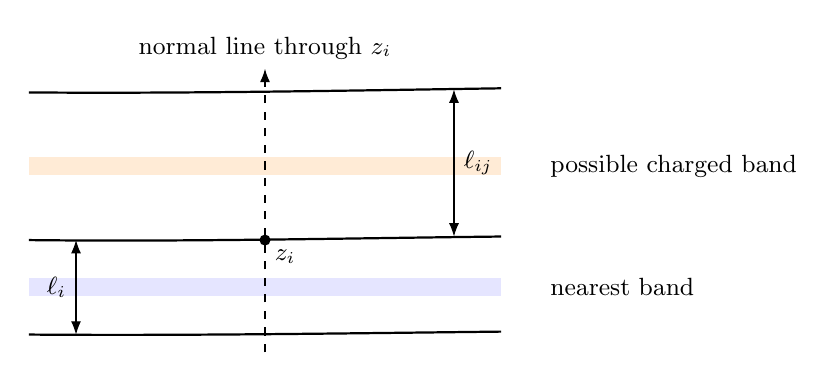
\begin{tikzpicture}[x=1cm,y=.75cm,>=Latex,font=\small]
\fill[blue!10](-3,-.95) rectangle (3,-.65);
\fill[orange!16](-3,1.1) rectangle (3,1.4);
\draw[thick](-3,-1.6).. controls(-1,-1.62)and(1,-1.58)..(3,-1.55);
\draw[thick](-3,0)..controls(-1,-.03)and(1,.03)..(3,.06);
\draw[thick](-3,2.5)..controls(-1,2.48)and(1,2.53)..(3,2.57);
\draw[dashed,->](0,-1.9)--(0,2.9) node[above]{normal line through $z_i$};
\fill(0,0)circle(2pt)node[below right]{$z_i$};
\draw[<->](-2.4,-1.6)--(-2.4,0)node[midway,left]{$\ell_i$};
\draw[<->](2.4,.06)--(2.4,2.55)node[midway,right]{$\ell_{ij}$};
\node[anchor=west]at(3.5,-.8){nearest band};
\node[anchor=west]at(3.5,1.25){possible charged band};
\end{tikzpicture}
\caption{A schematic local cross-section, not to scale. The colored strips represent fixed-width middle bands. On the part of a band assigned to $z_i$ as the larger uncut amplitude, the shorter gap $\ell_i=d(z_i)/G_1$ has vanishing normalized loss. Here $\ell_{ij}$ is the distance from $z_i$ to its first adjacent sheet on the other side. Only that side can require a positive fixed allowance. The proof uses true normal projections and does not assume globally parallel sheets.}
\label{fig:radial-interpolation}
\end{figure}

\paragraph{The finite tolerance budget.}

Since $\sqrt2/\sigma=3/4$, define
\begin{equation}\label{eq:radial-loss-number}
 C(G_1)=\frac34\sup_{u\ge0}
       e^{-\sqrt2u}(1-e^{-1.1G_1u})^2.
\end{equation}
Set $x=e^{-1.1G_1u}$ and $a_*=\sqrt2/(1.1G_1)$. Differentiation of
$x^{a_*}(1-x)^2$ shows its only interior maximum is at
$x=a_* /(a_*+2)$, while the endpoint values are zero. Hence
\begin{equation}\label{eq:radial-maximum}
 C(G_1)=\frac34
 \left(\frac{a_*}{a_*+2}\right)^{a_*}
 \left(\frac2{a_*+2}\right)^2.
\end{equation}
The defining expression is nondecreasing in $G_1$, so the largest permitted value occurs at $1.001$, and direct evaluation gives
$C(G_1)<.083272621$.

Use Young factors at most $1.001$ for the band derivative, depth cutoff, and cutoff difference. After those fixed choices, increase $R$ until the normal Jacobian, the inverse derivative $\dd s_i/\dd t$, and the exponential of the additive distance error are each at most $1.001$. After all these finite factors have been fixed, the uniform estimate following \eqref{eq:radial-one-edge} allows a normalized error of at most $.002$ on each side, including the nearest side, \emph{after multiplication by those factors}. This is legitimate because the unamplified uniform error can be made arbitrarily small.  The principal normalized switching contribution is consequently at most
\begin{equation}\label{eq:radial-finite-budget}
 \frac{.083272621}{\tanh(3\sqrt2)}
 \left(1+\frac{.001}{4}\right)^2
 \frac{32}{31.999}(1.001)^6+.004
 <.087853<.100.
\end{equation}
Every factor is finite: the band width was fixed at $3$, and all analytic tolerances were fixed before $R$ increased. In particular the proof does not use an infinite-width switch and silently discard its tails.

Choose the depth constant $M$ large enough for its negligible cost before the final increase of $R$. Then \eqref{eq:radial-test-mass} is at least
$.998\sigma\mathcal L$, and the sheet-gradient costs in
\eqref{eq:radial-tangent-cost}, including the fixed Young factor for the depth cutoff, are at most
$1.005\sigma\int|\nabla_\Sigma\psi|^2$.
The other Young factors multiply only the switch term or a tangential band term tending to zero. The rough collar and outer cutoff errors have already been shown negligible. Substitution into \eqref{eq:q-stability} and division by $\sigma$ give
\[
 (.998-.100)\mathcal L
 \le1.005\int_\Sigma|\nabla_\Sigma\psi|^2\dd S
       +o_R(\mathcal A)+o_{B\to\infty;R}(1).
\]
As $.998-.100>.895$, this proves \eqref{eq:R7}. All estimates were made at finite $B$ with coefficients uniform in $B$; the outer limit therefore precedes the limit $R\to\infty$ exactly as required by the radial argument.
\end{proof}

\subsection{The coefficient comparison and the contradiction}

The reach and stability inequalities now concern the same sheet
amplitude. Removing the derivative of its radial factor exposes the
coefficients directly; their strict differences will leave a positive
multiple of $\mathcal F T_r/\rho^2$.

The cross term against $h$ can be removed exactly:
\[
 \int_\Sigma|\nabla(hm_c\sqrt{W_*})|^2
 =\int_\Sigma\phi|\nabla(m_c\sqrt{W_*})|^2
       -\int_\Sigma h\Delta h\,m_c^2W_* ,
 \qquad
 -\frac{\Delta h}{h}
 =\frac{4+8T_r-2Hz\cdot\nu}{\rho^2}.
\]
All terms have compact support in the regular surface.
The $H$ term is $o_R(1)\mathcal L$ by \eqref{eq:R1} and
\eqref{eq:radial-scale-separation}. The derivatives of $m_c$ have
negligible cost by Lemma~\ref{lem:radial-errors}; Young's inequality
costs an arbitrarily small fixed relative loss in the other
gradient term. Since
\[
 \frac{.73(1.005)}{.895}<.820,\qquad
 \nabla\log W_*=
 \lambda\nabla(c\tau-b(d))-\frac{\vartheta}{d}\nabla d,
\]
\eqref{eq:R7}, after absorbing $o_R(1)\mathcal L$, bounds
$.73\mathcal L$, up to negligible errors, by
\[
 .835\int_\Sigma\phi m_c^2W_*
 \left[
 \frac{4+8T_r}{\rho^2}
 +\frac{1.03}{4}
 \left|\lambda\nabla(c\tau-b(d))
                 -\frac{\vartheta}{d}\nabla d\right|^2
 \right]\dd S .
\]
Every comparison with \eqref{eq:R6} is strict. For the gradient
square use $|a-b|^2\le1.5|a|^2+3|b|^2$ and
\[
 .835\frac{1.03}{4}\,1.5\lambda^2
 \le .70955\lambda<.72\,\frac{\lambda}{b'}
 \quad(0<\lambda\le2.2,\ 0<b'\le1).
\]
Its other term is
$.835(1.03)3\vartheta^2/(4d^2)$, smaller than $.012/d$
uniformly on the supported set for large $R$.
Where $\lambda=0$ the first comparison is simply unnecessary.
The constant radial terms satisfy $.835\cdot4=3.34<3.44$.
For the $T_r$ term use $\mathcal F/W_*\ge1/(2.2+o_R(1))$:
\[
 24\frac{\mathcal F}{W_*}-.835\cdot8
 \ge\bigl(24-.835\cdot8(2.2+o_R(1))\bigr)
                 \frac{\mathcal F}{W_*}
 \ge5\frac{\mathcal F}{W_*}.
\]
Subtracting and discarding the other nonnegative remainders yields
\begin{equation}\label{eq:R8}
 \int_\Sigma\phi m_c^2\mathcal F\,\frac{T_r}{\rho^2}\dd S
 \le o_R(\mathcal A)+o_{B\to\infty;R}(1).
\end{equation}
Every absorption of $o_R(1)\mathcal L$ above is performed at finite
$B$, with its coefficient uniform in $B$. Thus the exhaustion does
not presume that $\mathcal L$ has a finite limit as $B\to\infty$.

It remains to find enough surface area where the weight has not
decayed. The chosen center supplies energy of order $K(R)R^m$.
We first transfer that energy to regular zero-surface area, then use
injective normal tubes to exclude a substantial portion at large reach.

\begin{lemma}[Area at small reach]\label{lem:radial-area}
For all sufficiently large $R$, the set
\[
 \{z\in\Sigma\cap B_{2R}:m_H(z)=1,\ d(z)\le L/2\}
\]
has area at least $c K(R)R^m$, with $c>0$ independent of $R$ and
of the selected center.
\end{lemma}

\begin{proof}
The energy in $B_R$ is at least $c K(R)R^m$ by the center choice.
We first transfer a fixed fraction of it to good surface area.
Let $\mathcal Z$ be a fixed-scale separated net on all of $\Sigma$.
Uniform gradient bounds give a fixed positive lower energy in a
fixed small ball at every zero, including singular zeros.
Packing, the definition of $K$, and ball coverings show that the
number of net points in $B_{R+j+2}$ is at most
\[
 C K(R)R^m(1+j/R)^{m+1}.
\]
By \eqref{eq:phase-decay} and Modica's inequality, the energy at
points of $B_R$ whose distance from $\Sigma$ is greater than $P_0$
is therefore at most
\[
 C K(R)R^m\sum_{j\ge P_0}
 (1+j/R)^{m+1}(j+2)^n e^{-c_1j}.
\]
Choose $P_0$ large and fixed so this is a small fraction of the
initial energy. Energy within the enlarged rough collar is also
a negligible fraction: its density is bounded and its volume in
$B_{2R}$ is $O(K(R)R^{m-4+2\alpha+n\beta_0})$.
Enlarge the collar by $2P_0$ without changing this estimate.
Every remaining point lies within $P_0$ of a zero $z$ in $B_{2R}$
with $m_H(z)=1$. Such bases have $D\to0$ uniformly. Their fixed
normal tubes are regular with bounded Jacobian, and cover the
points in question by nearest projection.
Their energy is at most a fixed constant times their base area
by the area formula and the bounded energy density. Thus
\[
 \cH^m(\Sigma\cap B_{2R}\cap\{m_H=1\})\ge c K(R)R^m.
\]


The large-reach part can now be removed with the jointly injective tube
estimate from Remark~\ref{rem:reach-ordinary-tube}, applied with threshold
$L/2$. More explicitly, its normal map is injective simultaneously over
all bases with $d>L/2$ and on both normal sides for $|t|<c_2L$,
where $c_2>0$ depends only on the fixed penalty. Its Jacobian has a
fixed positive lower bound. Since $L\le R$, the images of bases in
$B_{2R}$ lie in a ball of radius at most $3R$. Consequently
\[
 \cH^m(\Sigma\cap B_{2R}\cap\{d>L/2\})
 \le C R^{m+1}/L
 =C K(R)R^m/\sqrt{K(R)}=o(K(R)R^m).
\]
Subtracting this from the preceding good-area lower bound proves the
lemma.
\end{proof}

Take $B>3R$ in \eqref{eq:R8}. On the set in
Lemma~\ref{lem:radial-area}, $m_c=1$, $\rho\le\sqrt5R$ and
$T_r\ge1/5$. Since $d\le L/2$ and $f_*(c\tau)=1$,
\[
 \mathcal F(\tau,d)\ge\int_{L/2}^L t^{-\vartheta}\dd t
 =\frac{1-2^{-(1-\vartheta)}}{1-\vartheta}L^{1-\vartheta}.
\]
Also $\phi T_r/\rho^2\ge cR^{-m}$ on $B_{2R}$.
The left side of \eqref{eq:R8} is consequently at least
$cK(R)L^{1-\vartheta}=c\mathcal A$.
First let $B\to\infty$ at fixed $R$ and then let $R\to\infty$.
This contradicts \eqref{eq:R8}. The unbounded-density alternative
is impossible.

\begin{proof}[Completion of Theorem~\ref{thm:stable}]
If a solution attains either endpoint of $[-1,1]$, it is the corresponding
constant by the strong maximum principle. The remaining constant,
zero, is unstable. Indeed, for any nonzero $\chi\in C_c^1(\R^7)$,
the test $\chi_R(x)=\chi(x/R)$ gives
\[
 Q_0(\chi_R)=R^5\int|\nabla\chi|^2-R^7\int\chi^2<0
\]
for large $R$.
For a nonconstant stable solution with values in $(-1,1)$,
if $D$ vanishes anywhere, the equality case in
Section~\ref{sec:diffuse} gives a planar heteroclinic.
Otherwise $D>0$ everywhere. If its centered density is bounded,
Theorem~\ref{thm:finite} applies. If that density were unbounded,
then $K(R)\to\infty$ and Sections~\ref{sec:reach}--\ref{sec:growth},
followed by the contradiction just proved, would apply.
Thus this last case cannot occur, and Theorem~\ref{thm:finite}
gives precisely the claimed constants and planar profiles.
\end{proof}

\appendix
\section{The dimension-nine comparison}\label{sec:dimension-nine}

There are two dimension-sensitive steps in the proof.  The classification
of the end profiles used Theorem~\ref{thm:stable} in dimension seven.
The cone argument used the absence of a singular ray in ambient dimension
eight.  In dimension nine, the singular-set bound allows dimension one,
so a vertical cylinder over a singular minimizing cone in $\R^8$
is no longer excluded.  The actual construction of del Pino, Kowalczyk,
and Wei realizes precisely this possibility.

Here the numbering refers to their published paper
\citep{DPKW2011}.  Its Theorem~1, pp.~1488--1489, constructs, for
sufficiently small fixed $\alpha>0$, a bounded entire smooth solution $u_\alpha$ in
$\R^9$, strictly increasing in $x_9$, associated with the nonaffine
entire minimal graph
\[
 \Gamma_\alpha=\{(p,F_\alpha(p)):p\in\R^8\},\qquad
 F_\alpha(p)=\alpha^{-1}F(\alpha p).
\]
It satisfies
\begin{equation}
 |u_\alpha(x)|\longrightarrow1
 \quad\text{as }\dist(x,\Gamma_\alpha)\longrightarrow\infty.
 \label{eq:monotone-dpkw-clearing}
\end{equation}
The graph is a refinement of the Bombieri--De Giorgi--Giusti construction
\citep{BDG1969}.  With
$p=(\xi,\zeta)\in\R^4\times\R^4$ and
$(|\xi|,|\zeta|)=(r\cos\theta,r\sin\theta)$, Lemma~2.1
and Theorem~2 of \citet[pp.~1492--1493]{DPKW2011} give
\begin{equation}
 \begin{gathered}
 F_0(r,\theta)=r^3g_{\rm BDG}(\theta),\qquad
 g_{\rm BDG}(\theta)>0\quad(\pi/4<\theta<\pi/2),\\
 F_0\le F\le F_0+C r^{-\beta}\min\{F_0,1\}
       \quad\text{in this sector for }r>R_0,
       \qquad 0<\beta<1,\\
 F(\zeta,\xi)=-F(\xi,\zeta).
 \end{gathered}
 \label{eq:monotone-dpkw-graph}
\end{equation}
The angular notation $g_{\rm BDG}$ is unrelated to the heteroclinic
$g$.  In arXiv version 0806.3141v2 the corresponding main and graph
theorems are numbered 1.1 and 3.1, respectively.

We spell out the consequences needed for the comparison.  For a fixed
base point $p$, continuity bounds $F_\alpha$ on every bounded
neighborhood of $p$.  Hence
$\dist((p,t),\Gamma_\alpha)\to\infty$ as $|t|\to\infty$:
otherwise a graph point a bounded distance away would have a bounded
base coordinate and an unbounded height.  Bounded strict monotonicity
gives distinct vertical limits, while
\eqref{eq:monotone-dpkw-clearing} puts both limits in $\{-1,1\}$.
They are therefore $-1$ and $1$.  In particular
$-1<u_\alpha<1$ everywhere and each vertical line has a unique zero,
of height $h_\alpha(p)$.  Equation
\eqref{eq:monotone-dpkw-clearing} also implies that all these zeros
lie within a fixed distance $D_\alpha<\infty$ of $\Gamma_\alpha$.

Fix $p$ with $0<|\xi|<|\zeta|$ and fix $t\in\R$.
The angular direction stays in a compact subinterval of the positive
sector for all points $Rp+O(1)$ as $R\to\infty$.  The lower bound
in \eqref{eq:monotone-dpkw-graph}, with $\alpha$ fixed, gives
\begin{equation}
 F_\alpha(Rp+O(1))\ge c_{p,\alpha}R^3
 \quad\text{for all sufficiently large }R.
 \label{eq:monotone-dpkw-cubic}
\end{equation}
A graph point within $D_\alpha+1$ of the zero
$(Rp,h_\alpha(Rp))$ has base coordinate $Rp+O(1)$, so
\eqref{eq:monotone-dpkw-cubic} implies
$h_\alpha(Rp)/R\to+\infty$.  Thus $u_\alpha(Rp,Rt)<0$ for
large $R$.  Moreover the distance from $(Rp,Rt)$ to the graph tends
to infinity: a bounded-distance subsequence would contradict
\eqref{eq:monotone-dpkw-cubic}.  By
\eqref{eq:monotone-dpkw-clearing},
\[
 u_\alpha(Rp,Rt)\longrightarrow-1
           \quad\text{if }0<|\xi|<|\zeta|.
\]
The oddness of $F$ and the same argument give limit $+1$ in the
opposite sector $0<|\zeta|<|\xi|$.  The excluded equality set and
coordinate axes have Lebesgue measure zero.  Bounded convergence now
shows local $L^1$ convergence of the rescaled solutions to the two-phase
function with interface
\begin{equation}
 \mathcal C_9=
      \{(\xi,\zeta):|\xi|=|\zeta|\}\times\R.
 \label{eq:monotone-dpkw-cylinder}
\end{equation}
This cone has the entire vertical axis as its singular set and is
invariant under vertical translations.  Its directional normal
component is zero on its regular part.  Thus it falls into exactly the
case that was ruled out by the singular-set bound in
Lemma~\ref{lem:monotone-flat-cone} in dimension eight.

The same solutions are minimizers by
Lemma~\ref{lem:monotone-minimizer}, applied to their constant end
profiles, and consequently have the corresponding $O(R^8)$ energy
growth.  Thus neither the derived minimizing property nor this energy
bound conflicts with the construction.  Their nonplanar phase limit
also precludes one-dimensionality.  The construction extends constantly
in additional coordinates to every $N>9$, as explained in
\citet[p.~1490]{DPKW2011}: the added second derivatives vanish, and
strict monotonicity in $x_9$ is preserved.  It supplies no
eight-dimensional example.

\bibliographystyle{plainnat}
\bibliography{refs}
\end{document}
